\documentclass[english]{amu_these}
\begin{document}

	\selectlanguage{english}										
	
	\chead{}
\pdfbookmark[0]{Page de titre}{titre}
\thispagestyle{empty}
\newgeometry{margin=2em}
% \newgeometry{left=3em,right=2em,top=2em,bottom=2em} %% marge pour la reliure en cas d'exemplaire imprimé

\vspace{1em}

\begin{center}
	\begin{minipage}[c]{.5\linewidth}
		\raggedright\includegraphics[height=7em]{logo_amu}
	\end{minipage}\hfill
	\begin{minipage}[c]{.5\linewidth}
		%\raggedleft\includegraphics[height=7em]{example-image-b} %% logo établissement en cotutelle, le cas échéant
	\end{minipage}\hfill
\end{center}

%\vspace{.4em}

\begin{center}
	\begin{minipage}[c]{.77\linewidth}
		\textcolor{yellowamu}{\noindent\rule{\textwidth}{4pt}}
	\end{minipage}\hfill
	\begin{minipage}[c]{.23\linewidth}
		\raggedleft\textsf{NNT : 2024AIXM0001}
		% renseigner votre numéro national de thèse (NNT)
	\end{minipage}\hfill
\end{center}

%\vspace{1em}

\doublespacing
\begin{flushleft}
    \textsf{\HUGE\textcolor{blueamu}{THÈSE DE DOCTORAT}}\\
	\textsf{\Large Soutenue à AMU ― Aix-Marseille Université}\\
	%\textsf{\Large dans le cadre d'une cotutelle avec }\\ %% établissement en cotutelle, le cas échéant
	\textsf{\Large le ... décembre 2024 par}\\
\end{flushleft}
\vspace{1.5em}
\begin{center}
	\textsf{\textbf{\Huge Raffael DÜLL}}\\
    \vspace{1em}
	\textsf{\LARGE SIMULATING EDGE PLASMA TURBULENCE FOR ITER:}\\ 
	\textsf{\Large Improving the numerical resolution of a very anisotropic, poorly conditioned diffusion problem}\\
\end{center}
\singlespacing

%\vspace{2em}

\begin{center}
	\begin{minipage}[t]{.37\linewidth}
    	    \vspace{.5em}
        	\textsf{\textbf{Discipline}}
        	
        	\textsf{Sciences pour l'Ingénieur}
        	
    	    \vspace{1em}
        	\textsf{\textbf{Spécialité}}
        	
        	\textsf{Fusion magnétique}
        	
    	    \vspace{2em}
        	\textsf{\textbf{École doctorale}}
        	
        	\textsf{ED 353 SCIENCES POUR L'INGÉNIEUR: MECANIQUE, PHYSIQUE, MICRO ET NANOELECTRONIQUE}
        	
    	    \vspace{1em}
        	\textsf{\textbf{Partenaires de recherche}}
        	
        	\textsf{Laboratoire de Mécanique, Modélisation \& Procédés Propres (M2P2), AMU}
    	    \vspace{0.4em}			        	
        	\textsf{Institut de Recherche sur la Fusion par Confinement Magnétique (IRFM), CEA Cadarache}

	\end{minipage}\hfill
	\begin{minipage}[t]{.02\linewidth}
		\centering
	    \rule[-280pt]{1pt}{280pt}
	\end{minipage}\hfill
	\begin{minipage}[t]{.6\linewidth}
	    \vspace{.5em}
    	\textsf{\textbf{Composition du jury}}

	    \vspace{1em}
    	\textsf{
        \begin{tabular}{p{14em} p{10em}}
        	Benjamin DUDSON & Rapporteur \\
        	{\small Lawrence Livermore National} \\ {\small Laboratory} \\
        	\\
        	Boniface NKONGA & Rapporteur \\
        	{\small Université Nice Sophia Antipolis} \\
            \\
            Daniela GRASSO & Examinatrice \\
        	{\small Politecnico di Torino} \\
            \\
        	Paolo RICCI & Président du jury \\
        	{\small Swiss Plasma Center, EPFL} \\
            \\
        	Eric SERRE & Directeur de thèse \\
        	{\small Aix-Marseille Université, CNRS} \\
            \\
			Hugo BUFFERAND & Encadrant de thèse \\
			{\small CEA/IRFM} \\
           \\
        	Xavier GARBET & Membre invité \\
        	{\small Nanyang Technological} \\ {\small University} \\
        \end{tabular}
    }
	\end{minipage}\hfill
\end{center}       

\vspace{2em}

\begin{center}
	%% logos partenaires
	\begin{minipage}[c]{.25\linewidth} 
		\centering\includegraphics[height=5em]{logo/logo_IRFM.jpg}
	\end{minipage}\hspace{0.05\linewidth} 
	\begin{minipage}[c]{.25\linewidth} 
		\centering\includegraphics[height=5em]{logo/logo_M2P2.png}
	\end{minipage}\hspace{0.05\linewidth}
	\begin{minipage}[c]{.35\linewidth} 
		\centering\includegraphics[height=5em]{logo/logo_eurofusion.png}
	\end{minipage}
\end{center}

\restoregeometry
				%% page de titre
										
	\input{tex_open/affidavit}				%% affidavit et licence

	\newpage
\addchap{List of publications and/or patents and conference participation}
\label{chap:publications}
\addsec*{(1) List of publications and/or patents produced as part of the thesis project:}
\begin{enumerate}
\item \textbf{Düll, R.}, Bufferand, H., Serre, E., Ciraolo, G., Quadri, V., Rivals, N. and Tamain, P., 2024. Introducing electromagnetic effects in Soledge3X. \textit{Contributions to Plasma Physics}, p.e202300147.
\item \textbf{Düll, R.}, Ciraolo, G. Bufferand, H., Serre, E.,, Quadri, V., Rivals, N., Tamain, P., Sureshkumar, S. and Varadarajan, N. Implementation of a non-axisymmetric magnetic configuration in SOLEDGE3X to simulate 3D toroidal magnetic ripple effects: Application to WEST. \textit{Nuclear Materials and Energy} [under review]
\item \textbf{Düll, R.}, Bufferand, H., Serre, E., Ciraolo, G., Quadri, V., Rivals, N., Schwander, F. and Tamain, P., An electromagnetic model in SOLEDGE3X for edge plasma turbulence simulations in tokamak. \textit{Journal of Computational Physics} [to be submitted]
\item Quadri, V., Tamain, P., Marandet, Y., Bufferand, H., Rivals, N., Ciraolo, G., Falchetto, G., \textbf{Düll, R.} and Yang, H., 2024. Self‐organization of plasma edge turbulence in interaction with recycling neutrals. \textit{Contributions to Plasma Physics}, p.e202300146.
\item  Quadri, V., Tamain, P., Marandet, Y., Bufferand, H., Rivals, N., Ciraolo, G., Falchetto, G.L., \textbf{Düll, R.}, Sureshkumar, S., Varadarajan, N. and Yang, H., 2024. Edge plasma turbulence simulations in detached regimes with the SOLEDGE3X code. \textit{Nuclear Materials and Energy}, p.101756.
\item De Gianni, L., Ciraolo, G., Giruzzi, G., Falchetto, G., Rivals, N., Balbinot, L., Varadarajan, N., Sureshkumar, S., Artaud, J.F., Bufferand, H. and \textbf{Düll, R.}, Core and edge modeling of JT-60SA H-mode highly radiative scenarios using SOLEDGE3X-EIRENE and METIS codes. \textit{Frontiers in Physics}, 12, p.1422286.
\end{enumerate}

\newpage

\addsec*{(2) Participation in conferences and summer schools during the thesis period:}
\begin{enumerate}
\item Summer School PlasmaSurf by Instituto de Plasmas e Fus\~{a}o Nuclear. July 2022, Lisbon, Portugal
\item Conference EPS - 49th European Conference on Plasma Physics, European Physical Society. July 2023, Bordeaux, France. Poster presenation: \textit{"A new electromagnetic model in SOLEDGE3X"}
\item Conference PET19 - 19th International Workshop on Plasma Edge Theory in Fusion Devices. September 2023, Hefei, China. Contributed talk: \textit{"Introducing electromagnetic effects in Soledge3X"}
\item Conference PSI-26 - 26th International Conference on Plasma Surface Interaction in Controlled Fusion Devices. May 2024, Marseille, France. Poster presentation: \textit{"Electromagnetic effects on turbulent structures in edge plasmas with SOLEDGE3X"}
\item EUROfusion - TSVV3 Annual Workshop. May 2024, Leuven, Belgium [remote participation]. Presentation: \textit{"Simulating electromagnetic effects in SOLEDGE3X"}
\item Conference ECCOMAS - 9th European Congress on Computational Methods in Applied Sciences and Engineering. June 2024, Lisbon, Portugal. Participation at the mini-symposium: Magnetohydrodinamic Numerical Modeling of Magnetised Plasmas. I with the oral presentation: \textit{"An electromagnetic model for SOLEDGE3X"}
\item EUROfusion - TSVV1 Progress Workshop. September 2024, Garching, Germany. Presentation: \textit{"A new electromagnetic model for turbulent simulations in SOLEDGE3X"}
\end{enumerate}			%% liste de publications et participation aux conférences

	\addchap{Résumé et mots clés}
\label{chap:resume}

\selectlanguage{french}

\lipsum[1]\index{Lorem ipsum}

\vspace{0.5cm}
Mots clés: géométrie algorithmique, complexe planaire et rectangulaire, géodésique, courbure globale non-positive
\selectlanguage{english}										

					%% résumé

	\addchap{Abstract and keywords}
\label{chap:abstract}

In the tokamak edge, steep gradients and magnetic curvature generate large-scale turbulent structures that transport plasma particles from the hot core, where fusion occurs at around 10 keV, to the much colder Scrape-Off-Layer (SOL), where magnetic field lines intersect the physical wall. Turbulence reduces plasma confinement and defines the region where strong heat fluxes impact the divertor. The drift-reduced fluid code SOLEDGE3X, developed by CEA/IRFM in collaboration with Aix-Marseille University, has proven effective in simulating electrostatic resistive drift-wave turbulence in realistic tokamak geometries. However, both experimental and numerical results have shown that electromagnetic effects significantly impact drift-wave dynamics, and thus, edge plasma turbulence. 

This thesis introduces a new electromagnetic model in SOLEDGE3X for the vorticity equation, incorporating magnetic induction, electromagnetic flutter, and electron inertia. Magnetic induction accounts for the time variation of the parallel magnetic vector potential $A_\parallel$ in the definition of the parallel electric field, and $A_\parallel$ is related to the parallel current density $j_\parallel$ via Ampère's law. Fluctuations in the magnetic field, termed flutter, are added at first order and are assumed to be small compared to the equilibrium field. Electron inertia, represented by a finite electron mass in Ohm's law, is necessary to constrain shear Alfvén wave speeds to physical values. The new fields $A_\parallel$ and $j_\parallel$ are integrated into the flux-surface-aligned FVM framework on a poloidally and toroidally staggered grid. Flutter affects the parallel transport equations and gradients in Ohm's law, and its implementation required special care to account for the new radial component of the parallel direction $\textbf{b}$. To handle timesteps larger than Alfvénic, electron thermal, or electron-ion collision times, the corresponding inductive, inertial, and resistive effects are solved implicitly in a coupled 3D system for the potentials $\Phi$ and $A_\parallel$. The model was verified with manufactured solutions and validated on a linear slab case, which demonstrated the expected transition from Alfvén to thermal electron waves as the perpendicular wavenumber increased. 

Flutter contributes minimally to cross-field transport but affects the non-adiabatic potential response to density fluctuations in Ohm's law. Simulations in slab, circular (limited), and X-point (diverted) geometries consistently show that electron inertia and magnetic induction destabilize drift-wave turbulence, while flutter stabilizes it in both the linear and nonlinear phases. On open field lines, magnetic induction reduces the sensitivity of turbulent structures to sheath effects, promoting further turbulence spreading in the SOL. Numerically, electron inertia significantly improves the condition number of the vorticity system, especially in hot plasmas with low resistivity, providing a factor-four speedup even in electrostatic scenarios. However, adding flutter degrades code performance, as it requires solving implicit 3D systems for viscosity and heat diffusion problems that were previously treated as uncoupled 2D systems on each flux surface. As an extension to this work, perturbations to the magnetic equilibrium were externally imposed in a transport mode simulation to study heat deposition in a non-axisymmetric magnetic configuration with ripple on WEST.

\vspace{0.5cm}
Keywords: tokamak, edge plasma, turbulent simulations, electromagnetism, SOLEDGE3X
				%% abstract

	\addchap{Acknowledgments}

I want to thank IRFM and Aix-Marseille University for allowing me to pursue and complete this PhD thesis over the past three years. It has been a journey with ups and downs, stretching across moments of fervent excitement and nerve-wracking struggles.

I am very grateful to my academic supervisor, Eric Serre, for his guidance and support throughout this process. His encouragement, foresight, and feedback have been invaluable for this work. He knew what to prioritize and focus on at any moment, and as such I could stay on course with a clear goal before me.

Equally, my advisor, Hugo Bufferand, was my daily support throughout this endeavour. He accompanied me from my first steps in the world of plasma physics to deep and precise questioning. I truly enjoyed our many conversations about the requirements and possibilities of the model and its best implementation. Your clarity in explaining complex concepts and availability to address my endless questions have been priceless. This thesis owes much to your guidance and support.

I want to thank Patrick Tamain for his help with the code framework and all the caveats I had to be aware of. I am equally grateful for his perspective and feedback on the physical model I was working on. I never forget our endless but fruitful Monday morning developer discussions. Without your involvement, my developments would undoubtedly have remained buried in a forgotten branch of the repository and unseen by any potential user. 

I am also grateful for the enriching discussions on plasma theory with various institute colleagues. First, I would like to thank Frédéric Schwander, whose insights into fluid models helped clarify many aspects of my work. Yanick Sarazin, I appreciated our conversations about the theory of edge plasma turbulence dynamics. Finally, Eric Nardon, you helped to bridge the gap between the new electromagnetic fluid approach and state-of-the-art MHD models.

I want to thank the members of my PhD jury for taking the time to read my manuscript, traveling to Cadarache for those who could, and asking thoughtful questions during the defense. 

During my time at CEA, I had the chance to meet some fantastic people who made this journey very enjoyable. We almost lived like a small family in the unpretentious building 513, safeguarded by our ever-watchful, hairy boar guardians. Virginia, Yann, Olivier, Mattia, Jai, Kévin, Robin, Nicolas, Hao, Emily, Srikanth, Ludovica, Roméo, Naren - we all know what it means to lose the mind on a single question for several years. And yet, we still found our moments of fun, whether during the coffee breaks or over beers in the uncountable Plasmapéros. For my two successive office mates, Robin and Srikanth, I apologize for driving you crazy with my constant random remarks; Virginia, thanks for being the best travel mate on the epic journey to China; Ludovica, you taught me more Italian than anything I learned during the PhD. I even talked to people in the neighbouring buildings! Quentin, with whom I ended up cycling along the Mediterranean coast; Théo, we still need to beat skiing records; Mathieu, soon will come the day we open a restaurant. A special note to Michele, who just arrived in this parallel universe: best of luck—I’m sure you’ll do great! I also want to acknowledge the people at the M2P2 lab. I have great memories of the conference trip to Portugal with Eduardo, Hippolyte, and Tom. Although I didn’t visit the lab as often as I’d have liked, I’m looking forward to reconnecting more during my postdoc.

Moving to Marseille for my PhD turned out to be one of the best decisions I ever made. I quickly grew to love the city, its vibrant atmosphere, and the wonderful people I met there. I’ll always have fond memories of my time there.

Finally, a big thank you to my family for always being there for me. Your support has meant a lot.

And last but not least, thanks to you, the reader, for making it this far. The fact that you took the time to read this thesis really means a lot to me, and I know you will read past this Acknowledgements section. Thank you!				%% remerciements

    \microtypesetup{protrusion=false}	%% désactive la protrusion (TOC LOFT GLS)
	\tableofcontents					%% TOC
	\listoffigures						%% LOF
	\listoftables						%% LOT
	\printglossary[						%% acronymes
		type=\acronymtype,
		title={List of acronymes},
		toctitle={List of acronymes}
		]
	\printglossary[						%% glossaire
		title={Glossary},
		toctitle={Glossary}
		]
	\printglossary[						%% nomenclature
		type=notation,
		title={Naming convention},
		toctitle={Naming convention}
		]
    \microtypesetup{protrusion=true}	%% rétabli la protrusion

	\ohead{\leftmark\Ifstr{\rightmark}{\leftmark}{}{ -- \rightmark}}	%% place le chapître et la partie en en-tête
	
	\clearpage
	
	\chapter{Introduction}
\label{chap:Intro}
The sun is the primary source of energy for Earth, essential for photosynthesis in plants, which forms the basis of most food chains, and for driving the weather and climate systems that shape our environment. Its consistent radiation supports all life forms, regulates global temperatures, and influences fundamental ecological and biological processes that are vital for the Earth's diverse ecosystems. From the very outset of human life, the sun has been a subject of profound admiration, occupying a central role in various religious beliefs and was often synonym of an incomparably vast and potent source of energy. It was not until the beginning of the twentieth century that progress in particle physics allowed to unravel the secret of solar energy: nuclear fusion. It is the physical process where two light atoms merge to form a heavier atom, releasing significant energy as a result of mass-to-energy conversion. The strong nuclear force is fundamental to confine the positivily charged protons with neutrons in an atomic nucleus. Every element is characterized by its total binding energy, that corresponds to the energy needed to break an atom into its constituting protons and neutrons. A higher total binding energy means that the element is more stable. The maximum binding energy is observed for iron ($^{56}Fe$), it means that (roughly) all lighter elements can produce energy by fusion and heavier by fission, as it is done in conventional nuclear power plants.  \newline 

The dream of achieving nuclear fusion in a laboratory to produce energy emerged shortly thereafter. In today's climate crisis, nuclear fusion is even more appealing because it does not emit carbon emissions, does not present the risk of a catastrophic meltdown and its fuel, hydrogen, is readily available. Since replicating the sun's core conditions on Earth, particularly the immense pressure, is not feasible, alternative approaches were searched. A look at Fig. \ref{fig:Intro_fusionCrossSections} with the reaction cross-section of various pairs of light atoms shows that deuterium-tritium (D-T) fusion has the highest likelihood at the most accessible temperature. These two hydrogen isotopes are hence the most favorable candidates for fusion; deuterium is naturally abundant, but tritium, which is radioactive and has a relatively short half-life, must be artificially produced. The reaction reads: \newline

\begin{equation}
	^2_1D + ^3_1T \Rightarrow ^4_2He [3.5MeV] \quad + ^1_0n [14.1 MeV]
\end{equation}

\begin{figure}[H]
	\centering
	\includegraphics[width=0.62\textwidth]{schemes/fusion-xsecs2.png}
	\caption{Fusion reaction cross-sections for the most promising pairs of light elements over center-of-mass energy.}
	\label{fig:Intro_fusionCrossSections}
\end{figure}

In the fusion reaction between deuterium and tritium, one alpha-particle (or Helium-4 nucleus) and one neutron are produced. 80\% of the released energy is carried by the neutron. At such elevated temperatures, the electromagnetic force is insufficient to maintain the cohesion of electrons and their atomic nuclei, resulting in the formation of a state of matter known as plasma. Plasma is an ionized gas composed of positively charged nuclei and negatively charged electrons, which interact electromagnetically. \newline

Lawson's criterion \cite{Lawson1957} estimates the necessary plasma conditions to reach the break-even point, where fusion power exceeds heating and conduction losses. For D-T fusion, the triple product of density $n$, temperature $T$, and energy confinement time $\tau_E$ must exceed:

\begin{equation}
	\label{eq:LawsonCriterionDT}
	nT\tau_E > 10^{-21} \, \text{keV} \cdot \text{m}^{-3} \cdot \text{s}
\end{equation}

From a practical point of view, an important metric is the fusion gain $Q$, which measures the ratio of power produced in the nuclear fusion reaction to the required heating power to maintain plasma conditions. One major milestone is the break-even point, when the fusion reaction produces enough power to maintain a steady state at $Q=1$. However, the plasma can only capture a fraction of the produced fusion energy, as most fast neutrons rapidly escape the plasma, with, as seen before, 80\% of the energy. Therefore, external heating is still required until $Q>5$. Past this point, fusion produces more heat than the total required heating power and sustains itself in a state known as ignition ($Q=\infty$). Commercial operation of fusion power plants requires reliable access to ignition, which still requires decades of research. \\

The reaction cross-section determines an optimal temperature of approximately 15-40 keV (~150 million °C) for D-T fusion reactions, leading fusion reactor designs to maximize either of the two remaining parameters: density or confinement time. There is a large variety of approaches to artificial fusion, but today, two concepts show the most promise. Inertial Confinement Fusion (ICF) seeks to compress dense fuel pellets for an extremely brief duration using high-powered lasers. Conversely, Magnetic Confinement Fusion (MCF) utilizes strong magnetic fields to sustain stable plasmas at relatively low densities. Within MCF, there are two primary designs: tokamaks, which use a toroidal chamber with an axisymmetric magnetic field, and stellarators, which use a twisted magnetic configuration to improve plasma confinement.\\

Figure \ref{fig:Intro_fusionTripleProduct} depicts the current status of fusion experiments with respect to Lawson's criterion. On December 5, 2022, the National Ignition Facility (NIF) reached the break-even point for the first time, achieving a 3.1 MJ fusion yield with 2 MJ of injected laser power \cite{abu2024achievement}. Large MCF devices, such as DIII-D, TFTR, JET, and JT60-SA, are already very close to the break-even point. Next-generation devices, including ITER and SPARC, which are under construction, are expected to achieve $Q>1$. \\

\begin{figure}[H]
	\centering
	\includegraphics[width=0.7\textwidth]{schemes/Fusion_Triples_2021.png}
	\caption{Relation of the fusion trapping $n\tau_E$ to the temperature in current and future devices. For MCF The break-even point (Q=1) corresponds to the green area and ignition (Q=$\infty$) is brown. Ignition for ICF is reached at the solid black line. Taken from \cite{wurzel2022progress}}
	\label{fig:Intro_fusionTripleProduct}
\end{figure}

In this work, we focus on the most promising candidate for MCF, the tokamak. The three Soviet physicists Lavrent'ev, Sakharov, and Tamm had the idea in the early 1950s \cite{azizov2012tokamaks} to confine the plasma in a strong toroidal magnetic field. Additional coils create a poloidal field to suppress instabilities, such that plasma particles are trapped on helical trajectories. The first experiment was conducted in 1954 at the LIPAN institute in Moscow, the predecessor of the Kurchatov institute. The term "tokamak" or "\cyrillic{токамак}" was coined in 1957 by Golovin, and is a Russian acronym of "\cyrillic{тороидальная камера с магнитными катушками}", which translates to "toroidal chamber with magnetic coils," where the "G" from "mag" was transformed to "K" for better sonority \cite{shafranov1999trends}. \\

Since then, tokamaks gained popularity in the USSR and abroad. The design was improved with each generation of new devices to operate at ever higher power. In the 1960s, the first devices surpassed the Bohm limit. Technological progress in plasma heating and superconducting coils led to second-generation tokamaks, such as TFTR and JET, which could operate at much higher temperatures and magnetic field strengths. Another breakthrough was the refined shaping of the magnetic equilibrium with the introduction of divertors to carefully direct particle fluxes, which ultimately culminated in the discovery of the high-confinement (H) mode, allowing for much higher core temperatures. The largest fusion experiment, ITER, is currently under construction in southern France by an international collaboration of seven member parties. At full operation, it is expected to achieve ignition, a state where the fusion reaction emits sufficient radiation to maintain plasma conditions. Its scientific goals include maintaining burning plasma for an extended period of time and demonstrating safe operation in the nuclear phase. It will also serve as a test facility for tritium breeding blankets, a much-needed technology to produce tritium in situ. Currently, tritium is only obtained in pressurized water reactors, and the worldwide annual production of about 500 g is far insufficient to meet the required 55.8 kg per GW installed in a fusion power plant \cite{abdou2020physics}. \\

Much of the research in fusion energy is dedicated to understanding fundamental physical processes in the plasma and projecting behavior in future machines. Due to the harsh conditions inside the tokamak vessel, diagnostics can only measure indirect properties of the core plasma and are limited in spatial resolution. Simulations offer a powerful tool to construct a digital twin of the device, where physical processes can be correlated and better understood. One particular region of interest is the transition from the hot core region with closed magnetic field lines to the edge and the scrape-off layer, where particles traveling along the magnetic field collide with the physical wall in the divertor region. Strong temperature gradients lead to large turbulent structures, driven by resistive drift waves. It is crucial to understand the dynamics and interactions with impurities or neutrals, as fluxes crossing the separatrix largely define the quality of plasma confinement. From a material design perspective, edge plasma simulations are essential to characterize the particle and heat fluxes on the physical wall. \\

One  major simulation framework that serves this very purpose is the SOLEDGE3X code, originally developed at CEA Cadarache, and extended in the scope of this thesis. Currently, turbulent simulations are limited to L-modes and small machines due to numerical issues and a limited model for larger machines. A significant limitation arises from the anisotropy between the parallel (resistive) and perpendicular (from the time evolution of the vorticity) Laplacians acting on the electric potential. This becomes problematic when the resistivity is very small. Even in the electrostatic collisional regime found in the plasma edge, electron inertia and electromagnetic effects play a substantial role, especially as electron inertia replaces resistivity as it approaches zero. \\

The current implementation of SOLEDGE3X is primarily limited to simulating L-mode plasmas and smaller tokamaks due to various numerical challenges and the limited applicability of its models to larger machines. A significant limitation arises from the anisotropy between the parallel (resistive) and perpendicular (vorticity-driven) Laplacians acting on the electric potential. In the existing electromagnetic model, the vorticity equation is solved implicitly, and as the resistivity approaches zero, the condition number of the matrix deteriorates considerably. Even in the electrostatic, collisional regime typically found in edge plasma, electron inertia and electromagnetic effects play a crucial role, and notably, the finite electron mass in Ohm's law acts as a lower bound for the resistivity. \\

As the plasma approaches the L-H transition, electromagnetic effects become increasingly important. The H-mode is characterized by a suppression of cross-field transport due to "ExB" drifts, which are partially replaced by electromagnetic transport. Significant magnetic reconnection processes lead to important transport of plasma particles from the hot core to the cold edge, with radial fluxes still below "ExB" advection, but non-negligible in understanding the overall plasma behavior. \\

This thesis is dedicated to the implementation of an electromagnetic model within SOLEDGE3X, which includes magnetic induction in the parallel electric field, perturbations of the magnetic equilibrium (flutter), and a finite electron mass in Ohm's law. This development pursues several goals: first, it improves the accuracy of the physical model; second, it enhances numerical robustness by mitigating the poor matrix conditioning associated with low resistivity; and third, it establishes a foundation for self-consistent turbulent simulations that are relevant to larger machines and higher-power scenarios. \\

!!!!!!! PRESENT CHAPTERS OF THE THESIS !!!!!!!!!!


	
	\part[Fundamental Concepts of Fluid Models for Magnetized Plasmas]{Fundamental Concepts of Fluid Models for Magnetized Plasmas}
	\label{part:FundamentalsPlasmaSimulations}
	\chapter{Tokamak Concept}
\label{chap:TokamakConcept}

\vfill
\begin{chaptersummarybox}
	With a given initial velocity, charged particles travel along magnetic field lines on a circular trajectory with the Larmor radius $\rho_L$ and cyclotron frequency $\omega_B$. 
	\begin{align*}
		\rho_L   &= \frac{m\norm{\mathbf{v}_{\perp,0}}}{qB} &
		\omega_B &= \frac{qB}{m}
	\end{align*}	
	Any force perpendicular to the magnetic field causes particles to drift with the velocity $\mathbf{v}_d = \frac{\mathbf{B}\cross\mathbf{F}_\perp}{qB^2}$. To control particle motion, tokamaks employ toroidal and poloidal magnetic fields $B_{\varphi}$ and $B_{p}$ to shape a helical configuration around a torus. To compensate for plasma currents, the magnetohydrodynamic equilibrium causes the so-called Grad-Shafranov shift, which pushes the poloidal field outward. A low ratio between thermodynamic to magnetic pressure, $\beta = \frac{neT}{B^2/2\mu_0}$, is important to avoid plasma instabilities. \\
	At scales beyond the Debye length $\lambda_D = \sqrt{\frac{\varepsilon_0T_e}{n_ee^2}}$, the plasma organizes itself in a state of quasi-neutrality. Collisions between particles cause momentum, energy and charge exchanges, leading to viscosity, heat diffusion and resistivity according to the Spitzer-Härm model:
	\begin{align*}
		\nu_{SH}    &\propto \frac{T_e^{5/2}}{Z^4 \ln \Lambda} &
		\kappa_{SH} &\propto \frac{T_e^{5/2}}{Z \ln \Lambda}   &
		\eta_{SH}   &\propto\frac{Z \ln \Lambda}{T_e^{3/2}}
	\end{align*}
	At the sheath, where magnetic field lines intersect the tokamak wall, a net negative charge develops that attracts ions at high speeds. In divertors, the heat exhaust is concentrated on two thin target lines, and the width $\lambda_q$ is critical for reactor designs.
\end{chaptersummarybox}
\vfill

\newpage

Fusion reactions require extreme temperatures at about 15keV to happen. At such high temperatures, any matter transforms into an ionized state, called plasma, where electrons are dissociated from their atomic core. Charged particles are particularly responsive to magnetic fields, a property that will be used by tokamaks to confine the hot plasma and protect the physical walls of the device. 

A deuterium plasma is an ionized gas comprising positively charged ions ($D^+$) and negatively charged electrons ($e^-$). Initially, both species exhibit independent dynamics. Despite having exactly opposite charges, ions are significantly heavier than electrons, with a mass ratio of $m_i/m_e \approx 3.7\cdot 10^3$. Both ions and electrons can be described by their respective momenta and temperatures. In Sec. \ref{sec:intro_particlesInPlasma}, we first describe their independent behavior in a magnetized environment, then how species interact in Sec. \ref{sec:intro_particlesInteration} and we finish with Sec. \ref{sec:intro_SOL} about the importance of the Scrape-Off-Layer.


\section{Particles in a magnetized plasma}
\label{sec:intro_particlesInPlasma}

This first section describes the fundamental working principle of plasma confined in a tokamaks. Before all, we must understand how charged particles behave when exposed to strong magnetic fields (in Sec. \ref{ssec:intro_magneticConfinement}) and how they experience drifts in perpendicular direction (in Sec. \ref{ssec:intro_plasmaDrifts}). This knowledge allows us to design a magnetic "cage", in which particles are trapped, or confined (in Sec. \ref{ssec:intro_tokamakConfiguration}). The governing equations of this magnetic configuration are given in Sec. \ref{sec:intro_GradShafranov} and Sec. \ref{ssec:intro_limitedDivertedConfig} introduces and compares limited and diverted configurations.

\subsection{Gyromotion of a single particle}
\label{ssec:intro_magneticConfinement}
To understand how charged plasma particles can be confined on a magnetic field line, we consider the simplest example of a single particle with charge \( q \) in a homogeneous, unidirectional magnetic field \(\textbf{B}\) with directional unit vector \(\textbf{b}\). The amplitude of the magnetic field is then $B$ such that $\mathbf{B} = B\mathbf{b}$. Solely the magnetic component of Lorentz's force acts on a particle with mass \( m \) and charge \( q \), leading to the following equation for its velocity \(\textbf{v}\):

\begin{equation}
	\label{eq:gyromotion_LorentzForce}
	m\dv{\textbf{v}}{t} = q\textbf{v}\cross\textbf{B}
\end{equation}

To solve this differential equation, it is convenient to decompose the velocity vector into a parallel component \( v_\parallel = \textbf{v}\cdot\textbf{b} \) and a perpendicular component \( \textbf{v}_\perp = \textbf{v} - v_\parallel \textbf{b} \). For a given initial velocity \(\mathbf{v}_0\), the general solution of this system is:

\begin{equation}
	\mathbf{v}(t) = v_{\parallel,0}\mathbf{b} + \mathbf{v}_{\perp,0}\cos(\omega_B t) + \mathbf{b} \times \mathbf{v}_{\perp,0} \sin(\omega_B t)
\end{equation}

with \(\omega_B = \frac{qB}{m}\) being the cyclotron frequency. This implies that a charged particle circles around a magnetic field line while following it with its initial velocity. The opposite charges of ions and electrons result in them circling in different directions. The trajectory is qualitatively shown in Fig. \ref{fig:TokamakBasics_gyromotion}. The radius of this gyromotion is called the Larmor radius \(\rho_L\):

\begin{equation}
	\rho_L = \frac{m\norm{\mathbf{v}_{\perp,0}}}{qB}
\end{equation}

Because of the high mass ratio, ions have a much larger Larmor radius than electrons. This gyromotion is the fundamental mechanism behind magnetic confinement. \newline 


\begin{figure}[H]
	\centering
	\includegraphics[width=0.62\textwidth]{schemes/gyromotion.png}
	\caption{Trajectory of a positively and a negatively charged particle along a homogeneous magnetic field line.}
	\label{fig:TokamakBasics_gyromotion}
\end{figure}


For a non-homogeneous field, Eq. \ref{eq:gyromotion_LorentzForce} does not necessarily have a straightforward solution. To assume gyromotion as the fundamental dynamic for particles, the magnetic field must remain relatively constant along the helical path traced by the field lines. This requirement imposes a criterion on the Larmor radius, known as adiabatic theory:
\begin{equation}
	\label{eq:intro_adiabaticCondition}
	\rho_L \ll \frac{B}{\norm{\grad B}}
\end{equation}


\subsection{Plasma drifts}
\label{ssec:intro_plasmaDrifts}

Plasma drifts refer to the movement of charged particles under the influence of electric and magnetic fields. These drifts do not account for the primary motion along the guiding center, as described in Section \ref{ssec:intro_magneticConfinement}. To study drift velocities, it is convenient to decompose every vector quantity into an average parallel component and a fluctuating perpendicular component, such that $\mathbf{X} = X_\parallel\mathbf{b} + \mathbf{X_\perp}$. We then express the Lorentz force equation as:

\begin{equation}
	\label{eq:edge_LorentzEquationDecomposition}
	m\partial_t\left(v_\parallel\mathbf{b} + \mathbf{v}_\perp\right) = q\left[E_\parallel\mathbf{b} + \mathbf{E}_\perp + \left(v_\parallel\mathbf{b} + \mathbf{v}_\perp\right) \times \mathbf{B}\right]
\end{equation}

Focusing on the particle's acceleration in the perpendicular direction, we derive the equation of motion:

\begin{equation}
	\label{eq:edge_EcrossBdrift}
	m\partial_t \mathbf{v}_\perp = q\left[\mathbf{E} + \left(\mathbf{v}_\perp \times \mathbf{B}\right)\right]
\end{equation}

In steady-state conditions, the electric force compensates the Lorentz force, leading to the electric drift $\mathbf{v}_E$, commonly referred to as the "E cross B" or simply "ExB" drift:

\begin{equation}
	\mathbf{v}_E = \frac{\mathbf{E}_\perp \times \mathbf{B}}{B^2}
\end{equation}

This velocity applies uniformly to all particles at all times, as it depends only on the electric and magnetic fields in place. Since neither the mass nor the charge contributes to $\mathbf{v}_E$, both electrons and ions move in the same direction at the same speed, and under the quasi-neutrality assumption, no current is generated.

For the next drift, we consider the gyromotion of a particle in a non-uniform magnetic field. Under the adiabatic condition from Eq. \ref{eq:intro_adiabaticCondition}, the magnetic moment $\mu$ of the gyrating particle is conserved along its trajectory:

\begin{equation}
	\mu = \frac{m\norm{\mathbf{v}_\perp}^2}{2B}
\end{equation}

This moment leads to a potential $U = -\mu B$, which exerts a force on the particle:

\begin{equation}
	F_{\nabla B} = -\nabla U = \frac{mv_\perp^2}{2B}\nabla B
\end{equation}

This force acts in the direction of the gradient $\nabla B$, where the magnetic field strength is lower, allowing the particle to reduce its potential energy. This results in the "grad B" drift:

\begin{equation}
	\mathbf{v}_{\nabla B} = \frac{mv_\perp^2}{2q} \frac{\mathbf{B} \times \nabla B}{B^3}
\end{equation}

The helical configuration of a tokamak causes magnetic field lines to bend. To follow the direction of $\mathbf{B}$, the particle's trajectory is curved, and a centripetal force is exerted on the particle. With the curvature radius $\mathbf{R}_c = \mathbf{b} \cdot \nabla \mathbf{b}$, the force is given by:

\begin{equation}
	\mathbf{F}_c = \frac{mv_\parallel^2}{R_c}\mathbf{R}_c = -mv_\parallel^2\frac{\mathbf{B} \cdot \nabla \mathbf{B}}{B^2}
\end{equation}

This force induces the "curvature" drift $\mathbf{v}_c$:

\begin{equation}
	\mathbf{v}_c = \frac{mv_\parallel^2}{q}\frac{\mathbf{B} \times (\mathbf{B} \cdot \nabla \mathbf{B})}{B^4}
\end{equation}

The polarization drift occurs if the electric field in the plasma varies with time. 

\begin{equation}
	\mathbf{v}_p = \frac{m}{qB^2}\frac{d\mathbf{E}}{dt}
\end{equation}

Note that the directions of "grad B", curvature or polarization drifts depend on the particle's charge, causing electrons and ions to move in opposite directions and generating an effective current. The total perpendicular velocity acting on a confined particle is the sum of all these drifts:

\begin{equation}
	\mathbf{v}_d = \mathbf{v}_E + \mathbf{v}_{\nabla B} + \mathbf{v}_c + \mathbf{v}_p
\end{equation}

In fact, any force perpendicular to the magnetic field will cause a drift:

\begin{equation}
	\mathbf{v}_F = \frac{\mathbf{B}\cross\mathbf{F}_\perp}{qB^2}
\end{equation}

All other eventual forces, such as magnetic or gravitational forces, play a subordinate role in the plasma edge and are usually not considered in fluid models. Drift velocities are always orientated in perpendicular direction to then magnetic fields. They do not interfere with (the averaged) parallel fluxes, at a magnitude of $v_{th}$, and are primarily responsible for cross-field fluxes.





\subsection{Tokamak configuration}
\label{ssec:intro_tokamakConfiguration}
Maxwell's law stipulates that the magnetic field must be divergence-free, \(\grad\cdot\mathbf{B} = 0\). Since constructing an infinitely long machine is impractical, particle confinement requires that a given field line be closed, meaning that following its path would return one to the initial position. This necessitates some bending of the magnetic field lines. \newline
The fundamental principle of a tokamak lies in its magnetic configuration, which is designed to confine hot plasma within a toroidal chamber. This configuration comprises two primary magnetic field components: the toroidal field \( B_\varphi \) and the poloidal field \( B_p \). Coils encircling the torus generate the toroidal field, which runs parallel to the circular path of the tokamak and serves to confine the plasma. A strong current passing through the plasma itself induces the poloidal field. The combination of these fields creates a twisted, helical magnetic field structure, as shown in Fig. \ref{fig:1_magneticConfigurationTorus}, that stabilizes the plasma and helps maintain its shape and position within the tokamak.


\begin{figure}[H]
	\centering
	\begin{subfigure}[b]{0.4\textwidth}
		\centering
		\includegraphics[width=1.\textwidth]{schemes/BpolBtor.png}
		\subcaption{Poloidal and toroidal fields}
		\label{fig:TokamakBasics_BpolBtor}
	\end{subfigure}
	\begin{subfigure}[b]{0.4\textwidth}
		\centering
		\includegraphics[width=1.\textwidth]{schemes/Btot.png}
		\subcaption{Resulting helical magnetic field}
		\label{fig:TokamakBasics_Btot}
	\end{subfigure}
	\caption{Simplified scheme of the magnetic field components on a flux surface (a) and the total magnetic field (b).}
	\label{fig:1_magneticConfigurationTorus}
\end{figure}

The helical configuration of a magnetic field line in a tokamak ensures that tracing its path remains within the same toroidal surface, ultimately returning to the initial point and forming a closed field line. The ensemble of all such field lines constitutes what is termed a "closed magnetic flux surface." These flux surfaces are radially concentric, and the principle of magnetic confinement is to trap plasma particles within these flux surfaces.  \\

At first glance, the toroidal field appears sufficient to close magnetic field lines. However, plasma drifts inevitably add a dynamic perpendicular to the motion parallel to the magnetic field. Internal and external perturbations can cause twisting of the magnetic field lines, potentially leading to disruptions and total loss of plasma confinement. This phenomenon is known as kink instabilities. To suppress them, the poloidal field introduces magnetic shear to the configuration, with field lines circling around the minor radius of the torus. The ratio of toroidal to poloidal rotations of the field lines is known as the safety factor \( q = \frac{aB_\varphi}{RB_p} \). In a cylindrical approximation, the Kruskal-Shafranov limit \cite{shafranov1956stability, kruskal1958instability} states that kink instabilities are suppressed for \( q > 1 \). However, the safety factor cannot be too large either, as other instabilities such as tearing \cite{furth1973tearing} or resistive wall \cite{fitzpatrick2002simple} modes might appear and deteriorate plasma confinement. \\



\subsection{Grad-Shafranov equilibrium}
\label{sec:intro_GradShafranov}

How can the magnetic configuration be described in a more mathematical way? The magnetic configuration of a tokamak can be described mathematically in cylindrical coordinates \( (R,Z,\varphi) \) with the corresponding basis vectors \([\mathbf{e}_R,\mathbf{e}_Z,\mathbf{e}_\varphi]\). The magnetic field consists of two main components: the poloidal field \(\mathbf{B}_p\), which lies in the \((R,Z)\) plane (referred to as the "poloidal plane"), and the toroidal field \(\mathbf{B}_\varphi\), which is aligned along the \(\varphi\)-direction.

Each magnetic field \(\mathbf{B}\) is associated with a vector potential \(\mathbf{A}\) such that:

\begin{equation}
	\label{eq:intro_magneticVectorPotential}
	\nabla \times \mathbf{A} = \mathbf{B}
\end{equation}

Assuming axisymmetry, gradients along the \(\varphi\)-direction vanish. Let \(\mathbf{A} = A_R \mathbf{e}_R + A_Z \mathbf{e}_Z + A_\varphi \mathbf{e}_\varphi\) represent the three components of the vector potential. The magnetic field can then be expressed as:

\begin{equation}
	\mathbf{B} = \left(\frac{1}{R}\pdv{(RA_\varphi)}{Z}\right)\mathbf{e}_R - \left(\frac{1}{R}\pdv{(RA_\varphi)}{R}\right)\mathbf{e}_Z + \left(\pdv{A_Z}{R} - \pdv{A_R}{Z}\right)\mathbf{e}_\varphi
\end{equation}

Introducing the poloidal flux function \(\Psi = -RA_\varphi\), which shapes \(\mathbf{B}_p\), and the toroidal field function \(F = RB_\varphi\), the magnetic field components can be written as:

\begin{equation}
	\label{eq:intro_BeqMagneticFluxes}
	\mathbf{B} = \underbrace{\nabla \Psi \times \nabla \varphi}_{\mathbf{B}_p} + \underbrace{F \nabla \varphi}_{\mathbf{B}_\varphi}
\end{equation}

In a tokamak, the plasma is not uniform, leading to a pressure gradient from the colder edge to the hotter core. In a stationary plasma that has reached magnetohydrodynamic (MHD) equilibrium, the magnetic and pressure forces must balance, which is described by the force balance equation:

\begin{equation}
	\nabla p = \mathbf{j} \times \mathbf{B}
\end{equation}

Because of the cross-product, $\nabla p$ is always perpendicular to $\mathbf{B}$, implying that $p$ must be constant along a field line. Under the assumption of axisymmetry, $\partial_\varphi p = 0$, meaning that the toroidal component of the magnetic force must be zero. Consequently, only the poloidal field $\mathbf{B}_p$ responds to a pressure gradient. Since the pressure $p(\Psi)$ is both axisymmetric and field-aligned, it can only be a function of the poloidal flux $\Psi$. The toroidal component of the current density can be expressed as:

\begin{equation}
	j_\varphi = R\frac{dp}{d\Psi} + \frac{F}{\mu_0 R}\frac{dF}{d\Psi}
\end{equation}

Ampère's law relates the current density $\mathbf{j}$ to the magnetic field $\mathbf{B}$, with the vacuum permeability $\mu_0$:

\begin{equation}
	\mu_0\mathbf{j} = \nabla \times \mathbf{B}
\end{equation}

This gives an alternative expression for the toroidal current:

\begin{equation}
	j_\varphi = \frac{1}{\mu_0}\left[\partial_R\left(\frac{1}{R}\partial_R\Psi\right) + \frac{1}{R}\partial_Z^2\Psi\right]
\end{equation}

By equating both expressions for $j_\varphi$, we arrive at the Grad-Shafranov equation\cite{grad1958hydromagnetic,shafranov1957equilibrium} for the poloidal flux:

\begin{equation}
	\label{eq:intro_GradShafranovEquation}
	\Delta^* \Psi = R\partial_R\left(\frac{1}{R}\partial_R\Psi\right) + \partial_Z^2\Psi = -\mu_0R^2\frac{dp}{d\Psi} - \mu_0 F \frac{dF}{d\Psi}
\end{equation}
Here we introduced the Shafranov operator $\Delta^*$.
This equation is a second-order nonlinear partial differential equation. The procedure outlined in Appendix \ref{sec:app_GradShafranovSolver} solves Eq. \ref{eq:intro_GradShafranovEquation} iteratively using a Newton-Krylov method. A typical solution for $\Psi$ is illustrated in Fig. \ref{fig:1_PsiFlux}.

\begin{figure}[H]
	\centering
	\begin{subfigure}[b]{0.45\textwidth}
		\centering
		\includegraphics[height=60mm]{schemes/Psi_GradShafranov_R_2.png}
		\subcaption{Major radius $R_0 = 2$m}
		\label{fig:GS_PSI_R_2}
	\end{subfigure}
	\begin{subfigure}[b]{0.45\textwidth}
		\centering
		\includegraphics[height=60mm]{schemes/Psi_GradShafranov_R_0_5.png}
		\subcaption{Major radius $R_0 = 0.5$m}
		\label{fig:GS_PSI_R_0_5}
	\end{subfigure}
	\caption{Solution of the Grad-Shafranov equation on a circular cross-section with minor radius $a = 0.3$ m. A Cartesian mesh with $N = 200$ equidistant discretization points is used for the $R$ and $Z$ coordinates. The flux $\Psi$ is forced to 0 at the boundary. The toroidal magnetic field is given by $B_\varphi = B_0 R_0 / R$ with $B_0 = 1$T. The pressure follows an exponential distribution $p(\Psi) = p_0 (e^{-\Psi} - 1)$ with $p_0 = 1$ MPa.}
	\label{fig:1_PsiFlux}
\end{figure}

The plasma pressure causes the magnetic axis to shift outward in a phenomenon known as the Grad-Shafranov shift. The radial displacement from the centerline of the torus can be approximated by:

\begin{equation}
	\label{eq:intro_GradShafranovShift}
	\Delta \approx \frac{2\mu_0 p}{B_p}\frac{a^2}{R_0}
\end{equation}

The two scenarios presented in Fig. \ref{fig:1_PsiFlux} differ by their major radius. As the Grad-Shafranov shift is inversely proportional to $R_0$, we expect that the larger curvature in the case \ref{fig:GS_PSI_R_0_5} $R_0 = 0.5$m induces a larger shift, which is precisely what is observed. \\

An important metric in this context is the ratio $\beta$ of plasma pressure over magnetic pressure.

\begin{equation}
	\label{eq:PlasmaBeta}
	\beta = \frac{p}{p_{mag}} = \frac{neT}{B^2/2\mu_0}
\end{equation}

There is a concurrent dynamic between thermodynamic and magnetic pressures: the former exerts an expansive force on the plasma, while the latter seeks to confine the plasma particles within their magnetic flux surfaces. A lower value of $\beta$ is generally desired for a more effective plasma confinement, but requires strong magnetic fields. However, generating such intense magnetic fields entails considerable costs and technical challenges. $\beta$ typically takes values between 1\% and 5\% in present large tokamaks. \\

It is possible to distinguish between two operational regimes: L-mode and H-mode. The (L)ow-confinement mode is the standard operational mode. The plasma loses much of its energy to the wall with a consequent short confinement time. In 1982, the (H)igh-confinement mode was first observed on ASDEX in Germany and subsequently thoroughly investigated\cite{asdex1989h}. Its key feature is a strong reduction of turbulence around the separatrix, which reduces particle transport from the core to the SOL. As a consequence, temperature and density gradients steepen, forming a "pedestal" and creating a transport barrier. 




\subsection{Realisation of magnetic configurations}
\label{ssec:intro_limitedDivertedConfig}

The magnetic tokamak configuration in a tokamak is controlled by a set of coils. An example of the technical realisation in the ITER tokamak is shown in Fig. \ref{fig:1_ITER}. The fundamental configuration discussed before, is created by the toroidal field coils encircling the plasma chamber, appear in orange on the scheme. As it  from the name, they drive the toroidal magnetic field $B_\varphi$. The poloidal field is driven by a strong toroidal current, itself induced by the central solenoid (central column with yellow ends). 

They are completed by poloidal field coils (light purple), placed outside the main plasma chamber and distributed along the height of the tokamak. They generate a poloidal magnetic field that wraps around the plasma with the minor radius, perpendicular to the toroidal field. By adjusting the current, it is possible to control the vertical position, elongation, and triangularity of the plasma. For example, increasing the current in certain poloidal coils can elongate the plasma, giving it an oval cross-section, or induce triangularity by pulling the plasma boundary inward at the top and bottom. 

\begin{figure}[H]
	\centering
	\includegraphics[width=0.6\textwidth]{schemes/ITER_2.jpg}
	\caption{Cutaway of the ITER tokamak (source: ITER Organization)}
	\label{fig:1_ITER}
\end{figure}

The limited configuration is one of the simpler magnetic configurations in a tokamak. In this setup, the plasma is in direct contact with material components which act as a limiter (see Fig. \ref{fig:WEST_limited}). It effectively splits the domain in a confined core region with closed field lines and the Scrape-Off-Layer (SOL), that extends to the wall and where field lines are open, e.g. they cross the wall. The confined plasma boundary is given by the last closed flux surface, tangential to the wall in one point. Such a configuration suffers from significant power loads on the limiters, resulting in high erosion rates and potential contamination of the plasma with impurities. The confinement is generally lower in this configuration. 

A diverted configuration, as depicted in Fig. \ref{fig:WEST_diverted}, improves the situation by a lot. The poloidal field coils shape the magnetic field lines in a fashion that they do not intersect with solid surfaces within the main plasma chamber but are instead directed to a separate region called the divertor. The last closed flux surface is then called "separatrix" and never touches the tokamak wall. The poloidal magnetic field contains now a singularity, the "X-point", and the area where the he divertor plate intecepts the continuation of the separatrix is called the "target line". The divertor handles the exhaust of heat and particles from the plasma and this configuration tends to improve overall plasma confinement and reduce impurity levels.

\begin{figure}[H]
	\centering
	\begin{subfigure}[b]{0.45\textwidth}
		\centering
		\includegraphics[height=60mm]{schemes/WESTlimited.png}
		\subcaption{Limited configuration}
		\label{fig:WEST_limited}
	\end{subfigure}
	\begin{subfigure}[b]{0.45\textwidth}
		\centering
		\includegraphics[height=60mm]{schemes/WESTdiverted.png}
		\subcaption{lower null configuration}
		\label{fig:WEST_diverted}
	\end{subfigure}
	\caption{Comparison of the limited and diverted configuration on a WEST geometry. }
	\label{fig:1_limdivConfigs}
\end{figure}



More exotic configurations are also feasible. In the double-null configuration, there are two divertor regions, typically located above and below the main plasma body. It splits heat loads on both divertor targets and can improve symmetry in power and particle exhaust. This symmetry helps in balancing the plasma dynamics and stabilizing the plasma, particularly with respect to vertical displacement events (VDEs), which are large-scale instabilities that can occur in tokamaks. Similarly, the X-point can be a higher-order singularity and split in more than four branches, spreading the heat load in several branches\cite{ryutov2008magnetic}. Such "snowflake" divertors can be achieved with an additional set of poloidal field coils in proximity to the divertor. Such configurations are still subject to active research in the perspective to optimize the plasma confinement and better control the heat exhaust. \\

Another important parameter of the magnetic configuration is its triangularity. It refers to the shaping of the plasma cross-section, where the plasma boundary is not circular but has an elongated shape with triangular indentations. The degree of triangularity $\delta$ measures the extent of the indentation relative to the plasma’s minor radius. High triangularity configurations can enhance plasma stability and confinement, in particular in the edge region, by allowing for higher pressure gradients.



\section{Interaction between particles}
\label{sec:intro_particlesInteration}
So far we have seen how particles are confined in magnetic field lines. It gives only a partial picture of the physical processes that occur in a tokamak. A plasma contains positively and negatively charged particles at high energetic levels and they will inevitably interact between themselves. In Sec. \ref{ssec:intro_DebyeShielding} we look at how electrons and ions organize to form a state of quasi-neutrality, in Sec. \ref{sec:intro_collisions} we dive into the mechanisms that drive particle collisions and in Sec. \ref{ssec:intro_macroscopicEffectsPlasma} we conclude how collisions translate into resistive effects.

\subsection{Debye shielding}
\label{ssec:intro_DebyeShielding}
Debye shielding refers to the macroscopic phenomenon that electric fields naturally dissipate in a plasma at rest. When a charged particle is introduced into a plasma, electrons, being lighter and more responsive than ions, quickly redistribute themselves around the introduced charge. There is then a localized region of increased electron density that counteracts the introduced electric field. The characteristic length over which this electric field is significantly attenuated is known as the Debye length $\lambda_D$:
\begin{equation}
	\label{eq:1_DebyeLength}
	\lambda_D = \sqrt{\frac{\varepsilon_0T_e}{n_ee^2}}
\end{equation}

The Coulomb potential around a point charge $Q$ exponentially decreases for distances beyond the Debye length:
\begin{equation}
	\label{eq:1_CoulombPotential}
	\Phi(r) = \frac{Q}{4\pi\varepsilon_0r}e^{-r/\lambda_D}
\end{equation}

It effectively means that at scales larger than $\lambda_D$, the plasma can be considered quasi-neutral, where the electron density compensates the charge of all present ions.
\begin{equation}
	\label{eq:1_quasiNeutrality}
	n_e = \sum_{i}q_in_i
\end{equation}



\subsection{Particle collisions}
\label{sec:intro_collisions}

At scales below the Debye length, the Coulomb force
\begin{equation}
	\mathbf{F}_C = \frac{q_1q_2}{4\pi\varepsilon_0}\frac{\mathbf{r}}{\norm{\mathbf{r}}^3}
	\label{eq:1_CoulombForce}
\end{equation}
drives collisions between two particles with charges \( q_1 \) and \( q_2 \) at a distance \( \mathbf{r} = \mathbf{r}_2 - \mathbf{r}_1 \), where \( \varepsilon_0 \) is the vacuum permittivity. By Newton's first and third laws of motion, this force defines the acceleration of each particle \( m_{1/2}\frac{d^2\mathbf{r}_{1,2}}{dt^2} = \mathbf{F}_{12/21} \) and acts in opposite directions \( \mathbf{F}_{12} = -\mathbf{F}_{21} \) for the respective particles.


Following the derivation in Chapter 3 of Hutchinson \emph{et al.}\cite{hutchinson2001introduction}, we can combine the two equations of motion to express the dynamics of a single particle (projectile) with position \( \mathbf{r} \) and reduced mass \( m_r = \frac{m_1m_2}{m_1 + m_2} \), that collides with a stationary second particle (target) at the origin. This description corresponds to a reference frame attached to the common center of mass. For an initial velocity \( \mathbf{v}_r \), the projectile will be deviated by the collision as represented in Fig. \ref{fig:TokamakBasics_collision}.

\begin{figure}[H]
	\centering
	\includegraphics[width=0.62\textwidth]{schemes/collision.png}
	\caption{Trajectory of the projectile particle (red) colliding with the target particle (green). The vector \( \mathbf{b} \) denotes the impact factor and \( \chi \) is the deflection angle caused by the collision.}
	\label{fig:TokamakBasics_collision}
\end{figure}

To conserve angular momentum, the deflection of the projectile depends on the impact factor or the distance \( b = \norm{\mathbf{b}} \) of the initial trajectory to the target. Let
\begin{equation}
	b_{90} = \frac{q_1q_2}{4\pi\varepsilon_0}\frac{1}{m_r\norm{\mathbf{v}_r}^2}
\end{equation}
be the impact factor at which the projectile is deflected by a 90° angle. We can then express the deflection angle \( \chi \) at a given \( b \):
\begin{equation}
	\label{eq:1_b90}
	\chi = \tan^{-1}\frac{b_{90}}{b}
\end{equation}

This angle represents the deflection of the particle relative to the common center of mass. If we now consider two individual particles with finite mass, where the projectile approaches a stationary target with velocity \( \mathbf{v}_1 = (v_1, 0)^T \), the deflection observed in an external frame is approximately \( \chi_1 \approx \frac{m_2}{m_1 + m_2}\chi \) (using the small angle approximation). To conserve momentum in the initial direction, the target also starts moving. The projectile exits the collision with:
\begin{equation}
	\mathbf{v}'_1 = \begin{pmatrix}
		\frac{m_1v_1}{m_1 + m_2} + \frac{m_2v_1}{m_1 + m_2}\cos\chi \\
		\frac{m_2v_1}{m_1 + m_2}\sin\chi
	\end{pmatrix}
\end{equation}

At each collision, kinetic energy is transferred, and the projectile loses:
\begin{align}
	\Delta K &= K - K' = \frac{1}{2} m_1 \norm{\mathbf{v}_1}^2 - \frac{1}{2} m_1 \norm{\mathbf{v}'_1}^2 \nonumber \\
	&= \frac{2m_1^2m_2}{(m_1 + m_2)^2} v_1^2 \sin^2\frac{\chi}{2} \nonumber \\
	&\approx \frac{2m_1^2m_2}{(m_1 + m_2)^2} v_1^2 \left(\frac{b_{90}}{b}\right)^2
	\label{eq:1_particleCollision_energyLoss}
\end{align}
where the last line uses the small angle approximation \( \chi \ll 1 \).

In practice, we do not want to study every collision but are interested in the total number of collisions a particle experiences over a given length when traversing a medium with density \( n \). For that, we consider all collisions with particles at an impact factor between \( b \) and \( b + d\!b \) over a distance \( d\!x \) (see Fig. \ref{fig:TokamakBasics_collisionCrossSection}). This means we look at the volume \( V = 2\pi b d\!b d\!x \) in which we count a total of \( nV \) collisions.

\begin{figure}[H]
	\centering
	\includegraphics[width=0.45\textwidth]{schemes/collision_crossSection.png}
	\caption{Volume for given \( d\!b \) and \( d\!x \) in which collisions on the projectile are considered.}
	\label{fig:TokamakBasics_collisionCrossSection}
\end{figure}

Using Eq. \ref{eq:1_particleCollision_energyLoss} for the energy loss at each collision, we can estimate the energy our projectile loses after all collisions with the targets in the volume:
\begin{equation}
	\Delta_V K = \frac{2m_1^2m_2}{(m_1 + m_2)^2} v_1^2 \left(\frac{b_{90}}{b}\right)^2 n 2\pi b d\!b d\!x
\end{equation}

The stopping power $\frac{dK}{dx}$ describes the rate of energy loss per unit path length. It requires integrating over all possible impact factors \( b \):
\begin{equation}
	\label{eq:1_stoppingPower}
	\frac{dK}{dx} = \frac{2m_1^2m_2}{(m_1 + m_2)^2} v_1^2 n 2\pi b_{90}^2 \int_{b_{min}}^{b_{max}} \frac{1}{b} d\!b
\end{equation}

This integral diverges in both limits \( b_{min} \to 0 \) and \( b_{max} \to \infty \). We need to define cut-off values:

\begin{itemize}
	\item $b_{min} = b_{90}$ because the small angle approximation in Eq. \ref{eq:1_particleCollision_energyLoss} implies that $b>b_{90}$ \\
	\item $b_{max} = \lambda_D$ because the Coulomb potential from Eq. \ref{eq:1_CoulombPotential} vanishes quickly at distances beyond the Debye length and so does the effective Coulomb force $\mathbf{F}_C$
\end{itemize}

With these bounds, we evaluate the integral and define the Coulomb logarithm:
\begin{equation}
	\label{eq:1_CoulombLogarithm}
	\ln\Lambda = \int_{b_{90}}^{\lambda_D} \frac{1}{b} d\!b = \ln(\sqrt{\frac{\varepsilon_0T_e}{n_ee^2}}) - \ln(\frac{q_1q_2}{4\pi\varepsilon_0}\frac{1}{m_r\norm{\mathbf{v}_r}^2})
\end{equation}

For ion-ion collisions, masses $m_1 = m_2$ and charges $q_1 = q_2$ are equal. The collision frequency $\omega_c$ describes at which rate a particle loses energy through collisions relative to its total energy. The power loss is proportional to the stopping power with the particle velocity $\frac{dK}{dt} = v\frac{dK}{dx}$. We can then relate $\omega_c$ to the stopping power:

\begin{equation}
		\omega_c = \frac{v}{K}\frac{dK}{dx}
\end{equation}

If we now inject Eqs. \ref{eq:1_b90}, \ref{eq:1_stoppingPower} and \ref{eq:1_CoulombLogarithm} we obtain following expression for $\omega_c$:

\begin{align}
%	&= \frac{v}{K}\frac{2m_1^2m_2}{(m_1 + m_2)^2} v_1^2 n 2\pi b_{90}^2 \ln\Lambda \nonumber \\
%	&= \frac{v}{K}\frac{2m^2m}{(m + m)^2} v^2 n 2\pi \left(\frac{q_1q_2}{4\pi\varepsilon_0}\frac{1}{mv^2}\right)^2 \ln\Lambda \nonumber \\
%	&= \frac{vv^2 2m^3 n 2\pi }{4m^2 K} \frac{q^4}{16\pi^2\varepsilon_0^2m^2v^4}\ln\Lambda \nonumber \\
%	&= \frac{q^4 n }{16\pi m v K \varepsilon_0^2}\ln\Lambda \nonumber \\
	\omega_c&= \frac{q^4 n}{16\pi \varepsilon_0^2 \sqrt{2m}K^{3/2}}\ln\Lambda \label{eq:1_collisionFrequency}
\end{align}
Assuming that the kinetic energy follows directly the plasma temperature with the relation $K = 3/2T$, we can express the characteristic collision time $\tau_c$ and mean free path $\lambda_c$:
\begin{align}
%	\tau_c &= \frac{1}{\omega_c} = \frac{16\pi \varepsilon_0^2 \sqrt{2m}(3/2T)^{3/2}}{q^4 n \ln\Lambda} 	\nonumber \\
	\tau_c = \frac{1}{\omega_c} &= \frac{52\sqrt{3}\pi \varepsilon_0^2\sqrt{m}}{q^4 \ln\Lambda} \frac{T^{3/2}}{n}\label{eq:1_collisionTime} \\
%	\lambda_c &= \frac{v}{\omega_c} = \frac{16\pi \varepsilon_0^2 \sqrt{2m}vT^{3/2}}{q^4 n \ln\Lambda} \nonumber \\
%	&= \frac{16\pi \varepsilon_0^2 \sqrt{2m}(2K/m)^{1/2}T^{3/2}}{q^4 n \ln\Lambda} \nonumber \\
%	&= \frac{32\pi \varepsilon_0^2 (K)^{1/2}T^{3/2}}{q^4 n \ln\Lambda} \nonumber \\
%	&= \frac{32\pi \varepsilon_0^2 (3/2T)^{1/2}T^{3/2}}{q^4 n \ln\Lambda} \nonumber \\
	\lambda_c = \frac{v}{\omega_c} &= \frac{32 \sqrt{3/2}\pi \varepsilon_0^2}{q^4 \ln\Lambda}\frac{T^2}{n} \label{eq:1_meanFreePath}
\end{align}

It is worth noting that $\tau_c$ is proportional to $T^{3/2}/n$ and $\lambda_c$ to $T^2/n$ as all other terms are near-constant for a given ion in a tokamak.


\subsection{Macroscopic effects of plasma collisions}
\label{ssec:intro_macroscopicEffectsPlasma}

As particles collide, energy is transferred from faster-moving to slower-moving particles, which, at a macroscopic scale, corresponds to heat conduction. Spitzer and Härm developed a model for plasmas in a near-equilibrium state\cite{SpitzerResistivity}, where deviations from the Maxwellian particle distribution due to the temperature gradient is small. The heat flux is then inversely proportional to the temperature gradient:

\begin{equation}
	q = -\kappa_{SH} \grad T
\end{equation}

In a weakly collisional regime, the thermal conductivity $\kappa_{SH}$ then corresponds to the rate at which energy is transported and is proportional to its speed $v_{th}$ and the distance transported before the next collision $\lambda_c$. From the previous discussion on collisions, $\kappa_{SH}$ then depends on the electron temperature $T_e$ taken to the exponent $5/2$:

\begin{equation}
	\kappa_{SH} \propto \frac{T_e^{5/2}}{Z \ln \Lambda}
\end{equation}

In a similar fashion, weak collisionality results in viscous effects. Alike energy, momentum is transferred from fast to slow particles, whereby velocity gradients are reduced over time. The particle flow is overall smoothened and becomes more uniform. The resultant viscous force

\begin{equation}
	F = \nu_{SH}\grad v
\end{equation}

depends on the velocity gradient. The same reasoning as for the conductivity holds for the viscosity and we can express:

\begin{equation}
	\nu_{SH} \propto \frac{T_e^{5/2}}{Z^4 \ln \Lambda}
\end{equation}

Finally, collisions scatter electrons, with the effect to impend the current flow. This translates into electric resistivity $\eta_{SH}$, which is directly proportional to the collision frequency $\omega_c$. We then have:

\begin{equation}
	\eta_{SH}\propto\frac{Z \ln \Lambda}{T_e^{3/2}}
\end{equation}

Plasma resistivity is essential to understand current flow and Ohmic heating. As the plasma heats up, collisions are less frequent, and it becomes a more efficient conductor. Characteristic times for heat conductivity and resistivity are of the order of the electron-ion collision time $\tau_c$ at around $10^{-5}$s while viscosity occur on the the much slower scale of the ion-ion collision time, which reaches up to a few milliseconds. 



\section{Scrape-Off-Layer}
\label{sec:intro_SOL}

As presented in Sec. \ref{ssec:intro_limitedDivertedConfig}, the magnetic configuration in tokamaks can be split in two main regions: the core with closed magnetic field lines and the the scrape-off-layer (SOL) with open field lines. The properties of the latter are important to describe the plasma and to design a nuclear fusion device. Where magnetic field lines penetrate the material wall, the sheath, described in Sec. \ref{sec:intro_sheath}, strongly alters the physical properties of the plasma. It is followed by a discussion in Sec. \ref{ssec:intro_heatExhaust} on the particle and heat fluxes at the wall and an introduction to the impact of SOL physics on plasma confinement. 



\subsection{Fundamental sheath physics}
\label{sec:intro_sheath}

The SOL is characterized by open flux surfaces and where magnetic field lines cross the wall, the quasi-neutrality assumption from Sec. \ref{ssec:intro_DebyeShielding} does not hold anymore. The much lighter electrons travel much faster towards the wall (about $\sqrt{m_i/m_e}$ faster than ions), creating a net negative charge in the direct proximity to the wall. It is not until a few Debye lengths $\lambda_D$ before shielding restores known plasma conditions forming a region known as "electrostatic sheath". The negative charge attracts ions and repulses electrons, and we can assume that the electron density decreases exponentially approaching the wall. This eventually leads to the Bohm criterion\cite{riemann1991bohm}, which states that at the sheath entrance the ion speed must be equal or larger than the sound speed of the plasma.

\begin{equation}
	\label{eq:intro_BohmCriterion}
	v_{se} \ge c_s = \sqrt{\frac{T_i+T_e}{m_i}}
\end{equation}

From there, it is possible to calculate a sheath particle flux:
\begin{equation}
	\gamma_{se} = nv_{se}
\end{equation}

and a heat flux:

\begin{equation}
	q_{se} = \gamma n T \gamma_{se}
\end{equation}
with the sheath transmission coefficient $\gamma$. As the sheath is not collisional, these coefficients have to be determined from kinetic theory\cite{Stangeby_2000}. For hydrogen plasma, it is common to take the values $\gamma_i = 2.5$ for ions and $\gamma_e = 4.5$ for electrons.


\subsection{Problematic of heat exhaust}
\label{ssec:intro_heatExhaust}
An important part of the heat produced in a tokamak, whether it originates from external heating or from the fusion reaction, is evacuated by hot plasma particles. Cross-field transport allows confined particles from the hot core to cross the separatrix. As they enter the SOL, they follow the magnetic field lines until they impact the divertor on the thin target band. This region is extremely critical as large amounts of power are directed on a fairly small area. It is projected for ITER that heat loads at the targets are very close to material limits\cite{gunn2017surface}. The peak heat flux $q_{peak}$ could reach values over $10MW/m^2$. For a safe tokamak operation, it is essential to well understand and predict heat fluxes on the strike points. An important metric to take into the consideration is the heat flux o power fall-off width $\lambda_q$. It describes the spread of the heat flux on the divertor targets, and a larger value allows to spread the power exhaust on a larger area. It allows to describe the heat flux at a distance $r$ from the target:

\begin{equation}
	q(r) =  q_{peak}e^{-\frac{r}{\lambda_q}}
\end{equation}

Eich \emph{et al.}\cite{eich2013scaling} developed a scaling law to estimate $\lambda_q$ for H-mode operation based on machine parameters. It states that the width is inversely proportional to the toroidal magnetic field $\lambda_q\propto B_\varphi^{-0.8}$, meaning that larger machines with stronger coils will also have a thinner target line. 











	\chapter{Description of Plasmas}
\label{chap:PlasmaSimulations}

Plasmas can be modeled using various sets of equations that trade off between accuracy and computational feasibility. Generally, more accurate models are prohibitively expensive and are beyond the capabilities of current high-performance computing (HPC) infrastructure when applied to large systems. In this chapter, we introduce the major approaches that are used nowadays, with a special care to highlight how they are connected and where they differ. The most comprehensive approach in Sec. \ref{sec:desc_directDesciption} rely on plasma particles themselves or their statistical distribution. From there, the Chapman-Enskog expansion in Sec. \ref{sec:desc_fluidMoments} allows to express conservation equations on averaged plasma quantities and lay the foundations for fluid models. Finally, MHD models in Sec. \ref{sec:desc_MHD} offer a framework to combine those conservation equations with the evolution of electromagnetic properties of the plasma. 

\section{Direct description of Plasma Particles}
\label{sec:desc_directDesciption}
Particles are the foundation of the first set of models. They can either be solved individually as in Sec. \ref{ssec:desc_particleTracking} or represented by their distribution functions in the so-called kinetic models (Sec. \ref{ssec:desc_kineticModels}).

\subsection{Particle Tracking}
\label{ssec:desc_particleTracking}
In the most general description, each particle in a tokamak—whether neutron, ion, atom, or electron—is represented individually with three degrees of freedom for both position $\mathbf{x}$ and velocity $\mathbf{v}$. The system's dynamics are governed by the Lorentz force:
\begin{align}
	\pdv{\mathbf{v}}{t} &= \mathbf{F} = q\mathbf{E} + q\mathbf{v} \times \mathbf{B} \label{eq:desc_particle}\\
	\pdv{\mathbf{x}}{t} &= \mathbf{v}
\end{align}
where $\mathbf{E}$ is the electric field, $\mathbf{B}$ the magnetic field, and $q$ the charge of the particle. \newline
Given that a medium-sized tokamak like WEST contains approximately $N_p \approx 10^{20}$ particles, each with six degrees of freedom, direct numerical simulation is infeasible. Computational effort can be reduced by using macro-particles, which represent many real particles. A prominent approach utilizing this concept is the particle-in-cell (PIC) method \cite{tskhakaya2007particle}, where macro-particles evolve in pre-calculated fields on a mesh or interact directly with one another. PIC methods are employed to study phenomena such as collisions with neutral particles \cite{birdsall1991particle}, plasma-wall interactions \cite{khaziev2018hpic}, or instabilities induced by fusion products \cite{cook2013particle}.



\subsection{Kinetic Models}
\label{ssec:desc_kineticModels}
As a further abstraction, an ensemble of particles can be described statistically through a distribution function $f(\mathbf{x}, \mathbf{v},t)$. This kinetic description replaces individual particles with a probability distribution, avoiding the need to calculate exact positions and velocities at each moment in time. The behavior of the distribution function is governed by the Boltzmann equation:
\begin{equation}
	\label{eq:BoltzmannEquationKineticDescription}
	\pdv{f}{t} + \mathbf{v} \cdot \nabla_{\mathbf{x}} f + \frac{\mathbf{F}}{m} \cdot \nabla_{\mathbf{v}} f = C_{\text{coll}} + C_{\text{other}}
\end{equation}
where $C_{\text{coll}}$ represents the collision operator, handling Coulomb collisions as introduced in Sec. \ref{sec:intro_collisions}, and $C_{\text{other}}$ includes additional source terms. Substituting the force vector $\mathbf{F}$ with the Lorentz force (Eq. \ref{eq:desc_particle}) yields the Vlasov equation. \newline
To achieve sufficient accuracy, approximately $N_x = 10^9$ spatial discretization points and $N_\sigma = 10^6$ points for the distribution function are required. Considering that both position and velocity have three components each, this results in $6 \cdot 10^{15}$ degrees of freedom—significantly fewer than in the particle description. \newline
Further simplification is achieved through the gyrokinetic approach. While particles in a plasma predominantly follow magnetic field lines, their motion forms a helical trajectory characterized by the Larmor frequency and radius:
\begin{equation}
	\omega_L = \frac{qB}{m} \qquad\qquad l_L = \frac{mv_\perp}{qB}
\end{equation}
This allows the elimination of one degree of freedom in the distribution function, as the velocity can be described by its parallel component $v_\parallel$ along the magnetic field line and its perpendicular component $v_\perp$. This simplification is valid only when the Larmor frequency and radius are much smaller than any characteristic frequency or length in the system, which is typically true in the core of the tokamak but not in the scrape-off layer (SOL), where the gyrokinetic approach is less suitable.


\section{Three Fluid Moments of the Kinetic Equation}
\label{sec:desc_fluidMoments}
Deriving transport equations for plasma quantities analogous to the Navier-Stokes equations in classical fluid dynamics is highly desirable. Such an approach would enable the use of established computational fluid dynamics (CFD) methods for turbulence modeling, significantly reducing the number of degrees of freedom. Starting with the distribution function $f$, the $k$-th moment of the transport equation is obtained by applying the tensor product $\mathbf{v} \otimes \dots$ $k$ times and then integrating over the velocity:

\begin{equation}
	\mathcal{M}^k = \int_\mathbf{v} f\mathbf{v}^k d\mathbf{v}^3
\end{equation}

Substituting the kinetic equation \ref{eq:BoltzmannEquationKineticDescription} into this expression yields the following equation for the $k$-th moment:

\begin{align}
	\partial_t \int_\mathbf{v} f\mathbf{v}^k d\mathbf{v}^3 + \int_\mathbf{v} \mathbf{v}^k \mathbf{v} \cdot \nabla_{\mathbf{x}} f d\mathbf{v}^3 + \int_\mathbf{v} \mathbf{v}^k \frac{\mathbf{F}}{m} \cdot \nabla_{\mathbf{v}} f d\mathbf{v}^3 &= \int_\mathbf{v} \mathbf{v}^k C d\mathbf{v}^3 \nonumber \\
	\partial_t \mathcal{M}^k + \nabla_{\mathbf{x}} \cdot \mathcal{M}^{k+1} - \frac{k}{m} \mathbf{F} \otimes \mathcal{M}^{k-1} &= \int_\mathbf{v} \mathbf{v}^k C d\mathbf{v}^3 \label{eq:desc_generalMomentsEq}
\end{align}

Expressing the $k$-th moment requires knowledge of the $k-1$-th and $k+1$-th moments. Consequently, a fully consistent plasma description would require infinitely many equations, which is impractical. Therefore, we typically consider only the first three moments, using fluid closures to compensate for the missing higher-order equations. These moments effectively allow us to replace a particle-based description with averaged quantities:

\begin{align}
	&\text{Particle density:} & \mathcal{M}^0 &= n = \int_\mathbf{v} f d\mathbf{v}^3 && \left[\text{m}^{-3}\right] \\
	&\text{Momentum density:} & \mathcal{M}^1 &= \boldsymbol{\gamma}  = n \mathbf{u} = \int_\mathbf{v} f \mathbf{v} d\mathbf{v}^3 && \left[\text{m}^{-2} \cdot \text{s}^{-1}\right] \\
	&\text{Pressure tensor:}   &  m \mathcal{M}^2 &= \boldsymbol{\Pi} = m \int_\mathbf{v} f \mathbf{v} \otimes \mathbf{v} d\mathbf{v}^3 && \left[\text{kg} \cdot \text{m}^{-1} \cdot \text{s}^{-2}\right]
\end{align}

where $\mathbf{u}$ is the fluid velocity and $m$ the particle mass. This framework sets the stage for deriving the three fundamental conservation equations for fluid models of plasmas.



\subsection{Mass Balance (\textit{k} = 0)}

Starting from Eq. \ref{eq:BoltzmannEquationKineticDescription}, the mass balance equation for the unknowns $n$ and $\mathbf{u}$ is derived as follows:
\begin{equation}
	\label{eq:ZeroMomentTransportEquation}
	\partial_t n + \nabla \cdot (n\mathbf{u}) = S_n
\end{equation}
This equation provides one relation but involves four unknowns, necessitating additional equations to fully describe the system. The term $S_n$ accounts for particle sources arising from non-elastic collisions in $C_{\text{other}}$, such as ionization or recombination processes.

\subsection{Momentum Balance (\textit{k} = 1)}

For the first moment equation, we multiply the Boltzmann equation \ref{eq:BoltzmannEquationKineticDescription} by $\mathbf{v}$ and integrate over the velocity space, yielding:
\begin{equation}
	\partial_t \left( \int_\mathbf{v} \mathbf{v} f d\mathbf{v} \right) + \int_\mathbf{v} \mathbf{v} \otimes \mathbf{v} \cdot \nabla_{\mathbf{x}} f d\mathbf{v} + \int_\mathbf{v} \mathbf{v} \frac{\mathbf{F}}{m} \cdot \nabla_{\mathbf{v}} f d\mathbf{v} = \int_\mathbf{v} C \mathbf{v} d\mathbf{v}
\end{equation}
To simplify the tensor product, we decompose the velocity $\mathbf{v}$ into the fluid velocity $\mathbf{u}$ and a new quantity $\mathbf{w}$, such that $\mathbf{v} = \mathbf{u} + \mathbf{w}$. We introduce the static pressure tensor:
\begin{equation}
	\boldsymbol{P} = m \int_\mathbf{w} f \mathbf{w} \otimes \mathbf{w} d\mathbf{w}
\end{equation}
The pressure tensor $\boldsymbol{\Pi}$ can then be expressed as:
\begin{equation}
	\boldsymbol{\Pi} = m \int_\mathbf{w} f \mathbf{u} \otimes \mathbf{u} d\mathbf{w} + m \int_\mathbf{w} f \mathbf{w} \otimes \mathbf{w} d\mathbf{w} = mn \mathbf{u} \otimes \mathbf{u} + \boldsymbol{P}
\end{equation}
Substituting this into the first moment equation, we obtain the conservation equation for momentum:
\begin{equation}
	\label{eq:FirstMomentTransportEquation}
	m \partial_t (n \mathbf{u}) + m \nabla \cdot \left( n \mathbf{u} \otimes \mathbf{u} + \boldsymbol{P} \right) = qn \mathbf{E} + qn \mathbf{u} \times \mathbf{B} + S_u + R
\end{equation}
Here, $S_u$ represents the momentum source term, and $R$ accounts for friction, both arising from $C_{\text{coll}}$ and $C_{\text{other}}$.

\subsection{Energy Balance (\textit{k} = 2)}
\label{ssec:desc_energyBalance}
Finally, to solve for the static pressure tensor $\boldsymbol{P}$, we assume isotropic pressure in the plasma, simplifying the pressure tensor to a scalar pressure $p$ such that $\boldsymbol{P} = p \boldsymbol{I}$. This reduces the nine unknowns in $\boldsymbol{P}$ to a single scalar $p$. Given that $p = nT$, the second moment can be expressed as an energy conservation equation. The total energy density $\varepsilon$ is the sum of kinetic and thermal energy in the plasma:
\begin{equation}
	\varepsilon = \frac{3}{2} nT + \frac{1}{2} mn \norm{\mathbf{u}}^2
\end{equation}
To derive a conservation equation for $\varepsilon$, we multiply Vlasov's equation \ref{eq:BoltzmannEquationKineticDescription} by the kinetic energy per unit mass:
\begin{equation}
	\partial_t \left( \int_\mathbf{v} \frac{1}{2} u^2 f d\mathbf{v} \right) + \int_\mathbf{v} \frac{1}{2} u^2 \mathbf{v} \cdot \nabla_{\mathbf{x}} f d\mathbf{v} + \int_\mathbf{v} \frac{1}{2} u^2 \frac{\mathbf{F}}{m} \cdot \nabla_{\mathbf{v}} f d\mathbf{v} = \int_\mathbf{v} \frac{1}{2} u^2 C d\mathbf{v}
\end{equation}
This simplifies to:
\begin{equation}
	\label{eq:SecondMomentTransportEquation}
	\partial_t \varepsilon + \nabla \cdot \left( \varepsilon \mathbf{u} + \left[ n \mathbf{u} \otimes \mathbf{u} + \boldsymbol{P} \right] \cdot \mathbf{u} + \mathbf{q} \right) = qn \mathbf{E} \cdot \mathbf{u} + Q + R_\varepsilon
\end{equation}
The collisional heat flux $\mathbf{q}$ arises from the fluid closure, replacing all higher-order moments. The term $Q$ represents a collisional heat source, while $R_\varepsilon$ accounts for sources associated with non-Coulombian collisions in $C_{\text{other}}$. Notably, the magnetic field term $\mathbf{u} \times \mathbf{B}$ does not appear in the energy equation, as the torque $\frac{1}{2} u^2 \mathbf{u} \times \mathbf{B} \cdot \nabla_{\mathbf{v}} f$ does not perform work and therefore does not contribute to energy changes. \newline

The three conservation equations for density $n$, momentum $\boldsymbol{\gamma}$, and energy $\varepsilon$ form the foundation of the SOLEDGE3X model. These terms will be further developed in Chapter \ref{sec:S3X_equations}.



\section{MHD description of plasmas}
\label{sec:desc_MHD}
In the magnetohydrodynamics (MHD) approach, the conservation equations are coupled to Maxwell's and Ohm's laws, introducing electromagnetic behavior into the system. Unlike earlier models, the magnetic equilibrium is not static; the electric and magnetic fields evolve over time. MHD models typically differentiate between ideal MHD and extended models that include resistive and two-fluid effects, which are essential for accurately describing tokamak plasmas. The ideal MHD model and its extension with tokamak-specific terms in Sec. \ref{ssec:desc_extendedMHD} is the most accurate approach to simulate the electromagnetic intrications in plasmas. Fast wave dynamics represent a major restriction and reduced models in Sec. \ref{ssec:desc_reducedMHD} are therefore much more widespread. 

\subsection{Extended MHD Model}
\label{ssec:desc_extendedMHD}
Many of the explanations in this section are based on the lecture notes by E. Franck\cite{lessig2016fluid}. The complete set of MHD equations is as follows:
\begin{align}
	m\partial_t n + \nabla \cdot (n \mathbf{u}) &= 0 \label{eq:desc_MHDmass} \\
	mn\partial_t\mathbf{u} + mn\mathbf{u}\cdot\nabla\mathbf{u} + \nabla p &= \mathbf{j} \times \mathbf{B} \boxed{- \nabla \cdot \boldsymbol{\Pi}} \label{eq:desc_MHDmomentum} \\
	\frac{3}{2}\partial_t p_i + \frac{3}{2} \mathbf{u} \cdot \nabla p_i + \frac{5}{2}p_i \nabla \cdot \mathbf{u} &= \boxed{- \nabla \cdot \mathbf{q}_i - \nabla \cdot (\boldsymbol{\Pi}_i : \nabla \mathbf{u})} \label{eq:desc_MHDionpressure} \\
	\frac{3}{2}\partial_t p_e + \frac{3}{2} \mathbf{u} \cdot \nabla p_e + \frac{5}{2}p_e \nabla \cdot \mathbf{u}  &= \boxed{- \nabla \cdot \mathbf{q}_e - \nabla \cdot (\boldsymbol{\Pi}_e : \nabla \mathbf{u}) + \eta \norm{\mathbf{j}}^2 + \frac{3}{2}\mathbf{j}\cdot \bm{\mathcal{P}}} \label{eq:desc_MHDelectronpressure} \\
	\partial_t \mathbf{B} &= -\nabla \times \left(-\mathbf{u} \times \mathbf{B} \boxed{+ \eta \mathbf{j} - \bm{\mathcal{P}} + \bm{\mathcal{H}}}\right) \label{eq:desc_MHDohmlaw} \\
	\nabla \cdot \mathbf{B} &= 0 \label{eq:desc_MHDgausslaw} \\
	\nabla \times \mathbf{B} &= \mu_0 \mathbf{j} \label{eq:desc_MHDamperelaw}
\end{align}

Equations \ref{eq:desc_MHDmass} through \ref{eq:desc_MHDamperelaw} are derived directly from the fluid moments described in Sec. \ref{sec:desc_fluidMoments}, where the pressure replaces the energy and is solved for both ions and electrons. These equations are coupled with Ohm's law (Eq. \ref{eq:desc_MHDohmlaw}) under the magnetostatic assumption, Gauss's law for magnetism (Eq. \ref{eq:desc_MHDgausslaw}), and Ampère's law (Eq. \ref{eq:desc_MHDamperelaw}). In ideal steady-state, we see that the momentum balance is dominated by the equilibrium between thermodynamic and magnetic forces $\grad p = \mathbf{j}\cross\mathbf{B}$. In combination with Ampère's law, all components are available to derive the Grad-Shafranov equation \ref{eq:intro_GradShafranovEquation} as it has been done in Sec. \ref{sec:intro_GradShafranov}. \\
The terms enclosed in boxes represent the additional terms required for extending the model from ideal MHD. These include viscous-resistive effects, as well as a pressure term $\bm{\mathcal{P}}$ and a Hall term $\bm{\mathcal{H}}$. Without these boxed terms, the system describes the ideal MHD model. Linearizing the ideal MHD equations results in three types of waves:
\begin{itemize}
	\item \textbf{Alfvén waves}: These incompressible waves cause the magnetic field lines to bend and propagate only in the parallel direction. In the low-beta limit, their propagation speed, $v_A^2 = \frac{B^2}{mn\mu_0}$, is much greater than the speed of sound in the plasma, $c_s^2 = \frac{eT}{m}$.
	\item \textbf{Slow magnetoacoustic waves}: These waves propagate only in the parallel direction, causing compression in the plasma without perturbing the magnetic field lines. Their propagation speed $v_s$ is similar to the speed of sound.
	\item \textbf{Fast magnetoacoustic waves}: These waves can propagate in any direction and compress magnetic field lines. They have a propagation speed approximately given by $v_f^2 = v_A^2 + c_s^2$.
\end{itemize}

Fast waves, in particular, pose challenges for numerical modeling as they require very small timesteps and implicit methods to be accurately resolved. The full MHD model introduces two additional dispersive waves into the system.





\subsection{Reduced MHD model}
\label{ssec:desc_reducedMHD}
To eliminate the fast magnetoacoustic waves and to reduce the size of the system, physicists often resort to reduced MHD models. Instead of solving for all components of $\mathbf{B}$, we decompose the magnetic field into the the polodial flux $\Psi$ and the toroidal field function $F$ as in Eq. \ref{eq:intro_BeqMagneticFluxes}. The toroidal field $B_\varphi$ and $F$ are imposed, so we only remain with the unknown scalar $\Psi$ to replace the three unknowns of $\mathbf{B}$. As a reminder from Sec. \ref{sec:intro_GradShafranov}, $\Psi$ is equivalent to the toroidal component $A_\varphi$ of the magnetic vector potential and uniquely defines the poloidal field $B_p$. Consequently, Ampère's law \ref{eq:desc_MHDamperelaw} reduces to: 

\begin{equation}
	\mu_0 j_\varphi = \Delta^* \Psi = R^2\grad\cdot\left(\frac{1}{R^2}\grad_p\Psi\right)
\end{equation}

with the poloidal gradient $\grad_p$. \\

In the second simplification for the reduced MHD model, the velocity vector is decomposed into a parallel and a perpendicular component. The projected fields are:

\begin{align}
	u_\perp     &= \mathbf{e}_\varphi\cdot \grad\cross\left(R^2\mathbf{u}\right)  \\
	u_\parallel &= \mathbf{B}\cdot\mathbf{u} \\
\end{align}

This projection is consequently applied to all terms in the momentum conservation equation \ref{eq:desc_MHDmomentum}, that can then be solved independently for both velocities. In addition to reducing the number of equations from three to two, it permits to split the slow magnetoacoustic waves, that propagate at sound speed in the parallel directions, from the much slower dynamics in the poloidal plane that consist of electric and diamagnetic drifts (A proper introduction to the various plasma drifts will be given in the next chapter). 


\section{Fluid closures}
\label{sec:desc_fluidClosures}

We only considered MHD models up to the second moment. To maintain the validity of the model, we need additional closure terms in the momentum and energy equations. They rely on the fact that plasma collisions dominate higher-order moments. 

\subsection{Spizer-Härm model}

¸
\subsection{Braginskii and Zhdanov closures}


\subsection{Reduced Ohm's law}

	
%\section{Electromagnetism in Other Software Projects}
%The fluid model is a somewhat popular approach to simulate transport phenomena of edge plasma and is followed by various research groups in the fusion community. Among the major actors appear the..., ..., ... . This section gives more detailed insights into the Bout++ and GRILLIX software projects, as they are both relevant for the further research done within this thesis.
%\subsection{Bout++}
%\subsection{GBS}
%\subsection{GRILLIX}
%The Max-Planck institute for plasma physics in Garching hosts the GRILLIX software project \cite{GrillixGeneralPaper} for turbulent plasma transport in the edge region on flexible 3D geometries. It distinguishes by the use of a flux-coordinate independent (FCI) approach  \cite{GrillixFCIMethod} which uses a cylindrical grid to span the tokamak. Under the assumption of a strong toroidal field it is acceptable to discretize perpendicular operators only on the Cartesian poloidal planes with typical stencils. Because the discretization is not aligned with fields or fluxes, issues with singularities along the separatrix or at the X-point are easily avoided. Parallel operators are calculated by field line tracing and subsequent interpolation which allows to use only very few poloidal planes together with a high perpendicular resolution. \\
%The Karniadakis method \cite{KarniadakisScheme} for the time advancement offers an appropriate framework to treat implicitly all terms that depend on the stiff parallel current and explicitly all other terms. At each timestep $t$, t    he following system of equation has to be solved for the density logarithm $\theta_n=\ln(n)$, the parallel ion velocity $u_\parallel$, the parallel current density $j_\parallel$ and the electric potential $\Phi$:
%\begin{equation}
%	\begin{pmatrix}
%		1 & 0 & -\frac{6}{11 n^t}\delta t \grad_\parallel  & 0 \\
%		0 & 1 & 0 & 0 \\
%		-\sigma \grad_\parallel & 0 & 1 & \sigma \grad_\parallel \\
%		0 & 0 & -\frac{6}{11}\delta t \grad_\parallel & \frac{1}{B^2}\Delta_\perp 
%	\end{pmatrix} \begin{pmatrix}
%		\theta_n^t \\ u_\parallel^t \\ j_\parallel^t \\ \Phi^t
%	\end{pmatrix} = \begin{pmatrix}
%		S_\theta \\ S_{u_\parallel} \\ 0 \\ S_\Omega
%	\end{pmatrix} \label{eq:GrillixElectrostaticImplicitSystem}
%\end{equation}
%All operators in the matrix stand for their discrete stencils, the non-linear $n^t$ is extrapolated from the three previous timesteps and the right-hand side terms $S_*$ contain the Karniadakis scheme and all explicitly solved fields. As a note, the factor $6/11$ originates in the time-stepping Karniadakis scheme. \\
%In S3X the field $j_\parallel$ in never directly computed but it is yet very present in the solved system; The gradient of the electric potential appears in the parallel Laplacian of the vorticity equation Ohm's RHS of the vorticity system with its electronic pressure and temperature gradients. The challenge of a combined parallel and perpendicular diffusion on $\Phi$, origin of the high anisotropy in S3X and main subject of this thesis, does thus not exist in GRILLIX. Further the ion density and velocity are solved explicitly in our code, so the only implicitly solved field is the electric potential $\Phi$ with its high anisotropy. \\
%In 2019, the system of equation in GRILLIX was extended by the 




	\part[An Electromagnetic Model for SOLEDGE3X]{An Electromagnetic Model for SOLEDGE3X}
	\label{part:ElectromagneticModel}
	\chapter{Electromagnetic effects in the SOLEDGE3X framework}
\label{chap:SOLEDGE3X_framework}

In the previous chapter, we laid the foundations of drift-reduced models for edge plasma. The project SOLEDGE3X was born with the merge of the 3D turbulence code TOKAM3X\cite{tamain2016tokam3x} and the 2D transport code SolEdge2D\cite{Bufferand_2015}. It stands as a comprehensive multi-species 2D/3D fluid solver to investigate transport and turbulence at the plasma edge up to the first wall, with a particular focus on modeling plasma-wall interactions. This has allowed successful investigations of numerous facets of edge plasma dynamics, such as turbulence\cite{Bufferand_2021} impurity transport\cite{Ciraolo2021} or ITER first-wall fluxes\cite{Rivals2022}. Until now, however, the model has been limited to electrostatic turbulence, with only fluctuations in the electric potential, determined by the non-adiabatic response to density fluctuations, being taken into account. \\

By the end of this chapter, we will have formulated a set of self-consistent transport equations that include electromagnetic effects. The existing SOLEDGE3X framework is extended to accomodate a finite electron mass in Ohm's law, an inductive term in the parallel electric field and flutter perturbations of the magnetic equilibrium. This requires the addition of two new fields: the parallel current density $j_\parallel$ and the parallel magnetic vector potential $A_\parallel$. \\

In the first section \ref{sec:S3X_referenceValues}, we introduce reference values for all quantities against which all variables are normalized, including the new electromagnetic fields. Then, section \ref{sec:S3X_TransportEquations} recaps the density, momentum, energy and charge conservation equations and their exact formulation in SOLEDGE3X. The entire section \ref{sec:S3X_electromagneticModel} is dedicated to the electromagnetic model and its formulation within the charge balance equation. Finally, section \ref{sec:S3X_boundaryConditions} describes boundary conditions imposed at the sheath, the core and the first wall.



\section{Dimensionless fields}
\label{sec:S3X_referenceValues}

To simplify the equations and improve the numerical stability, the code solves the equation for dimensionless physical quantities. It means that each variable $X$ is scaled by a factor $X_0$ to obtain a dimensionless $\hat{X} = X/X_0$, where $X_0$ is representative for the range of values of $X$. Therefore, all quantities $\hat{X}$ have similar values and we can prevent some numerical issues that might occur in equations containing variables with strongly different orders of magnitude. \\

The reference density $n_0$, temperature $T_0$ and magnetic field $B_0$ are free parameters that must be specified by the user to best match the conditions of the simulated scenario. Masses are expressed as factors of the atomic unit mass $m_u$ and the Coulomb logarithm for particle collisions is set to $\Lambda = 15$. In the sheath-dominated SOL, the electric potential $\Phi$ is proportional to the temperature with $\Phi_{se} = $ln$\left(\sqrt{m_i/(2\pi m_e})\right)T\approx3T$. The potential is hence of the same order of magnitude as the temperature and it is convenient to set $\Phi_0 = T_0$. In this context, it is important to remember that temperatures are always expressed as energies in units of electronvolts [eV]. From the set of free parameters, we can derive spatial and temporal reference values to match the cyclotronic time $\tau_0$ and the Larmor radius $\rho_0$:
\begin{align}
	\tau_0 &= \frac{m_u}{eB_0} \\
	\rho_0^2 &= \frac{T_0m_u}{eB_0^2} \\
	\rho_0 &= c_0 \tau_0 & \text{with the reference thermal ion speed} c_0 = \sqrt{\frac{eT_0}{m_u}}
\end{align}
In addition, dimensionless versions of the Spitzer-Härm viscosity $\nu_{\parallel,\alpha}$, conductivity $\kappa_{\parallel,\alpha}$ and resistivity $\eta_\parallel$ may be defined:
\begin{align}
	\nu_{\parallel,\alpha}^0 &= \frac{\tau_0}{n_0\rho_0^2m_u}T_0^{2.5} & %2\cdot10^{-7} \frac{\sqrt{m_\alpha}}{Z^4}
	\kappa_{\parallel,\alpha}^0 &= \frac{\tau_0}{en_0\rho_0^2}T_0^{2.5} & %\frac{47}{\sqrt{m_\alpha}}
	\eta_\parallel^0 &= \frac{en_0}{B_0}T_0^{-1.5} %5\cdot 10^{-5}\Lambda
\end{align}

As for all other physical quantities, the newly introduced fields $A_\parallel$ and $j_\parallel$ are replaced by dimensionless quantities in the code. First of all we need to define two constants $A_\parallel^0$ and $j_\parallel^0$ so that the dimensionless quantities $\hat{A}_\parallel$ and $\hat{j}_\parallel$ have about the same magnitude as the existing fields:
\begin{align}
	\hat{j}_\parallel &= j_\parallel / j_\parallel^0 & \hat{A}_\parallel &= A_\parallel / A_\parallel^0
\end{align}
As the main occurrence of $j_\parallel$ is in the vorticity conservation equation \ref{eq:edge_vorticityConservation}, it is wise to normalize $j_\parallel$ to it. An expression for $j_\parallel^0$ can be derived:

\begin{align}
	&&&\hat{\grad}\cdot\left[\frac{m_un_0\Phi_0}{\tau_0B_0^2\rho_0^2}\frac{\hat{m}_\alpha \hat{n}_\alpha}{ \hat{B}^2}\hat{\partial}_t\hat{\grad}_\perp\hat{\Phi}\right] \sim \hat{\grad}\cdot\left[\frac{j_\parallel^0}{\rho_0}\hat{j_\parallel}\mathbf{b}\right] \nonumber \\
	\Rightarrow&&& j_\parallel^0 = \frac{m_un_0\Phi_0}{\tau_0B_0^2\rho_0} = en_0c_0
\end{align}

This reference value is coherent with the definition of the parallel current density as the difference of electron and ion momentum balances. \\

To define $A_\parallel^0$, there are essentially two different possible choices: the first option originates in Ampère's law \ref{eq:edge_AmpereLaw} and compels $A_\parallel^{0(1)}$ to depend on the magnetic permeability $\mu_0$ and the reference parallel current $j_\parallel^0$.

\begin{align}
	\label{eq:FirstOptionApara0}
	\frac{A_\parallel^{0(1)}}{\rho_0^2} &= \mu_0j_\parallel^0 &\Leftrightarrow&& A_\parallel^{0(1)} &= \mu_0en_0c_0\rho_0^2
\end{align}

The second option relies on the revised definition of the parallel electric field in Eq. \ref{eq:edge_EparaElectromagnetic} and states that $\partial_tA_\parallel$ is homogeneous to $\grad\Phi$. This yields:

\begin{align}
	\label{eq:SecondOptionApara0}
	\frac{A_\parallel^{0(2)}}{\tau_0} &= \frac{\Phi_0}{\rho_0} &\Leftrightarrow&& A_\parallel^{0(2)} &= \frac{\Phi_0\tau_0}{\rho_0}
\end{align}

Both variants are valid, and they differ by a factor:
\begin{equation}
	\frac{A_\parallel^{0(1)}}{A_\parallel^{0(2)}} = \beta_0
\end{equation}

where the reference plasma parameter $\beta_0$ is the ratio between reference plasma and magnetic pressures:
 
\begin{equation}
	\beta_0 = \frac{en_0T_0}{B_0^2 / \mu_0}
\end{equation}

$A_\parallel^{0(1)}$ and $A_\parallel^{0(2)}$ are about four orders of magnitude away in the edge. From a numerical point of view, we need both relations, so an occurrence of the parameter $\beta_0$ is inevitable in the dimensionless formulation of the system. The first option, based on Ampère's law, is chosen for the implementation. In the continuation of this chapter, all relations are expressed with the dimensionless fields.

\section{Transport equations}
\label{sec:S3X_TransportEquations}

For simulations of the SOL in SOLEDGE3X, the three fluid moments in Eqs. \ref{eq:ZeroMomentTransportEquation}, \ref{eq:FirstMomentTransportEquation} and \ref{eq:SecondMomentTransportEquation} are used for the ion density and momentum conservation, electron and ion energy conservation, and vorticity conservation equations. In the drift-reduced formulation, to compute the different drifts that compose the velocity $\mathbf{u}$, it is convenient to decompose it into a parallel component $u_\parallel$ along the magnetic field lines $\mathbf{b}$ and orthogonal $\mathbf{u}_\perp$ components. This relationship is given by:

\begin{align}
	\label{eq:RelationPerpParallelVelocity}
	\mathbf{u} &= u_\parallel \mathbf{b} + \mathbf{u}_\perp & \text{with} \quad u_\parallel = \mathbf{u}\cdot\mathbf{b} \quad &\text{and} \quad \mathbf{u}_\perp = \mathbf{b}\cross\mathbf{u}
\end{align}

This decomposition also applies to any other vector field. The perpendicular velocity is calculated with the plasma drifts in Eq. \ref{eq:edge_vPerpDrifts}. Similarly, we define parallel and perpendicular gradient operators as follows:

\begin{align}
	\nabla_\parallel &= \mathbf{b}\cdot\nabla & \nabla_\perp &= \grad - \grad_\parallel
\end{align}

Anomalous perpendicular diffusion is included in all conservation equations via a term $\mathfrak{D}_X^\alpha$:

\begin{equation}
	\mathfrak{D}_X^\alpha = \grad\cdot\left(D\grad_\perp X_\alpha\right)
\end{equation}

Its usage is twofold: for transport simulations, it accounts for the total cross-field transport with a correspondingly larger diffusion coefficient $D$, such that perpendicular drift velocities are not required. In turbulent simulations with self-consistent drifts, $D$ is much smaller but remains finite to capture phenomena at scales below the mesh resolution and to improve numerical stability. A typical value for the diffusion coefficient is $D = 10^{-2}$ m$^2$/s. \\

In general, the code is capable of handling multiple species, with the index $i$ referring to any of the ion species. Further, the index $e$ denotes electrons, and $\alpha$ variables that apply to both electrons and ions. We can now formulate the balance equations that constitute the SOLEDGE3X model.



\subsection{Mass balance}

The mass conservation equation for ions is straight-forward:

\begin{equation}
	\partial_t n_i + \nabla\cdot\left(n_i\mathbf{u}\right) = S_{n,i} - \mathfrak{D}_n^i
\end{equation}

The ion source term $S_{n,i}$ in the mass balance comes from imposed external sources or from recombination and ionization processes after particle collisions with neutrals. 

%\begin{equation}
%	S_{n_\alpha} = n_en_{\alpha-1}\langle\sigma\nu\rangle_{iz}^{\alpha-1} + n_en_{\alpha+1}\langle\sigma\nu\rangle_{rec}^{\alpha+1} - n_en_{\alpha}\langle\sigma\nu\rangle_{iz}^{\alpha} - n_en_{\alpha}\langle\sigma\nu\rangle_{rec}^{\alpha}
%\end{equation}

It is sufficient to solve the mass balance for ions, as the fluid density of electrons can be easily retrieved with the quasi-neutrality assumption:

\begin{equation}
	n_e = \sum_{i}Z_i n_i
\end{equation}

\subsection{Momentum balance}

In the drift-reduced approach, the momentum  conservation equation is primarily solved in parallel direction on $\gamma_i = n_iu_{\parallel,i}$.

\begin{equation}
	m_i\partial_t \gamma_{i} + m_i\grad\cdot\left(\gamma_{\parallel,i}\mathbf{u}\right) = + Z_in_iE_\parallel -\grad_\parallel{p_i} - \mathbf{b}\cdot\grad\cdot\boldsymbol{\Pi}_i + S_{\gamma,i} + R_{\parallel,i} - \mathfrak{D}_\gamma^i
\end{equation}

The source term $S_{\gamma,i}$ is again due to ionization, recombination and radiation processes. Collisions between particles lead to the parallel friction term $R_{\parallel,i}$, which is known from Braginskii's and Zhdanov's closures. The parallel projection of the stress tensor $\mathbf{\Pi_i}$ can be expressed as\cite{braginskii1965transport,zeiler1997nonlinear, helander2005collisional}: 

\begin{align}
	\mathbf{b}\cdot\grad\cdot\boldsymbol{\Pi}_i = \frac{2}{3}\nabla\parallel\pi_\parallel + \pi_\parallel\nabla\cdot\mathbf{b} &&& \text{with: } \pi_\parallel = 3 \nu_\parallel \left( \grad_\parallel u_{\parallel,i} - \boldsymbol{\kappa}\cdot\mathbf{u}_{\perp,i} - \frac{1}{3}\nabla\cdot\mathbf{u} \right)
\end{align}

including the curvature of the magnetic field $\kappa = \mathbf{b}\cdot\grad\mathbf{b}$. In the most simple model, the electron velocity is calculated under full ambipolarity assumption:

\begin{equation}
	\label{eq:S3X_ambipolarity}
	\gamma_{\parallel,e} = \sum_iZ_i\gamma_i
\end{equation}

with more accurate models currently under development. 




\subsection{Energy balance}

The energy conservation equation is solved for both electrons and ions. As already described in Sec. \ref{ssec:desc_energyBalance}, the total energy is the sum of thermal and kinetic energy:

\begin{equation}
	\varepsilon_\alpha = \frac{3}{2} n_\alpha T_\alpha + \frac{1}{2} m_\alpha n_\alpha u_\alpha^2
\end{equation}

where the kinetic contribution is negligible for electrons. The transport equation for energy is then: 

\begin{equation}
	\partial_t \varepsilon_\alpha + \nabla \cdot \left( (\varepsilon_\alpha + p_\alpha)\mathbf{u}_\alpha + \boldsymbol{\Pi}_i\cdot\mathbf{u}_\alpha + q_\alpha \right) = \mathbf{u}_\alpha \cdot \left(Z_\alpha n_\alpha\mathbf{E}_\alpha + \mathbf{R}_\alpha \right) + Q_\alpha + S_{\varepsilon,\alpha} - \mathfrak{D}_\varepsilon^\alpha
\end{equation}

For $q_\alpha$, we currently only consider the parallel heat flux $q_{\parallel,\alpha} = \kappa_{\parallel,\alpha}\grad T_\alpha$ from the Spiter-Härm model. Additional heat fluxes $Q_\alpha$ and sources $S_{\varepsilon,\alpha}$ arise from the fluid closure.



\subsection{Charge balance}

To complete the system, a last equation on the charge balance is needed. This approach is equivalent to the vorticity conservation equation from Eq. \ref{eq:edge_vorticityConservation}. Because of the quasineutrality assumption the volume charge $\rho$ is assumed to be 0 and charge conservation is ensured if the total current divergence is 0.

\begin{equation}
	\grad\cdot\mathbf{j} = 0
\end{equation}

The total current is due to charge transport by plasma species. It is hence calculated as: 

\begin{equation}
	\mathbf{j} = \sum_{\alpha} Z_\alpha n_\alpha \mathbf{u}_\alpha
\end{equation}

As the current is directly linked to the plasma species transport, it is decomposed into the same terms as the velocities in equations \ref{eq:VelPerp0Component} and \ref{eq:VelPerp1Component}. The "E cross B" drift is the same for all species therefore its contribution to the current vanishes with the quasineutrality assumption. 

jDia
jPi
jPolaRS



Neglecting curvature terms, we can derive an expression for the perpendicular polarization current from \autoref{eq:definitionSmallOmega}.
\begin{align}
	\mathbf{j}_{p} =& -\partial_t\boldsymbol{\omega}_s - \sum_{i}Z_i\grad\cdot\left(\mathbf{u}^{(0)}_i\otimes\boldsymbol{\omega}_i\right) \\
	&\text{with:  }\boldsymbol{\omega}_s = \sum_{i}Z_i\boldsymbol{\omega}_i \nonumber
\end{align}


 Only the zero-th order drift velocities from Eq. \ref{eq:VelPerp0Component} contribute to the polarization current. The problem is not solved on $\mathbf{j}$ itself but on the vorticity defined as $\Omega = \grad\cdot\boldsymbol{\omega}_s$ which gives the expression on $\mathbf{j}_p$: 
 
 \begin{equation}
 	\grad\cdot\mathbf{j}_p = -\partial_t\Omega + \grad\cdot\sum_{i}Z_i\grad\cdot\left(\mathbf{u}^{(0)}_i\otimes\boldsymbol{\omega}_i\right) = - \partial_t\Omega
 \end{equation}

The divergence of the total current can then be transformed into a transport equation on the vorticity:

 \begin{align}
 	&& \grad\cdot\mathbf{j} &= 0 \nonumber \\
 	&\Leftrightarrow& -\grad\cdot\mathbf{j_p} &= \grad\cdot\left(j_\parallel\mathbf{b} + \mathbf{j}^* + \mathbf{j}_{\perp,\Pi} + \mathbf{j}_{\pi} \right) \nonumber \\
 	&\Leftrightarrow& \partial_t\Omega &= \grad\cdot\sum_{i}Z_i\grad\cdot\left(\mathbf{u}^{(0)}_i\otimes\boldsymbol{\omega}_i\right) +\grad\cdot\left(j_\parallel\mathbf{b} + \mathbf{j}^* + \mathbf{j}_{\perp,\Pi} + \mathbf{j}_{\pi} \right)
 	\label{eq:TransportEquationVorticity}
 \end{align}
If this equation is combined with \autoref{eq:definitionSmallOmega} we get :
 \begin{align}
 	&& \boldsymbol{\omega}_i =& \frac{m_i}{Z_iB^2}\left(n_i\grad_\perp\Phi + \frac{1}{Z_i}\grad_{\perp}\left(p_i-\frac{\pi_{\parallel,i}}{3}\right)\right) - \frac{m_i}{Z_i^2B^2}\mathbf{S}_{u_{\perp,i}} \nonumber\\
	&\Leftrightarrow& \sum_{i}Z_i\boldsymbol{\omega}_i =& \sum_{i}Z_i\left[\frac{m_i}{Z_i B^2}\left(n_i\grad_\perp\Phi + \frac{1}{Z_i}\grad_{\perp}\left(p_i-\frac{\pi_{\parallel,i}}{3}\right)\right) - \frac{m_i}{Z_i^2B^2}\mathbf{S}_{u_{\perp,i}}\right] \nonumber\\
	&\Leftrightarrow& \Omega =& \grad\cdot\sum_{i}\left[\frac{m_i}{ B^2}\left(n_i\grad_\perp\Phi + \grad_{\perp}\left(p_i-\frac{\pi_{\parallel,i}}{3}\right)\right) - \frac{m_i}{Z_i B^2}\mathbf{S}_{u_{\perp,i}}\right] \nonumber \\
	&\Leftrightarrow& \partial_t\mathbf{\Omega} =& \grad\cdot\left[\frac{m_i n_i}{ B^2}\partial_t\grad_\perp\Phi\right] + \partial_t \Omega_\pi - \mathfrak{D}_\Omega \nonumber \\
	&\Leftrightarrow& \grad\cdot\left[\frac{m_i n_i}{ B^2}\partial_t\grad_\perp\Phi\right]  =&  \grad\cdot\left(j_\parallel\mathbf{b} + \mathbf{j}^* + \mathbf{j}_{\perp,\Pi} + \mathbf{j}_{\pi}\right) - \partial_t \Omega_\pi - \mathfrak{D}_\Omega \label{eq:FirstFormVorticityEquation}
 \end{align}
 
In this calculation we used the Boussinesq approximation and the Einstein summation over the ion index $i$ allows for a more compact expression. Since we express a conservation on the vorticity $\Omega$, we also introduced an anomalous diffusion term $\mathfrak{D}_\Omega$. All pressure terms are regrouped in $\Omega_\pi$:

\begin{equation}
	\Omega_\pi = \grad\cdot\sum_{i}\left(\frac{m_i}{Z_i B^2}\grad_\perp[n_i T_i]\right)
\end{equation}


The parallel current density is calculated from the generalized Ohm's law neglecting the electron mass (for now) and using Spitzer-Härm resistivity $\eta_\parallel$:
 
\begin{align} 
 	\label{eq:DefinitionParallelCurrent}
 	j_\parallel =& \sigma_\parallel \left(E_\parallel + \frac{\grad_\parallel p_e}{n_e} + 0.71\grad_\parallel T_e\right) & \text{with: }&& \sigma_\parallel = 1/\eta_\parallel
 \end{align}

For now, we assume a static magnetic field and define the parallel electric field as the negative gradient of the electrostatic potential in parallel direction $E_\parallel=-\grad_\parallel\Phi$. With the electron pressure $p_e=n_eT_e$, we get:  
 
$$\frac{1}{n_e}\grad_\parallel p_e = T_e\grad_\parallel\log(n_e) + \grad_\parallel T_e$$

If we now inject \autoref{eq:DefinitionParallelCurrent} into he vorticity equation \autoref{eq:FirstFormVorticityEquation}, we obtain: 
 
\begin{equation}
	\label{eq:ElectrostaticVorticityEquation}
	 \grad\cdot\left[\frac{m_i n_i}{ B^2}\partial_t\grad_\perp\Phi\right]  = \grad\cdot\sigma_\parallel \left[-\grad_\parallel\Phi +  T_e\grad_\parallel\log(n_e) + 1.71\grad_\parallel T_e\right]\mathbf{b} + F_\Omega
\end{equation}

where $F_\Omega = \left(\mathbf{j}^* + \mathbf{j}_{\Pi} + \mathbf{j}_{\pi}\right) - \partial_t \Omega_\pi  - \mathfrak{D}_\Omega$ regroups the remaining terms. \\
The vorticity equation gives an relation for the electric potential $\Phi$, required to calculate "ExB" drifts and therefore essential to simulate plasma turbulence. Because of the low resistivity $\eta_\parallel$, this problem is actually numerically hard to solve. Explicit approaches are then strongly constrained by a timestep size of the order of the collision time. Implicit approaches have to handle a numerically difficult problem, with two Laplacian operators, one perpendicular and one parallel, with a high anisotropy because of the unfavorable ratio $\sigma_\parallel B^2 / m_in_i$ between the respective diffusion coefficients. The hardness to solve the system is a major obstacle for turbulent simulations on larger tokamaks because of prohibitive solve times of iterative solvers. Hotter scenarios, as they would occur in fusion-relevant devices, pose an additional problem as $\eta_\parallel\propto T_e^{-1.5}$, resulting in an even poorer numerical condition of the problem. 



\section{Electromagnetic Model in SOLEDGE3X}
\label{sec:S3X_electromagneticModel}

Until now we have expressed the SOLEDGE3X transport equations as they are used in the existing electrostatic version of the code. It lays the framework on which we are now going to build the electromagnetic model. As demonstrated in the previous Sec. \ref{sec:edge_EMeffects}, it consists of three key elements: electron inertia, magnetic induction and flutter. In this section, each of the ingredients will be introduced separately, to clearly identify the impact of each on the vorticity equation. 


\subsection{Electron Inertia}
\label{ssec:ModelElectronInertia}

%As we have seen in ...., the bad condition number of the vorticity equation has its roots in the combined perpendicular and parallel diffusion on the electric potential. One attempt to ameliorate the situation would be to split these terms in a way that their respective discrete operators are not applied on the same unknown in the vorticity matrix. To express the system in such a way, it is convenient to include the parallel current $j_\parallel$ as a separate variable in the system. In the definition of the parallel current density \autoref{eq:DefinitionParallelCurrent}, we omitted the effects of electron inertia in the generalized Ohm's law. Its full expression states:
%$$ 
%j_\parallel = \sigma_\parallel \left(E_\parallel + \frac{\grad_\parallel p_e}{n_ee} + \frac{0.71}{e}\grad_\parallel T_e + \frac{m_e}{e} \pdv{u_{\parallel,e}}{t}\right) 
%$$

The first element to the electromagnetic model is the electron inertia term in the generalized Ohm's law. To properly derive this term, we start with the parallel momentum conservation equations for electrons \ref{eq:derivationEI_electronParaMomenentum} and ions \ref{eq:derivationEI_ionParaMomenentum}.

\begin{align}
	m_e\partial_t \gamma_{e} + m_e\grad\cdot\left(\gamma_{\parallel,e}\mathbf{u}_e\right) =& -n_eE_\parallel -\grad_\parallel{p_e} - \mathbf{b}\cdot\grad\cdot\boldsymbol{\Pi}_e + S_{\gamma,e} + R_{\parallel,e} - m_e\mathfrak{D}_\gamma^e \label{eq:derivationEI_electronParaMomenentum} \\
	m_i\partial_t \gamma_{i} + m_i\grad\cdot\left(\gamma_{\parallel,i}\mathbf{u}_i\right) =& + Z_in_iE_\parallel -\grad_\parallel{p_i} - \mathbf{b}\cdot\grad\cdot\boldsymbol{\Pi}_i + S_{\gamma,i} + R_{\parallel,i} - m_i\mathfrak{D}_\gamma^i \label{eq:derivationEI_ionParaMomenentum}
\end{align}

Next we multiply the equation for the electrons by $-1/m_e$ and the equation for ions $Z_i/m_i$. If we then take the sum over all species (electrons and all ions), we get a conservation equation for the parallel current density $j_\parallel = \sum_{\alpha} Z_\alpha \gamma_{\parallel,\alpha} $ (defining $Z_e = -1$).

\begin{align}
	\label{eq:S3X_differenceGammaeGammai}
	\frac{m_e}{n_e}\partial_t j_\parallel + \frac{m_e}{n_e}\grad\cdot\left(Z_i\gamma_{\parallel,i}\mathbf{u}_i - \gamma_{\parallel,e}\mathbf{u}_e\right) = &  
	\left(1 + \frac{m_e}{m_i}\frac{Z_i^2n_i}{n_e}\right)E_\parallel + \frac{1}{n_e}\grad_\parallel{p_e} - \frac{m_e}{m_i}\frac{Z_i}{n_e}\grad_\parallel{p_i} \nonumber \\ 
	&+ \frac{1}{n_e}\mathbf{b}\cdot\grad\cdot\boldsymbol{\Pi}_e - \frac{m_e}{m_i}\frac{Z_i}{n_e}\mathbf{b}\cdot\grad\cdot\boldsymbol{\Pi}_i - \frac{1}{n_e}S_{\gamma,e} + \frac{m_e}{m_i}\frac{Z_i}{n_e}S_{\gamma,i} \nonumber \\ 
	&+ \frac{1}{n_e}R_{\parallel,e} + \frac{m_e}{m_i}\frac{Z_i}{n_e}R_{\parallel,i} + \frac{m_e}{n_e}\mathfrak{D}_\gamma^e - \frac{m_eZ_i}{n_e}\mathfrak{D}_\gamma^i
\end{align}

Here the sum over ion species is not written explicitly, but every term involving the index $i$ should be seen as a sum over all ions. Braginskii's closure provides a neat expression for the electron friction terms $R_{\parallel,\alpha}$. It involves an Ohmic term, caused by collisions between charged particles that dissipate the current, and a thermoelectric force, where a temperature gradient can create currents. 

\begin{align}
	R_{\parallel,e} = n_e\left[0.71\grad_\parallel T_e - \eta_\parallel j_\parallel\right]
\end{align}

If we neglect all terms involving the electron mass, we exactly recover the electrostatic Ohm law from Eq. \ref{eq:DefinitionParallelCurrent}. The aim of this section is to consider a finite $m_e$, so we keep all terms. To truly obtain a transport equation on the current, we need to reformulate the advection term. There is no effective advection velocity for $j_\parallel$ readily available and the poor ambipolar definition of $\gamma_{\parallel,e}$ is of little help here. We can instead develop this term to obtain a formulation where $j_\parallel$ is advected by the electron velocity:

\begin{align}
	\grad\cdot\left(\sum_i Z_i\gamma_{\parallel,i}\mathbf{u}_i - \gamma_{\parallel,e}\mathbf{u}_e\right) &= \grad\cdot\left(\sum_i Z_i\gamma_{\parallel,i}\left(\mathbf{u}_i-\mathbf{u}_e\right) - j_\parallel\mathbf{u}_e\right)
\end{align}

If we now rewrite Eq. \ref{eq:S3X_differenceGammaeGammai} with the considerations above, we get: 

\begin{equation}
	\label{eq:S3X_OhmLawElectronInertia}
	\frac{m_e}{n_e}\partial_t j_\parallel + \frac{m_e}{n_e}\grad\cdot\left(j_\parallel\mathbf{u}_e\right)  - \frac{m_e}{n_e}\grad\cdot\left(\sum_i Z_i\mathbf{u}_e\right) = E_\parallel + \frac{\grad_\parallel p_e}{n_e} + 0.71\grad_\parallel T_e - \eta_\parallel j_\parallel + \sum_i Z_i \partial_t \gamma_i - \frac{m_e}{n_e}\mathfrak{D}_j^e
\end{equation}

With this transport equation on the parallel current, the anomalous diffusion is also calculated with $j_\parallel$. The term $\sum_i Z_i \partial_t \gamma_i$ contains all other terms in Eq. \ref{eq:S3X_differenceGammaeGammai}, but they do not need to be explicited in the implementation as they are already known from the ion momentum conservation equations. Numerical experiments have proven the necessity to carefully treat all the terms, especially the advection of $j_\parallel$, to avoid numerical instabilities. \\

If we now combine Ohm's with electron inertia with the electrostatic vorticity equation \ref{eq:ElectrostaticVorticityEquation}, we obtain following system:

\begin{equation}
	\label{eq:vorticityEquation_ElectronInertia}
	\begin{cases}
		\grad\cdot\left[\frac{m_i n_i}{ B^2}\partial_t\grad_\perp\Phi\right] - \grad\cdot\left[j_\parallel\mathbf{b}\right]=& F_\Omega \\
		j_\parallel + \frac{\sigma_\parallel m_e}{n_e}\left[\partial_t j_\parallel + \grad\cdot\left(j_\parallel\mathbf{u}_e\right)\right] =& \sigma_\parallel \left(-\grad_\parallel + \frac{\grad_\parallel p_e}{n_e} + 0.71\grad_\parallel T_e \right) \\ 
		& + \frac{\sigma_\parallel m_e}{n_e}\left[\sum_iZ_i\left[\grad\cdot\left(\mathbf{u}_e \right) + \partial_t \gamma_i\right] - \mathfrak{D}_j^e\right]
	\end{cases}
\end{equation}
We now remain with a single perpendicular Laplacian on $\Phi$, whereas the parallel Laplacian appears as a gradient in the equation on $j_\parallel$ succeeded by a divergence. It may be noted that it is not necessary to include electron inertia to split the two anisotropic Laplacians. If we still assume that the electron mass is neglectable, this system essentially takes the form of a Hessenberg index-1 DAE where $j_\parallel$ is the algebraic variable ---cite---. However such systems tend to be numerically hard to solve and one common approach ---cite--- is to replace the zero-side side of the algebraic equation by the time derivative of the algebraic variable with a small coefficient, which effectively transforms the system into a (stiff) ODE. Exactly this has been done in the new formulation of \autoref{eq:vorticityEquation_ElectronInertia} with the further benefit that the $j_\parallel$ has a physical meaning.4


\subsection{Electromagnetic Induction}
In a more general setting, fluctuations in the magnetic field require taking into account the change of the magnetic vector potential $\mathbf{A}$ linked to the magnetic field by $\grad\times\mathbf{A} = \mathbf{B}$. This new quantity appears in the definition of the parallel electric field, which then depends on the change of $A$ over time:
\begin{equation}
	\label{eq:electricField_eq_gradPhi_p_dtA}
	E_\parallel = -\grad_\parallel\Phi - \partial_t A_\parallel 
\end{equation}
This field appears in the definition of the parallel current \ref{eq:DefinitionParallelCurrent}, which in turn is member of the vorticity equation \ref{eq:TransportEquationVorticity}. With the Coulomb gauge, $j_\parallel$ is directly proportional to the perpendicular diffusion of $A_\parallel$: 
\begin{equation}
	\label{eq:DiffA_eq_mu0jPara}
	\Delta_\perp A_\parallel = -\mu_0j_\parallel
\end{equation}
The electric potential $\Phi$ is thus implicitly linked to $j_\parallel$ and $A_\parallel$ and all three unknowns need to be solved in one common system. To summarize, the new set of equations reads:
\begin{align}
	\grad\cdot\left[\frac{m_\alpha n_\alpha}{ B^2}\partial_t\grad_\perp\Phi\right] &= \grad\cdot(j_\parallel\mathbf{b}) - \partial_t \Omega_\pi \label{eq:NewExtendedSystem_VorticityEquation} \\
	j_\parallel &= \sigma_\parallel\left(-\grad_\parallel\Phi - \partial_tA_\parallel + \frac{ T_e}{e}\grad_\parallel\log(n_e) + \frac{1.71}{e}\grad_\parallel T_e\right) \label{eq:NewExtendedSystem_ParallelCurrent} \\
	\Delta_\perp A_\parallel &= -\mu_0j_\parallel \label{eq:NewExtendedSystem_MagneticPotential}
\end{align}

The equation \ref{eq:NewExtendedSystem_ParallelCurrent} on the intermediate variable $j_\parallel$ can be eliminated to obtain a system of equations only on $\Phi$ and $A_\parallel$:
\begin{align}
	\label{eq:vorticityEquation_electromagnetic}
	\begin{cases}
		\grad\cdot\left[\frac{m_\alpha n_\alpha}{ B^2}\partial_t\grad_\perp\Phi\right] &= \grad\cdot\sigma_\parallel\left(-\grad_\parallel\Phi - \partial_tA_\parallel + \frac{T_e}{e}\grad_\parallel\log(n_e) + \frac{1.71}{e}\grad_\parallel T_e\right)\mathbf{b} - \partial_t \Omega_\pi \\
		\qquad\qquad\quad\Delta_\perp A_\parallel& = -\mu_0\sigma_\parallel\left(-\grad_\parallel\Phi - \partial_tA_\parallel + \frac{T_e}{e}\grad_\parallel\log(n_e) + \frac{1.71}{e}\grad_\parallel T_e\right)
	\end{cases}
\end{align}
These equations use Ohm's law without the electron inertia term introduced in \autoref{ssec:ModelElectronInertia}. It is obviously possible to include the temporal change and perpendicular diffusion of $j_\parallel$ in the electromagnetic equations and it is recommended to do so. To allow for maximal flexibility, any combination of $\Phi$ with $A_\parallel$ and/or $j_\parallel$ can be used and we will discuss each of these combinations.






\subsection{Electromagnetic Flutter}

Due to the strong anisotropy in tokamaks, most edge turbulence codes rely on alignment to the magnetic equilibrium (see discussion in Ref.\cite{SCHWANDER_2024}). However, as mentioned in Sec. \ref{geometry}, in the electromagnetic model, small perturbations of $\mathbf{B}_{eq}$ can exist driven by fluctuations of $A_\parallel$ such as $\tilde{\mathbf{B}} = \nabla \times (\tilde{A_\parallel} \mathbf{b})$. Therefore, these fluctuations of $A_\parallel$ have to be estimated and $A_\parallel$ cannot be used directly. Indeed, the diamagnetic current induced by the evolution of the full plasma pressure is balanced by a stationary background parallel current, the Pfirsch-Schlüter current, which induces a stationary part of significant amplitude in $A_\parallel$ through Ampere's law (Eq. \ref{eq:MagneticPotential}). This latter is denoted $A_{\parallel,0}$, and corresponds to the Grad-Shafranov shift due to Pfirsch-Schlüter currents that are accounted for in the parallel current. This shift $A_{\parallel,0}$ is obviously accounted for in $B_{eq}$, and therefore it has to be subtracted from $A_\parallel$ in nonlinear parallel operators. This is done in this work by simply removing the toroidal average as proposed by Ref.\cite{giacomin2022gbs} in the GBS code: \newline

\begin{equation}
	\tilde{A}_\parallel = A_\parallel - \left<A_\parallel\right>_\varphi \label{eq:averagedAParallel}
\end{equation}

Therefore, the flutter is computed as follows: \newline

\begin{equation}
	\nabla \times \left( \mathbf{A}_{\parallel,0} + \tilde{A}_\parallel \mathbf{b}_{eq} \right) = \mathbf{B}_{eq} + \tilde{\mathbf{B}} 
	\label{eq:definitionMagneticFieldWithFlutter}
\end{equation}

This leads to: \newline

\begin{equation}
	\tilde{\mathbf{b}} = - \frac{\mathbf{b}_{eq} \times \nabla \tilde{A}_\parallel}{\norm{\mathbf{B}}} + \frac{\tilde{A}_\parallel \nabla \times \mathbf{b}_{eq}}{\norm{\mathbf{B}}}
	\label{eq:definitionMagneticFieldWithFlutter_1}
\end{equation}

The gradient $\nabla \tilde{A}_\parallel$ scales with the characteristic turbulent length $1/L_\perp$ and the curl $\nabla \times \mathbf{b}$ with the machine dimension $1/a$. Therefore, $\frac{\mathbf{b}_{eq} \times \nabla \tilde{A}_\parallel}{\norm{\mathbf{B}}}$ is the main contributor to the flutter field. \newline

The perturbed magnetic unit field $\tilde{\mathbf{b}}$ is calculated at the beginning of each timestep and added to the equilibrium unit vector $\mathbf{b}_{eq}$. The complete vector $\mathbf{b} = \mathbf{b}_{eq} + \tilde{\mathbf{b}}$ is then used in all parallel advection, gradient, and diffusion terms. Since we base our calculations on plasma fields from the previous timestep, this perturbation can be seen as an additional first-order drift in the equations. \newline

Note that Hager et al. \cite{hager2022} have suggested an additional time-averaged $\left<A_\parallel\right>_{\varphi,t}$ to evaluate fluctuations in the parallel electromagnetic potential, arguing that turbulent structures might appear at the same position on all poloidal planes and should therefore not be removed in the flutter calculation. This approach has been used in recent work in the GRILLIX code \cite{zhang2024}, but was not adopted in the present work, as it was estimated that the gain in accuracy did not compensate for the additional computation and memory costs. \newline




\subsection{Formulation the electromagnetic vorticity system}
\label{sec:S3X_formulationEMsystem}
\subsubsection{Vorticity system with electron inertia}
The generalized Ohm's law with electron inertia \autoref{eq:OhmLaw_with_electronInertia} is dedimensionalized by the reference current density $j_\parallel^0$:
\begin{align*}
j_\parallel^0\hat{j}_\parallel + \frac{j_\parallel^0\sigma_\parallel^0m_e}{n_0\hat{n}e^2\tau_0} \hat{\sigma}_\parallel\left(\hat{\partial}_t\hat{j}_\parallel - \hat{\grad}\cdot\left(\hat{\nu}_e\hat{\grad}_\perp \hat{j}_\parallel\right)\right) =& \frac{\sigma_\parallel^0}{\rho_0}\hat{\sigma}_\parallel \left(-\Phi_0 \hat{\grad}_\parallel\hat{\Phi} + T_0\hat{T}_e\hat{\grad}_\parallel\log(\hat{n}_e) + T_01.71\hat{\grad}_\parallel \hat{T}_e + \frac{\rho_0n_0m_e}{\tau_0e}\hat{D}_{\perp,u_i}\right) \\
\Leftrightarrow\qquad\qquad\qquad
\hat{j}_\parallel + \frac{m_e\hat{\sigma}_\parallel}{m_u\hat{n}} \hat{\partial}_t\hat{j}_\parallel =& \hat{\sigma}_\parallel \left(-\hat{\grad}_\parallel\hat{\Phi} + \hat{T}_e\hat{\grad}_\parallel\log(\hat{n}_e) + 1.71\hat{\grad}_\parallel \hat{T}_e+\frac{m_e}{m_u}\hat{D}_{\perp,u_i}\right)
\end{align*}
	
	The unit mass $m_u$ appears here from the definition of the reference parameters in \autoref{---} from where we easily derive $m_u = eB_0\tau_0$. The factor $m_e / m_u \approx 10^{-4}$ indicates that the impact of the term $\partial_t j_\parallel$ on Ohm's law is relatively small, however it is large enough to affect the solving properties of the vorticity matrix especially when the timestep size is significantly shorter than the cyclotronic time $\tau_0$. The new dedimensionalized vorticity system reads:
	
	
\begin{equation}
\label{eq:vorticityEquation_ElectronInertia_dedimensionalized}
\begin{cases}
\qquad\qquad\qquad \hat{\grad}\cdot\left[\frac{\hat{m}_\alpha \hat{n}_\alpha}{ \hat{B}^2}\hat{\partial}_t\hat{\grad}_\perp\hat{\Phi}\right] - \hat{\grad}\cdot\left[\hat{j}_\parallel \mathbf{b}\right]
&= -\hat{\partial}_t \hat{\Omega}_\pi \\
\hat{j}_\parallel + \frac{m_e\hat{\sigma}_\parallel}{m_u\hat{n}}\left(\hat{\partial}_t\hat{j}_\parallel - \hat{\grad}\cdot\left(\hat{\nu}_e\hat{\grad}_\perp \hat{j}_\parallel\right)\right) + \hat{\sigma}_\parallel\hat{\grad}_\parallel\hat{\Phi} &= \hat{\sigma}_\parallel \left(\hat{T}_e\hat{\grad}_\parallel\log(\hat{n}_e) + 0.71\hat{\grad}_\parallel \hat{T}_e + \frac{m_e}{m_u}\hat{D}_{\perp,u_i}\right)
\end{cases}
\end{equation}

For better readability this system can be expressed in matrix form, where $\circ$ shall be replaced by the corresponding field within operators.
\begin{equation}
\label{eq:vorticityEquation_ElectronInertia_dedimensionalized_matrix}
\renewcommand\arraystretch{1.8}
\begin{pmatrix}
\hat{\grad}\cdot\left[\frac{\hat{m}_\alpha \hat{n}_\alpha}{ \hat{B}^2}\hat{\partial}_t\hat{\grad}_\perp\circ\right] & 
- \hat{\grad}\cdot\left[\circ\mathbf{b}\right] \\
\hat{\sigma}_\parallel\hat{\grad}_\parallel\circ &
1 + \frac{m_e\hat{\sigma}_\parallel}{m_u\hat{n}}\left(\hat{\partial}_t\circ - \hat{\grad}\cdot\hat{\nu}_e\hat{\grad}_\perp\circ\right)
\end{pmatrix}
\begin{pmatrix}
\hat{\Phi} \\ \hat{j}_\parallel 
\end{pmatrix} = 
\begin{pmatrix}
-\hat{\partial}_t \hat{\Omega}_\pi \\
\hat{\sigma}_\parallel \left(\hat{T}_e\hat{\grad}_\parallel\log(\hat{n}_e) + 0.71\hat{\grad}_\parallel \hat{T}_e + \frac{m_e}{m_u}\hat{D}_{\perp,u_i}\right)
\end{pmatrix}
\end{equation}



\subsubsection{Electromagnetic vorticity system}
The second line of the system in \autoref{eq:vorticityEquation_electromagnetic} might be dedimensionalized as follows:
\begin{align}
&&\hat{\grad}\cdot\left[\frac{A_\parallel^0}{\rho_0^2}\hat{\grad}_\perp \hat{A}_\parallel\right]
&= -\mu_0\sigma_\parallel^0\hat{\sigma}_\parallel\left(
- \frac{\Phi_0}{\rho_0}\hat{\grad}_\parallel\hat{\Phi}
- \frac{A_\parallel^0}{\tau_0}\hat{\partial}_t\hat{A}_\parallel
+ \frac{T_0\hat{T}_e}{e\rho_0}\hat{\grad}_\parallel\log(\hat{n}_e) 
+ \frac{1.71T_0}{e\rho_0}\hat{\grad}_\parallel \hat{T}_e\right) \nonumber \\
%		&\Leftrightarrow&
%		\hat{\grad}\cdot\left[\frac{\mu_0en_0c_0\rho_0^2}{\rho_0^2}\hat{\grad}_\perp \hat{A}_\parallel\right]
%		&= -\mu_0\sigma_\parallel^0\hat{\sigma}_\parallel\left(
%		- \frac{\Phi_0}{\rho_0}\hat{\grad}_\parallel\hat{\Phi}
%		- \frac{A_\parallel^0}{\tau_0}\hat{\partial}_t\hat{A}_\parallel
%		+ \frac{p_0}{\rho_0en_0\hat{n}_e}\hat{\grad}_\parallel \hat{p}_e 
%		+ \frac{0.71T_0}{e\rho_0}\hat{\grad}_\parallel \hat{T}_e\right) \nonumber \\
%		&\Leftrightarrow&
%		\hat{\grad}\cdot\left[en_0c_0\hat{\grad}_\perp \hat{A}_\parallel\right]
%		&= \frac{en_0}{B_0}\hat{\sigma}_\parallel\left(
%		  \frac{\Phi_0}{\rho_0}\hat{\grad}_\parallel\hat{\Phi}
%		+ \frac{A_\parallel^0}{\tau_0}\hat{\partial}_t\hat{A}_\parallel
%		- \frac{p_0}{\rho_0en_0\hat{n}_e}\hat{\grad}_\parallel \hat{p}_e 
%		- \frac{0.71T_0}{e\rho_0}\hat{\grad}_\parallel \hat{T}_e\right) \nonumber \\
%		&\Leftrightarrow&
%		\hat{\grad}\cdot\left[\hat{\grad}_\perp \hat{A}_\parallel\right]
%		&= \hat{\sigma}_\parallel\left(
%		\frac{\Phi_0}{B_0c_0\rho_0}\hat{\grad}_\parallel\hat{\Phi}
%		+ \frac{A_\parallel^0}{B_0c_0\tau_0}\hat{\partial}_t\hat{A}_\parallel
%		- \frac{p_0}{B_0c_0\rho_0en_0\hat{n}_e}\hat{\grad}_\parallel \hat{p}_e 
%		- \frac{0.71T_0}{B_0c_0e\rho_0}\hat{\grad}_\parallel \hat{T}_e\right) \nonumber \\
%		&\Leftrightarrow&
%		\hat{\grad}\cdot\left[\hat{\grad}_\perp \hat{A}_\parallel\right]
%		&= \hat{\sigma}_\parallel\left(
%		  \frac{\Phi_0\tau_0}{B_0\rho_0^2}\hat{\grad}_\parallel\hat{\Phi}
%		+ \frac{\mu_0en_0c_0\rho_0^2}{B_0c_0\tau_0}\hat{\partial}_t\hat{A}_\parallel
%		- \frac{p_0\tau_0}{B_0\rho_0^2en_0\hat{n}_e}\hat{\grad}_\parallel \hat{p}_e 
%		- \frac{0.71T_0\tau_0}{B_0e\rho_0^2}\hat{\grad}_\parallel \hat{T}_e\right) \nonumber \\
%		&\Leftrightarrow&
%		\hat{\grad}\cdot\left[\hat{\grad}_\perp \hat{A}_\parallel\right]
%		&= \hat{\sigma}_\parallel\left(
%     	  \frac{\Phi_0eB_0^2m_u}{eB_0^2T_0m_u}\hat{\grad}_\parallel\hat{\Phi}
%		+ \frac{\mu_0en_0\rho_0^2}{B_0\tau_0}\hat{\partial}_t\hat{A}_\parallel
%		- \frac{p_0eB_0^2m_u}{eB_0^2T_0m_uen_0\hat{n}_e}\hat{\grad}_\parallel \hat{p}_e 
%		- \frac{0.71T_0eB_0^2m_u}{B_0^2e^2T_0m_u}\hat{\grad}_\parallel \hat{T}_e\right) \nonumber \\
%		&\Leftrightarrow&
%		\hat{\grad}\cdot\left[\hat{\grad}_\perp \hat{A}_\parallel\right]
%		&= \hat{\sigma}_\parallel\left(
%		\frac{\Phi_0}{T_0}\hat{\grad}_\parallel\hat{\Phi}
%		+ \frac{\mu_0en_0\rho_0^2}{B_0\tau_0}\hat{\partial}_t\hat{A}_\parallel
%		- \frac{p_0}{T_0n_0e\hat{n}_e}\hat{\grad}_\parallel \hat{p}_e 
%		- \frac{0.71T_0}{eT_0}\hat{\grad}_\parallel \hat{T}_e\right) \nonumber \\
&\Leftrightarrow&
\hat{\grad}\cdot\left[\hat{\grad}_\perp \hat{A}_\parallel\right]
&= \hat{\sigma}_\parallel\left(
\hat{\grad}_\parallel\hat{\Phi}
+ \frac{\beta_0}{2}\hat{\partial}_t\hat{A}_\parallel
- \hat{T}_e\hat{\grad}_\parallel\log(\hat{n}_e)
- 1.71\hat{\grad}_\parallel \hat{T}_e\right) \nonumber		
\end{align}

Now, all components are available for a fully dedimensionalized version of the new system in \autoref{eq:vorticityEquation_electromagnetic}: 

\begin{align}
\label{eq:vorticityEquation_electromagnetic_dedimensionalized}
\begin{cases}
\hat{\grad}\cdot\left[\frac{\hat{m}_\alpha \hat{n}_\alpha}{ \hat{B}^2}\hat{\partial}_t\hat{\grad}_\perp\hat{\Phi}\right] + \hat{\grad}\cdot\left[\hat{\sigma}_\parallel\left(\hat{\grad}_\parallel\hat{\Phi}+ \frac{1}{2}\beta_0\hat{\partial}_t\hat{A}_\parallel\right)\mathbf{b}\right]
&= \hat{\grad}\cdot\left[\hat{\sigma}_\parallel\left(
\hat{T}_e\hat{\grad}_\parallel\log(\hat{n}_e) + 1.71\hat{\grad}_\parallel \hat{T}_e
\right)\mathbf{b}\right]-\hat{\partial}_t \hat{\Omega}_\pi \\
\qquad\qquad\quad-\hat{\grad}\cdot\left[\hat{\grad}_\perp \hat{A}_\parallel\right]
+ \hat{\sigma}_\parallel\left(\hat{\grad}_\parallel\hat{\Phi}
+ \frac{1}{2}\beta_0\hat{\partial}_t\hat{A}_\parallel\right) &= \hat{\sigma}_\parallel\left(
\hat{T}_e\hat{\grad}_\parallel\log(\hat{n}_e) + 1.71\hat{\grad}_\parallel \hat{T}_e
\right)
\end{cases}
\end{align}

It can also be compactly expressed in matrix form: 

\begin{align}
\renewcommand\arraystretch{1.8}
\begin{pmatrix}
\hat{\grad}\cdot\left[\frac{\hat{m}_\alpha \hat{n}_\alpha}{ \hat{B}^2}\hat{\partial}_t\hat{\grad}_\perp\circ\right] +  \hat{\grad}\cdot\left[\hat{\sigma}_\parallel\hat{\grad}_\parallel\circ\mathbf{b}\right] & 
\frac{1}{2}\beta_0\hat{\grad}\cdot\left[\hat{\sigma}_\parallel\hat{\partial}_t\circ\right]
\\
\hat{\sigma}_\parallel\hat{\grad}_\parallel\circ & 
\frac{1}{2}\beta_0\hat{\sigma}_\parallel\hat{\partial}_t\circ-\hat{\grad}\cdot\left[\hat{\grad}_\perp\circ\right]
\end{pmatrix}
\begin{pmatrix}
\hat{\Phi} \\ \hat{A}_\parallel
\end{pmatrix} 
\hspace{1.5cm}\nonumber \\ \label{eq:vorticityEquation_electromagnetic_dedimensionalized_matrix}\hspace{1.5cm}
= 
\begin{pmatrix}
\hat{\grad}\cdot\left[\hat{\sigma}_\parallel\left(
\hat{T}_e\hat{\grad}_\parallel\log(\hat{n}_e) + 1.71\hat{\grad}_\parallel \hat{T}_e
\right)\mathbf{b}\right]-\hat{\partial}_t \hat{\Omega}_\pi \\
\hat{\sigma}_\parallel\left(
\hat{T}_e\hat{\grad}_\parallel\log(\hat{n}_e) + 1.71\hat{\grad}_\parallel \hat{T}_e
\right)
\end{pmatrix}
\end{align}



\subsubsection{Electromagnetic vorticity system with electron inertia}
The last formulation of the vorticity equation that will be introduced in this chapter is the natural combination of the two precedent. We have a system over current density  $j_\parallel$ and the potential fields $\Phi$ and $A_\parallel$. 
%It might suggest itself to use the now available parallel current density in Ampère's law. For stability purposes however it is beneficial to include a term in $\partial_tA_\parallel$ so we again use a formulation alike in \autoref{eq:vorticityEquation_electromagnetic_dedimensionalized}, but with the electron inertia term in addition.
%
%\begin{equation}
%\label{eq:vorticityEquation_ElectronInertiaElectromagnetism_dedimensionalized_matrix}
%\begin{cases}
%\qquad\qquad\qquad\hat{\grad}\cdot\left[\frac{\hat{m}_\alpha \hat{n}_\alpha}{ \hat{B}^2}\hat{\partial}_t\hat{\grad}_\perp\hat{\Phi}\right] - \hat{\grad}\cdot\left[\hat{j}_\parallel \mathbf{b}\right]
% &= -\hat{\partial}_t \hat{\Omega}_\pi \\
%\qquad\qquad\quad\frac{1}{\hat{\sigma}_\parallel}\hat{j}_\parallel + \frac{m_e}{m_u\hat{n}} \hat{\partial}_t\hat{j}_\parallel + \hat{\grad}_\parallel\hat{\Phi} + \frac{1}{2}\beta_0\hat{\partial}_t\hat{A}_\parallel &= \hat{T}_e\hat{\grad}_\parallel\log(\hat{n}_e) + 1.71\hat{\grad}_\parallel \hat{T}_e \\
%- \hat{\grad}\cdot\left[\hat{\grad}_\perp \hat{A}_\parallel\right]  + \frac{1}{2}\beta_0\hat{\sigma}_\parallel\hat{\partial}_t\hat{A}_\parallel + \hat{\sigma}_\parallel\hat{\grad}_\parallel\hat{\Phi} + \frac{m_e\hat{\sigma}_\parallel}{m_u\hat{n}} \hat{\partial}_t\hat{j}_\parallel
% &= \hat{\sigma}_\parallel\left(\hat{T}_e\hat{\grad}_\parallel\log(\hat{n}_e) + 1.71\hat{\grad}_\parallel \hat{T}_e\right)
%\end{cases}
%\end{equation}
%
%In matrix form, this system reads:
%\begin{align}
%\renewcommand\arraystretch{1.8}
%\begin{pmatrix}
%\hat{\grad}\cdot\left[\frac{\hat{m}_\alpha \hat{n}_\alpha}{ \hat{B}^2}\hat{\partial}_t\hat{\grad}_\perp\circ\right]  & 
%-\hat{\grad}\cdot\left[\circ\mathbf{b}\right] & 
%0 \\
%\hat{\sigma}_\parallel\hat{\grad}_\parallel\circ &
%1 + \frac{m_e\hat{\sigma}_\parallel}{m_u\hat{n}}\hat{\partial}_t\circ &
%\frac{1}{2}\beta_0\hat{\sigma}_\parallel\hat{\partial}_t \\
%\hat{\sigma}_\parallel\hat{\grad}_\parallel\circ & 
%\frac{m_e\hat{\sigma}_\parallel}{m_u\hat{n}} \hat{\partial}_t\circ &
%\frac{1}{2}\beta_0\hat{\sigma}_\parallel\hat{\partial}_t\circ-\hat{\grad}\cdot\left[\hat{\grad}_\perp\circ\right]
%\end{pmatrix}
%\begin{pmatrix}
%\hat{\Phi} \\ \hat{j}_\parallel \\ \hat{A}_\parallel
%\end{pmatrix} 
%\hspace{1.5cm}\nonumber \\ \label{eq:vorticityEquation_ElectronInertiaElectromagnetism_dedimensionalized}\hspace{1.5cm}= 
%\begin{pmatrix}
%-\hat{\partial}_t \hat{\Omega}_\pi \\
%\hat{\sigma}_\parallel\left(\hat{T}_e\hat{\grad}_\parallel\log(\hat{n}_e) + 1.71\hat{\grad}_\parallel \hat{T}_e\right) \\
%\hat{\sigma}_\parallel\left(\hat{T}_e\hat{\grad}_\parallel\log(\hat{n}_e) + 1.71\hat{\grad}_\parallel \hat{T}_e\right)
%\end{pmatrix}
%\end{align}


It might suggest itself to use the now available parallel current density in Ampère's law. 
\begin{equation}
\label{eq:vorticityEquation_ElectronInertiaElectromagnetism_dedimensionalized_matrix}
\begin{cases}
\qquad\qquad\qquad\hat{\grad}\cdot\left[\frac{\hat{m}_\alpha \hat{n}_\alpha}{ \hat{B}^2}\hat{\partial}_t\hat{\grad}_\perp\hat{\Phi}\right] - \hat{\grad}\cdot\left[\hat{j}_\parallel \mathbf{b}\right]
&= -\hat{\partial}_t \hat{\Omega}_\pi \\
\frac{1}{\hat{\sigma}_\parallel}\hat{j}_\parallel + \frac{m_e}{m_u\hat{n}} \left(\hat{\partial}_t\hat{j}_\parallel - \hat{\grad}\cdot\hat{\nu}_e\hat{\grad}_\perp\hat{j}_\parallel\right)+ \hat{\grad}_\parallel\hat{\Phi} + \frac{1}{2}\beta_0\hat{\partial}_t\hat{A}_\parallel &= \hat{T}_e\hat{\grad}_\parallel\log(\hat{n}_e) + 1.71\hat{\grad}_\parallel \hat{T}_e + \frac{m_e}{m_u}\hat{D}_{\perp,u_i} \\
\qquad\qquad\qquad\qquad\qquad\qquad\qquad\quad\hat{\grad}\cdot\left[\hat{\grad}_\perp \hat{A}_\parallel\right] + \hat{j}_\parallel
&= 0
\end{cases}
\end{equation}

In matrix form, this final system reads:
\begin{align}
\renewcommand\arraystretch{1.8}
\begin{pmatrix}
\hat{\grad}\cdot\left[\frac{\hat{m}_\alpha \hat{n}_\alpha}{ \hat{B}^2}\hat{\partial}_t\hat{\grad}_\perp\circ\right]  & 
-\hat{\grad}\cdot\left[\circ\mathbf{b}\right] & 
0 \\
\hat{\sigma}_\parallel\hat{\grad}_\parallel\circ &
1 + \frac{m_e\hat{\sigma}_\parallel}{m_u\hat{n}}\left(\hat{\partial}_t\circ - \hat{\grad}\cdot\hat{\nu}_e\hat{\grad}_\perp\circ\right) &
\frac{1}{2}\beta_0\hat{\sigma}_\parallel\hat{\partial}_t \\
0 & 1 & \hat{\grad}\cdot\left[\hat{\grad}_\perp\circ\right]
\end{pmatrix}
\begin{pmatrix}
\hat{\Phi} \\ \hat{j}_\parallel \\ \hat{A}_\parallel
\end{pmatrix}  \hspace{1.5cm}\nonumber\\ = \hspace{3.5cm}
\begin{pmatrix}
-\hat{\partial}_t \hat{\Omega}_\pi \\
\hat{\sigma}_\parallel\left(\hat{T}_e\hat{\grad}_\parallel\log(\hat{n}_e) + 1.71\hat{\grad}_\parallel \hat{T}_e + \frac{m_e}{m_u}\hat{D}_{\perp,u_i}\right) \\
0
\end{pmatrix} \label{eq:vorticityEquation_ElectronInertiaElectromagnetism_dedimensionalized}
\end{align} 





\section{Boundary conditions}
\label{sec:S3X_boundaryConditions}

Boundary conditions are required at the tokamak wall and at the core edge boundary. They need to be defined in both parallel and perpendicular directions to the magnetic field lines. \newline
- In the perpendicular direction, zero Neumann boundary conditions for all plasma variables, i.e., $\partial_{\perp} (.)=0$, are imposed both at the wall and the core edge boundary except for the electromagnetic potential, which is fixed to $A_\parallel=0$ at the two radial boundaries. \newline
- In the parallel direction, boundary conditions are derived from the generalized Bohm-Chodura sheath boundary conditions \cite{Stangeby_2000}. They model the physics of the sheath located next to the limiter wall, where many assumptions used to derive the fluid models (quasi-neutrality, drift-ordering) are no longer valid. They can be expressed as: \newline

\begin{itemize}
	\item $|\boldsymbol{v}\cdot \boldsymbol{n}_\text{wall} | \ge | c_s \boldsymbol{b}\cdot \boldsymbol{n}_\text{wall} |$ with $\boldsymbol{n}_\text{wall}$ being the outward normal to the wall, meaning that the outgoing velocity normal to the wall is larger than the parallel sound speed normal to the wall. This property guarantees that the total plasma velocity is oriented outward.
	\item $\phi_{\mathcal{E},se} =  \gamma T \phi_{n,se}$. For each species, $\phi_{\mathcal{E},se}$ is the total energy flux at the sheath entrance, $\phi_{n,se}$ is the particle flux at the sheath entrance, and $\gamma$ is the sheath transmission factor equal to $2.5$ for ions and $4.5$ for electrons.
	\item $j_\text{wall} = \left[1 - \exp\left( \Lambda - \frac{\phi}{T_e} \right) \right] \phi_{n,se}$ is the total plasma current on the wall. The ion saturation current is computed from ion particle fluxes $\phi_{n,se}$, and $\Lambda$ denotes the normalized potential drop in the sheath with $\Lambda \sim 3$.
	\item $A_{\parallel}=0$ at the magnetic pre-sheath entrance.
\end{itemize}







	\chapter{Numerical Implementation}

\section{Geometrical consideration}

\subsection{Domain decomposition and mesh design}

In order to keep a structured flux-surfaces aligned mesh for any magnetic equilibrium, the real domain is mapped into a Cartesian domain decomposed into multiple connected zones \cite{tamain2016tokam3x}. Each point of the domain is distinctly identified by the set of curvilinear coordinates $[\psi, \theta^{\star}, \varphi]$ defined in Sec. \ref{geometry}. The domain is segmented along the toroidal coordinate $\varphi$, into $N_{\varphi}$ poloidal planes. Tables of data fields are provided for each subdomain. Ghost cells store the information on the neighborhood within a matrix that defines how these subdomains are connected to each other. Depending on the domain, these ghost cells contain either the values of the neighboring subdomains' fields or the values imposed by the boundary conditions. An example of the mesh and its zone decomposition is shown in Fig. \ref{fig:TCVzoneDecomposition}, where the X-point requires six zones. \newline

\begin{figure}[H]\centering
	\begin{subfigure}[t]{0.5\textwidth}
		\centering
		\includegraphics[width=1\textwidth]{schemes/TCVmesh.png}
		\subcaption{Typical mesh and zones decomposition in a poloidal plane of tokamak}
		\label{fig:TCVmesh}
	\end{subfigure}
	\begin{subfigure}[t]{0.3\textwidth}
		\centering
		\includegraphics[width=1\textwidth]{schemes/TCV_domains.png}s
		\subcaption{Zones in the domain decomposition}
		\label{fig:TCV_domains}
	\end{subfigure}
	
	\caption{ Example of typical mesh and domain decomposition mapping the real domain (a) to a Cartesian multiple zones domain (b). Each colored zone is isomorphic to a cube, the lines connecting the edges indicate the neighbours mapping. }
	\label{fig:TCVzoneDecomposition}
\end{figure}

\subsection{Curvilinear coordinates}
\label{ssec:MetricCurvilinearCoordinates}
As it was described in the previous \autoref{ssec:SpatialDiscretization}, the spatial discretization involves a curved grid in poloidal $\theta$ and toroidal $\varphi$ directions. The second chapter of the book by D’haeseleer et al \cite{CurvilinearGrids} describes well the numerical implications of curvilinear grids and serves as the basis of the present implementation. \\
Let $U=[u^\psi, u^\theta, u^\varphi]^T$ be the three parameters that describe every point in the domain $\Omega$ with respect to the curvilinear system of coordinates. On a torus, we can find an invertible transformation $R$ that maps each possible $U\in\Omega$ to a unique point in cartesian coordinates, thus: 
$$ \begin{bmatrix} x \\ y \\ z\end{bmatrix} = \vec{R}(u^\psi, u^\theta, u^\varphi) $$
If we fix one parameter and allow the two remaining to vary freely, we obtain the so-called coordinate surface. Analogously if we fix two parameters, we obtain the coordinate curve associated to the free parameter and an accommodating choice for the scalar values $u^i$ is the curve length from an arbitrary reference point. At any point $P\in\Omega$, a local basis ${\vec{e}_\psi, \vec{e}_\theta, \vec{e}_\varphi}$ can be defined by the tangents to the respective coordinate curves crossing this point. Consequently, the basis vectors are easily expressed as:
\begin{align*}
	\vec{e}_\psi =& \pdv{\vec{R}}{u^\psi} & \vec{e}_\theta =& \pdv{\vec{R}}{u^\theta} & \vec{e}_\varphi =& \pdv{\vec{R}}{u^\varphi}
\end{align*}
The parameter choice of $u^i$ can be seen as the curve length and it might or might not be a unit length. The dimension index appears in subscript $\vec{e}_i$ to indicate that the basis vectors originate from a $u^i$ located below the fraction line. \\
An alternative basis can be defined from the gradients of the parameters $u^i$ which hence uses a superscript notation:  
\begin{align*}
	\vec{e}^\psi = & \grad{u^\psi} & \vec{e}^\theta = & \grad{u^\theta} & \vec{e}^\varphi = & \grad{u^\varphi}
\end{align*}
These basis vectors are orthogonal to the respective coordinate surfaces at the point $P$. It can be shown that both basis are reciprocal, thus:
$$ e^i\cdot e_j = \delta^i_j $$
where $\delta^i_j$ is the Kronecker delta. \\
This leads to the introduction of the covariant (linked to subscripts) and contravariant (linked to the superscripts) components of a vector. As it is known from linear algebra, any vector $\vec{v}$ can be expressed with respect to an arbitrary basis $\tilde{\vec{e}_i}$ as $\vec{v}=\tilde{v}_i\tilde{\vec{e}}_i$. For the two previously introduced basis, the respective components of $\vec{v}$ are given by: 
\begin{align*}
	\text{Covariant components: }    & v_i = \vec{v}\cdot\vec{e}_i & \Rightarrow && \vec{v} = v_i\vec{e}^i \\
	\text{Contravariant components: }& v^i = \vec{v}\cdot\vec{e}^i & \Rightarrow && \vec{v} = v^i\vec{e}_i \\
\end{align*}
It is common practice to call the representation of $\vec{v}$ using the co-/contravariant components the co-/contravariant vector of $\vec{v}$ albeit the co- and contravariant vectors both naturally describe the same vector $\vec{v}$. \\
Next, we introduce the metric coefficients $g_{ij} = \vec{e}_i\cdot \vec{e}_j$ and their reciprocal metric coefficients $g^{ij} = \vec{e}^i\cdot \vec{e}^j$. If available, they allow for an easy both-way conversion of contravariant to covariant vectors and consequently an easy change of basis. 
\begin{align*}
	v_i =& g_{ij}v^j & \vec{e}_i =& g_{ij}\vec{e}^j \\
	v^i =& g^{ij}v_j & \vec{e}^i =& g^{ij}\vec{e}_j 
\end{align*}
It may be noted that the matrices formed by the indices $i,j\in\{\theta,\psi,\varphi\}$ are each other's inverse matrix. \\



\subsubsection{Linear algebra}
The metric coefficients together with the co-/contravariant vectors are useful tools to perform several operations on the curvilinear grid. First of all, the squared Jacobian of the transformation from the cartesian to the curvilinear coordinate systems is equal to the determinant of $g_{ij}$. 
\begin{align}
	J = \pdv{(x,y,z)}{(u^\psi, u^\theta, u^\varphi)} = \sqrt{\det\left[g_{ij}\right]} \label{eq:MetricJacobian}
\end{align}
The dot product between two vectors $\vec{v}$ and $\vec{w}$ is calculated with the co-/contravariant vectors.
\begin{align}
	\vec{v}\cdot\vec{w} = g_{ij}v^iw^j = g^{ij}v_iw_j \label{eq:MetricDotProduct}
\end{align}
The co-/contravariant components of the cross product can also be calculated: 
\begin{align}
	\begin{cases}
		(\vec{v} \cross \vec{w})_k = J\epsilon_{ijk}v^iw^j \\
		(\vec{v} \cross \vec{w})^k = \frac{1}{J}\epsilon_{ijk}v_iw_j
	\end{cases} \label{eq:MetricCrossProduct}
\end{align}
This operations involves the Levi-Civita symbol $\epsilon_{ijk}$ which takes the value $+1$ for all even permutations $\{\psi,\theta,\varphi\}$,$\{\theta,\varphi,\psi\}$ and $\{\varphi,\psi,\theta\}$, the value $-1$ for all odd permutations $\{\varphi,\theta,\psi\}$,$\{\theta,\psi,\varphi\}$ and $\{\psi,\varphi,\theta\}$, and is $0$ for all other cases. \\
In various formulae such as ..., ... or ... of the SOLEDGE3X model, we need to split a vector into its parallel and perpendicular component with respect to the magnetic field $\vec{B}$.
\begin{align}
	\vec{v}_\parallel &= \vec{v}\cdot\vec{b} & \vec{v}_\perp &= -\vec{b}\cross (\vec{b}\cross\vec{v}) \label{eq:MetricParalPerpVecComponents}
\end{align}
The vector $\vec{b}$ contains the normalized magnetic field and hence represents a unit vector in parallel direction at each point. In the code only its co- and contravariants are calculated and stored for the entire mesh: 
\begin{align}
	b_\psi &= \vec{b} \cdot \vec{e}_\psi & b_\theta &= \vec{b} \cdot \vec{e}_\theta & b_\varphi &= \vec{b} \cdot \vec{e}_\varphi \label{eq:MetricCovariantUnitB} \\
	b^\psi &= \vec{b} \cdot \vec{e}^\psi & b^\theta &= \vec{b} \cdot \vec{e}^\theta & b^\varphi &= \vec{b} \cdot \vec{e}^\varphi \label{eq:MetricContravariantUnitB}
\end{align} 


\subsubsection{Differentiation}
The gradient of a scalar field $S(u^\psi, u^\theta, u^\varphi)$ is calculated in terms of the reciprocal basis: 
\begin{align}
	\left(\grad{S}\right)_i = \pdv{S}{u^i}\vec{e}^i \label{eq:MetricGradient}
\end{align}
In the transport equations, we need to calculate gradients in parallel direction of the field which allows us to express $\vec{\grad}_\parallel$ in terms of the contravariant vector of the unit magnetic field from \autoref{eq:MetricContravariantUnitB}.
\begin{align}
	\grad_\parallel S = \pdv{S}{u^i}\vec{b}\cdot\vec{e}^i = \pdv{S}{u^\theta}b^\theta + \pdv{S}{u^\varphi}b^\varphi \label{eq:MetricParallelGradient}
\end{align}
The terms in $\psi$ are omitted in the above formula since the equilibrium magnetic flux surfaces are located on the $\theta$-$\varphi$ coordinate surface and the vector $\vec{b}$ has therefore a zero value in its radial component. Note that this gradient is a scalar as it always points in $\vec{b}$ direction. \\
Similarly, a perpendicular gradient can be defined as: 
\begin{equation*}
	\vec{\grad}_\perp S = \vec{\grad} S - \left(\grad_\parallel S\right)\vec{b}
\end{equation*}
In terms of metric coefficients, it translates to: 
\begin{align}
	\label{eq:MetricPerpendicularGradient}
	\left(\vec{\grad}_\perp S\right)^i =& g^{ij}\left(\grad{S}\right)_j - \left(\grad_\parallel S\right)b^i \nonumber \\
	=& g^{ij}\pdv{S}{u^j} - \left(\pdv{S}{u^\theta}b^\theta + \pdv{S}{u^\varphi}b^\varphi\right)b^i
\end{align}
We have to keep in mind that the above expression leads to the contravariant components of the perpendicular gradient whereas the general expression for the gradient in \autoref{eq:MetricGradient} gives its covariant components. \\

Next, the divergence of a vector $\vec{v}$ is calculated by: 
\begin{align}
	\vec{\grad}\cdot\vec{v} = \frac{1}{J}\pdv{(JA^i)}{u^i} \label{eq:MetricDivergence}
\end{align}

and further the divergence of parallel vector fields $S_\parallel\vec{b}$ comes in handy: 
\begin{align}
	\vec{\grad}\cdot \left(S_\parallel\vec{b}\right) = \frac{1}{J}\left[\pdv{\left(J S_\parallel b^\theta\right)}{u^\theta} + \pdv{\left(J S_\parallel b^\varphi\right)}{u^\varphi}\right] \label{eq:MetricDivergenceParallel}
\end{align}

The gradient and divergence operators can be combined o define a diffusion operator. The parallel Laplacian with some diffusion coefficients $D$ reads in metric terms: 
\begin{align}
	\label{eq:MetricParallelDiffusion}
	\vec{\grad}\cdot\left[D\left(\grad_\parallel S\right)\vec{b}\right] = \frac{1}{J}\left[\pdv{\left(JD \left(\pdv{S}{u^\theta}b^\theta + \pdv{S}{u^\varphi}b^\varphi\right) b^\theta\right)}{u^\theta} + \pdv{\left(JD\left(\pdv{S}{u^\theta}b^\theta + \pdv{S}{u^\varphi}b^\varphi\right) b^\varphi\right)}{u^\varphi}\right]
\end{align}

Similarly, a perpendicular diffusion operator can be defined: 
\begin{align}
	\vec{\grad}\cdot\left[D\vec{\grad}_\perp S\right] =& \vec{\grad}\cdot\left[D\left(\vec{\grad} S - \left(\grad_\parallel S\right)\vec{b}\right)\right] \nonumber \\
	=& \frac{1}{J}\pdv{}{u^i}\left[JD\left(g^{ij}\pdv{S}{u^j} - \left(\pdv{S}{u^\theta}b^\theta + \pdv{S}{u^\varphi}b^\varphi\right)b^i\right)\right] \nonumber \\
	=& \frac{1}{J}\left(\pdv{}{u^\psi}\left[JD\left(g^{\psi\psi}\pdv{S}{u^\psi} + g^{\psi\varphi}\pdv{S}{u^\theta} + g^{\psi\theta}\pdv{S}{u^\varphi}\right)\right]      \right.\nonumber \\
	&+ \pdv{}{u^\theta}\left[JD\left(g^{\theta\psi}\pdv{S}{u^\psi} + \left(g^{\theta\theta} - b^\theta b^\theta\right)\pdv{S}{u^\theta} + \left(g^{\theta\varphi} - b^\varphi b^\theta\right)\pdv{S}{u^\varphi}\right)\right] \nonumber \\
	&+ \left. \pdv{}{u^\varphi}\left[JD\left(g^{\varphi\psi}\pdv{S}{u^\psi} + \left(g^{\varphi\varphi} - b^\theta b^\varphi\right)\pdv{S}{u^\theta} + \left(g^{\varphi\theta} - b^\varphi b^\varphi\right)\pdv{S}{u^\varphi}\right)\right]\right) \label{eq:MetricPerpendicularDiffusion}
\end{align}

\subsection{Finite volume approach}

The spatial discretization is based on a second-order conservative finite-volume scheme associated with a 3rd-order WENO reconstruction and Donat, Marquina fluxes for a modified Riemann solver for the advection terms to handle both shocks and complicated smooth solution structures \cite{tamain2016tokam3x, Bufferand2021}. \newline




\section{The staggered mesh}

In order to benefit from the first-order parallel derivative that separates the $A_\parallel$ and $j_\parallel$ from the other plasma fields $\Phi$, $n_e$, and $T_e$ (Eqs. \ref{eq:MagneticPotential} and \ref{eq:VorticityEquation}), these two variables are defined on a toroidally $\varphi$ and poloidally $\theta$ staggered grid. They are calculated at cell edges in the parallel direction and can be directly matched to the fluxes entering and leaving the collocated cells. One of the major benefits is to minimize numerical diffusion and preserve turbulent structures, following findings in FVM simulations for fluid mechanics \cite{meier1999comparison}. In the radial $\psi$ direction, we keep the collocated position as the only parallel gradient in $\psi$ comes from the flutter term, which in nature is much smaller than the equilibrium field. If the mesh were also staggered in $\psi$, we would face strong numerical radial diffusion of parallel fluxes, defying the motivation of a staggered grid for $A_\parallel$ and $j_\parallel$. \newline


\subsection{Description and notation of the staggered grid}
The scalar variable $A_\parallel$ is the magnitude of the parallel magnetic vector potential that is a factor of the unit vector $\vec{b}$ in direction of the externally induced magnetic field lines. By construction of the domain, $\vec{b}$ has only components in $\varphi$ and $\theta$ directions. So far, all physical quantities are calculated on the collocated grid points at the domain cell centers. In the newly introduced equation on $A_\parallel$, the magnetic vector potential appears homogeneous to the potential, pressure and temperature gradients and the additional $A_\parallel$ term in the original equation states that the divergence of $A_\parallel$ accounts for the change in vorticity. Thus, $A_\parallel$ is always one spatial derivative away from the original quantities. As it is common in classical CFD simulation the velocity, $A_\parallel$ is not defined on cell centers but on a staggered grid on the cell edges in $\psi$-direction. Because the magnetic field lines do not evolve in radial direction and only parallel gradients contribute to $A_\parallel$, its grid is only staggered in  poloidal and toroidal directions. To distinguish quantities on both grids, the indexes $[i_\psi, i_\theta - \frac{1}{2},i_\varphi-\frac{1}{2}]$ describe discrete positions on the staggered grid. \\

\begin{figure}[H]
	\centering
	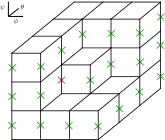
\includegraphics[width=0.4\textwidth]{schemes/StaggeredGrid.pdf}
	\caption{General view of the staggered grid points marked as crosses on top of the collocated cells. The red cross at the position $[i_\psi, i_\theta - \frac{1}{2}, i_\varphi-\frac{1}{2}]$ corresponds to the central cell with index $[i_\psi, i_\theta, i_\varphi]$}
	\label{fig:StaggeredGridOverview}
\end{figure}

In the following work, quantities evaluated at staggered grid points are indicated either by the superscript $stg$ or by a $-\frac{1}{2}$ shift in the index. This means that following notations are equivalent: 
\begin{align*}
	X^{stg}_{[i_\psi,i_\theta,i_\varphi]} &= X_{[i_\psi,i_\theta-\frac{1}{2},i_\varphi-\frac{1}{2}]} &\text{or}&& X^{stg}_{[i_\psi,i_\theta+1,i_\varphi]} &= X_{[i_\psi,i_\theta+\frac{1}{2},i_\varphi-\frac{1}{2}]}
\end{align*}

\subsection{Boundary cells}

Staggered quantities require a different treatment at the domain boundary. In the geometry definition, entire cells belong either to the plasma or to the physical wall. Collocated quantities in the boundary layer are thus always half a cell width away from the wall and boundary conditions are enforced accordingly. For the magnetic vector potential this holds for walls in $\psi$ direction but in $\varphi$ and $\theta$ directions, the staggered grid points are on the tokamak wall for the boundary cells with lowest index and one cell width away at the highest index. For consistency, accuracy and symmetry purposes, the staggered solvable domain shall be either extended by one row of cells at the upper index to include the wall in the solution or or reduced by one row at the lower end. In both cases, the number of collocated and staggered grid points do not match anymore and inhibit all eventual symmetry properties of the matrix in the dual-grid system (\ref{eq:vorticityEquation_electromagnetic_dedimensionalized_implicitEulerSystem}). $A_\parallel$ requires Dirichlet boundary conditions with the value 0 everywhere, thus the solution on the wall is already known and is not needed in the system. Therefore the latter option without the staggered grid points of the lower boundary cell layer is more suitable and has been implemented as depicted in \autoref{fig:StaggeredGridBC}.
\begin{figure}[H]
	\centering
	\includegraphics[width=0.4\textwidth]{schemes/staggeredGridBoundary.pdf}
	\caption{General view of the staggered grid points in the $\theta-\varphi$ plane that are solved in the vorticity equation. Note that at the lower boundaries, collocated fields are included in the system but not their staggered counterparts. }
	\label{fig:StaggeredGridBC}
\end{figure}
In the system (\ref{eq:vorticityEquation_electromagnetic_dedimensionalized_implicitEulerSystem}), some entries for the electric potential $\Phi$ do not have a corresponding magnetic potential $A_\parallel$. To ensure a correct implementation of the system and the stencils that appear in it, a new mask $\chi^{stg}$ describes which cells contain staggered grid points in the solvable domain. It is defined from the original collocated wall mask $\chi$ as: 
\begin{equation}
	\label{eq:def_chi_staggered}
	\chi^{stg}_{[i_\psi,i_\theta, i_\varphi]} = 1 - (1 - \chi_{[i_\psi,i_\theta  ,i_\varphi  ]})
	(1 - \chi_{[i_\psi,i_\theta-1,i_\varphi  ]})
	(1 - \chi_{[i_\psi,i_\theta  ,i_\varphi-1]})
	(1 - \chi_{[i_\psi,i_\theta-1,i_\varphi-1]})
\end{equation}
The value of $\chi^{stg}_{[i_\psi,i_\varphi,i_\theta]}$ is therefore 1 if the staggered grid point of the cell with index $[i_\psi,i_\varphi,i_\theta]$ lies on or in the wall and it is 0 inside the solvable domain.



Another implication for staggered fields occurs at sheath boundaries, where $A_\parallel$ and $j_\parallel$ lie on the domain boundary. For collocated fields, we impose sheath fluxes from the Bohm-Chodura model (see Sec. \ref{sec:boundaryConditions}) on the first cell in the simulation domain. For the magnetic potential $A_\parallel$, the 0-Dirichlet condition is imposed in the concerned cell. For the parallel current $j_\parallel$, we add the sheath current $j_{\text{wall}}$ to any parallel currents tangential to the wall. Indeed, if the sheath boundary is in the $\theta$ direction, the $\varphi$ component of the parallel current remains unaffected and needs to be solved. 



\subsection{Staggered discrete operators}
As the parallel current $j_\parallel$ and the magnetic vector potential $A_\parallel$ are defined on a staggered grid, new stencil operators are needed to be compatible with the electric potential $\Phi$ defined on the collocated grid at the cell centers. 

\subsubsection{Divergence on a parallel vector field}

In \autoref{eq:vorticityEquation_electromagnetic}, the divergence of $j_\parallel$ needs to be calculated at the collocated grid. We thus need a discrete stencil operator 
$$\left[\grad\cdot X^{stg}\vec{b}\right]^{col}_{[i_\psi,i_\theta, i_\varphi]}$$
In \autoref{eq:MetricDivergenceParallel}, the divergence of a parallel vector field has been introduced. We consider a collocated cell as in \autoref{fig:StaggeredGridOverview}. The flux $\pdv{\left(J X b^\theta\right)}{u^\theta}$ is then the difference between the inflow and the outflow through the two cell faces facing the $\theta$ axis. We want to calculate these fluxes from the flux $F^{X,in} = JXb^\theta$ of the staggered field $X$ known at the crosses in the schematic. We further assume that the inflow to the central collocated cell is the mean of the fluxes at the red cross and at the green cross right to it:
\begin{align*}
	F_{[i_\psi,i_\theta, i_\varphi]}^{X,\theta} &= \frac{1}{2}\left(F_{[i_\psi,i_\theta-\frac{1}{2}, i_\varphi-\frac{1}{2}]}^{X,\theta} + F_{[i_\psi,i_\theta-\frac{1}{2}, i_\varphi+\frac{1}{2}]}^{X,\theta} \right) \\
	&= J_{[i_\psi,i_\theta-\frac{1}{2}, i_\varphi-\frac{1}{2}]}X_{[i_\psi,i_\theta-\frac{1}{2}, i_\varphi-\frac{1}{2}]}b_{[i_\psi,i_\theta-\frac{1}{2}, i_\varphi-\frac{1}{2}]}^\theta + J_{[i_\psi,i_\theta-\frac{1}{2}, i_\varphi+\frac{1}{2}]}X_{[i_\psi,i_\theta-\frac{1}{2}, i_\varphi+\frac{1}{2}]}b_{[i_\psi,i_\theta-\frac{1}{2}, i_\varphi+\frac{1}{2}]}^\theta
\end{align*}

If one of the two staggered points lies on the domain boundary, it is not included in the flux calculation and consequently the factor $1/2$ is dropped. \\

This numerical calculation can be performed for all in- and outflows in $\theta$ and $\varphi$ directions, leading to the final form of the numerical form of the staggered divergence stencil: 
\begin{equation}
	\label{eq:NumericalStaggeredDivergenceStencil}
	\left[\grad\cdot X^{stg}\vec{b}\right]^{col}_{[i_\psi,i_\theta, i_\varphi]} = \frac{1}{J_{[i_\psi,i_\theta, i_\varphi]}} \left(F_{[i_\psi,i_\theta, i_\varphi]}^{X,\theta}-F_{[i_\psi,i_\theta+1, i_\varphi]}^{X,\theta}+F_{[i_\psi,i_\theta, i_\varphi]}^{X,\varphi}-F_{[i_\psi,i_\theta, i_\varphi+1]}^{X,\varphi}\right)
\end{equation}

\subsubsection{Parallel gradient}

In \autoref{eq:vorticityEquation_electromagnetic}, another operator is needed to represent the gradient of $A_\parallel \vec{b}$ on the staggered grid.
$$\left[\grad_\parallel X^{col}\right]^{stg}_{[i_\psi,i_\theta, i_\varphi]}$$
According to \autoref{eq:MetricParallelGradient}, its numerical evaluation is quite straight-forward: 
\begin{align}
	\label{eq:NumericalStaggeredParallelGradientStencil}
	\left[\grad_\parallel X^{col}\right]^{stg}_{[i_\psi,i_\theta, i_\varphi]} =& \frac{1}{2}\left(X_{[i_\psi,i_\theta, i_\varphi]}-X_{[i_\psi,i_\theta-1, i_\varphi]}\right)b_{[i_\psi,i_\theta-\frac{1}{2}, i_\varphi-\frac{1}{2}]}^\theta \nonumber \\ +& 
	\frac{1}{2}\left(X_{[i_\psi,i_\theta, i_\varphi]}-X_{[i_\psi,i_\theta, i_\varphi-1]}\right)b_{[i_\psi,i_\theta-\frac{1}{2}, i_\varphi-\frac{1}{2}]}^\varphi
\end{align}

If any of the used $X$ happens to lie inside the boundary, it is eliminated from the stencil. \\

The staggered divergence and parallel gradient stencils already existed in a hidden form in the original SOLEDGE implementation as part of the parallel Laplacian operator on collocated fields, which first computes the parallel gradient leading to intermediate staggered results and then applies the divergence operator on these staggered intermediate results.

\subsubsection{Perpendicular Laplacian}

Finally, \autoref{eq:vorticityEquation_electromagnetic} requires the perpendicular Laplacian on the staggered grid to link $j_\parallel$ and $A_\parallel$.

$$\left[\Delta_{\perp}X^{stg}\right]^{stg}_{[i_\psi,i_\theta, i_\varphi]}$$

In the scheme proposed by G\"{u}nter et al. \cite{Gnter2005ModellingOH}, this operation is performed in two steps: first the perpendicular gradient is evaluated on $X^{stg}$ which produces an intermediate collocated vector field $\vec{Y}^{col}$ whose divergence leads to the final staggered result. \autoref{eq:MetricPerpendicularDiffusion} includes all needed metrics to achieve this operation. To better understand the final divergence operation, we must imagine a cell centered around the point where the perpendicular Laplacian is required, depicted in \autoref{fig:StaggeredCell}. We then need to calculate the fluxes $F^{Y,i}$ across all six faces. The metric and diffusion coefficients $JD(g^{ij}-b^ib^j)$ are also required at the faces and we obtain them by taking their average on the closest collocated points. In poloidal and toroidal directions two collocated points shown in green in \autoref{fig:StaggeredFluxTheta} and \autoref{fig:StaggeredFluxPhi} are sufficient but in radial direction we need to consider eight points around the face to calculate the correct coefficients. \\

\begin{figure}[H]
	\centering
	\begin{subfigure}[b]{0.24\textwidth}
		\centering
		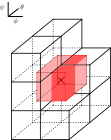
\includegraphics[width=1\textwidth]{schemes/BoundingBoxStaggeredPoint.pdf}
		\subcaption{Cell boundaries \\ for the staggered \\ grid point}
		\label{fig:StaggeredCell}
	\end{subfigure}
	\begin{subfigure}[b]{0.24\textwidth}
		\centering
		\includegraphics[width=1\textwidth]{schemes/BoundingBoxFluxPsiDiffPerp.pdf}
		\subcaption{Relevant faces \\ for the outflow face \\ in $\psi$-direction} 
		\label{fig:StaggeredFluxPsi}
	\end{subfigure}
	\begin{subfigure}[b]{0.24\textwidth}
		\centering
		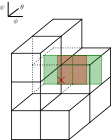
\includegraphics[width=1\textwidth]{schemes/BoundingBoxFluxThetaDiffPerp.pdf}
		\subcaption{Relevant faces \\ for the outflow face \\ in $\theta$-direction} 
		\label{fig:StaggeredFluxTheta}
	\end{subfigure}
	\begin{subfigure}[b]{0.24\textwidth}
		\centering
		\includegraphics[width=1\textwidth]{schemes/BoundingBoxFluxPhiDiffPerp.pdf}
		\subcaption{Relevant faces \\ for the outflow face \\ in $\varphi$-direction} 
		\label{fig:StaggeredFluxPhi}
	\end{subfigure}
	
	\caption{Depiction of the relevant cell faces to calculate fluxes of a staggered field at coordinate index $[i_\psi, i_\theta-\frac{1}{2}, i_\varphi-\frac{1}{2}]$}
	\label{fig:StaggeredPerpendicularLaplancianCellSurfaces}
\end{figure}

The perpendicular Laplacian can thus be succintly written in term of the fluxes in and out of the staggered red cell:
\begin{align}
	\left[\Delta_{\perp}X^{stg}\right]^{stg}_{[i_\psi,i_\theta, i_\varphi]} =& \frac{1}{J_{[i_\psi,i_\theta-\frac{1}{2}, i_\varphi-\frac{1}{2}]}}\left(F^{Y,\psi}_{[i_\psi+\frac{1}{2},i_\theta-\frac{1}{2}, i_\varphi-\frac{1}{2}]} - F^{Y,\psi}_{[i_\psi-\frac{1}{2},i_\theta-\frac{1}{2}, i_\varphi-\frac{1}{2}]}\right. \nonumber \\ 
	&\left.+ F^{Y,\theta}_{[i_\psi,i_\theta, i_\varphi-\frac{1}{2}]} - F^{Y,\theta}_{[i_\psi,i_\theta-1, i_\varphi-\frac{1}{2}]}+ F^{Y,\varphi}_{[i_\psi,i_\theta-\frac{1}{2}, i_\varphi]} - F^{Y,\varphi}_{[i_\psi,i_\theta-\frac{1}{2}, i_\varphi-1]}\right) 	\label{eq:NumericalStaggeredPerpDiffStencil}	
\end{align}

If any of the staggered cell faces touches the domain boundary in any form, the corresponding flux is excluded from the divergence operator. It only remains to calculate the fluxes $F^{Y,i}$. The metric and diffusion coefficients at all faces have already been described and are represented by the term $\xi^{ij}=JD(g^{ij}-b^ib^j)$. We then can express the fluxes as: 
$$ F^{Y,i} = \xi^{ij}\pdv{X}{u^j} $$
The remaining gradient must use $X^{stg}$ at staggered points in the domain. If $[ijk]$ stands for any permutation of the staggered indices $[i_\psi,i_\theta-\frac{1}{2},i_\varphi-\frac{1}{2}]$ we always have a flux of the kind:
\begin{align*}
	F^{Y,i}_{i-\frac{1}{2},jk} &= \xi^{ii}\left(X^{stg}_{ijk}-X^{stg}_{i-1,jk}\right) \\
	&+ \frac{1}{4}\xi^{ij}\left(X^{stg}_{i,j+1,k}-X^{stg}_{i,j-1,k}+X^{stg}_{i-1,j+1,k}-X^{stg}_{i-1,j-1,k}\right) \\
	&+ \frac{1}{4}\xi^{ik}\left(X^{stg}_{i,j,k+1}-X^{stg}_{i,j,k-1}+X^{stg}_{i-1,j,k+1}-X^{stg}_{i-1,j,k-1}\right)
\end{align*}

If any of the field points $X$ lie in or on the domain boundary, it is not considered in the stencil and the factor $\frac{1}{4}$ is changed to $\frac{1}{3}$.

\subsection{Discretization around the X-point}
\label{ssec:DiscretizationXPt}

The staggered grid has direct implications on the estimation of fluxes around mesh singularities: while for regular fields, every cell around the X-point has well-defined neighbors (see Fig. \ref{fig:CenteredXpoint}), radial fluxes in and out of staggered cells directly cross the X-point (see Fig. \ref{fig:StaggeredXpoint}). They affect the perpendicular Laplacian operator on $A_\parallel$ in Ampere's law (Eq. \ref{eq:MagneticPotential}), advection on $j_\parallel$ in Eq. \ref{eq:advectionJpara}, and the anomalous perpendicular diffusion $\mathcal{D}_\perp$. To cope with the ill-defined cell faces, fluxes across the X-point are forced to 0 by Neumann-like boundary conditions. Neighbors of the involved cells must be defined separately from the regular cells with the same index. \newline

\begin{figure}[H]
	\centering
	\begin{subfigure}[t]{0.39\textwidth}
		\centering
		\includegraphics[width=1\textwidth]{schemes/XpointCentered.png}
		\subcaption{View of centered cells}
		\label{fig:CenteredXpoint}
	\end{subfigure}
	\begin{subfigure}[t]{0.39\textwidth}
		\centering
		\includegraphics[width=1\textwidth]{schemes/XpointStaggered.png}
		\subcaption{View of staggered cells}
		\label{fig:StaggeredXpoint}
	\end{subfigure}
	\caption{ Sketches of the mesh around the X-point. For centered cells (a), 8 cells touch the X-point at a corner. For staggered cells (b), the X-point is located at the radial face of 4 cells, effectively modifying the shape of the cells to pentagons. Fluxes across the involved faces are hence ill-defined. }
	\label{fig:XpointDiscretization}
\end{figure}



\section{Time discretization}

The model uses an explicit time discretization for the advection terms and an implicit one for the diffusive terms. In turbulence simulations, we limit ourselves to timescales slower than the cyclotronic frequency $\omega_C$. This applies to all advection phenomena, as well as to friction, pressure, and energy source terms, which can then comfortably be solved explicitly in time. \newline

However, ionization/recombination processes, resistive and viscous effects from the Spitzer-Härm model, and electron inertia involve much faster dynamics that would massively constrain the allowed timestep size. Therefore, these terms are solved implicitly. To reduce numerical complexity, they can be decoupled and solved sequentially for the density, the parallel velocity, the temperature, and finally the potentials. 

\subsection{Explicit Runge-Kutta solver}

%Unlike the advection terms, the update of the electric potential in the vorticity equation \ref{eq:ElectrostaticVorticityEquation} requires an implicit numerical scheme, for which we use the 1-st order implicit Euler method. The electric potential $\Phi^{n+1}$ at the next time integration step $n+1$ is the solution of the following system:

%\begin{equation}
%	\label{eq:OldVorticityEquation_timeDiscrete}
%	\left(\frac{1}{\delta t}\tilde{\Delta}_\perp + \sigma_\parallel\Delta_\parallel \right)\Phi^{n+1} = \frac{1}{\delta t}\tilde{\Delta}_\perp\Phi^{n} - \vec{\grad}\cdot\vec{F}_{\Omega} + \vec{\grad}\cdot\left(\zeta\vec{\grad}_\perp\Omega\right) + \tilde{RHS}
%\end{equation}

%This system turns out to be very expensive to solve because of the high anisotropy between the perpendicular and parallel Laplacian components in the  matrix on the left-hand side.\\

\subsection{Implicit-explicit VSIMEX solver}

The time discretization is based on a variable stepsize implicit-explicit scheme (VSIMEX) \cite{wang2008variable}, associating explicit time discretization for the advection terms and an implicit one for the diffusive terms. In turbulence simulations, we limit ourselves to timescales slower than the cyclotronic frequency $\omega_C$. This applies to all advection phenomena, as well as to friction, pressure, and energy source terms, which can then comfortably be solved explicitly in time. \newline


This multi-step method is implemented for orders 1 to 3, and the timestep is updated such that fluxes and velocities in the simulation domain match a targeted CFL value. \newline



\section{Initialization at Restart}
\subsection{Electron Inertia}
Use the steady-state Ohm's law from the exisiting profile in $\Phi$.

\subsection{Parallel Magnetic Vector Potential}
Solve for the steady-state Ampère's law with the now available profile in $\j_\parallel$. Creation of a new solver class for this purpose.

\section{Implicit Numerical Treatment}

\subsection{Parallel diffusion operator with flutter}
\label{ssec:3DGunter}

In the magnetostatic setting, the parallel diffusion operator on $v_i$ and $T_\alpha$ can be solved independently on each flux surface in a 2D system on the $\theta - \varphi$ plane. The scheme developed by Günter et al. \cite{gunter2005} has proven well-suited to solve the 2D parallel Laplacian equations with minimized numerical spread for highly anisotropic problems. For an operator of the type $\nabla \cdot (\kappa \nabla_\parallel \circ \mathbf{b} )$, parallel gradients are first calculated in cell corners with finite differences and then used in the fluxes across each cell face to get the divergence. The corners where gradients are calculated are shown in Figure \ref{fig:Gunter2D}. This scheme is particularly effective if the poloidal and toroidal components $b^\theta$ and $b^\varphi$ of the contravariant magnetic unit vector in the curvilinear metric have similar magnitudes. This is usually enforced through careful mesh generation. \newline

However, with flutter (Sec. \ref{sec:flutter}), magnetic flux surfaces are no longer aligned to the $\theta - \varphi$ plane because of the new radial component $b^\psi$. As a consequence, all independent 2D problems across flux surfaces are now coupled into a single 3D problem. For the parallel diffusion solver, a first approach would be to extend the above scheme by calculating gradients in the 3D corners of our cells. However, the new component $b^\psi$ is a pure fluctuation, which is therefore expected to be much smaller than $b^\theta$ or $b^\varphi$ and can even vanish locally. This results in significant spurious numerical diffusion in the radial direction of equilibrium gradients. To prevent this diffusion, and still properly capture radial flutter gradients, only crossed derivatives $b^\theta b^\psi$ and $b^\varphi b^\psi$ as well as the principal radial diffusion $b^\psi b^\psi$ use gradients evaluated at 3D corners, while the equilibrium diffusion remains aligned to the $\theta - \varphi$ plane. Examples of the gradients used in this new scheme are shown in Figs. \ref{fig:Gunter3D_theta} and \ref{fig:GunterD_psi}. The new discretization stencil then corresponds exactly to the equilibrium 2D stencil in the limit $b^\psi=0$. \newline

\begin{figure}[!h]\centering
	\begin{subfigure}[t]{0.32\textwidth}
		\centering
		\includegraphics[width=\textwidth]{schemes/Gunter2D.png}
		\caption{ Gradients for the $\theta$-flux in the electrostatic setting }
		\label{fig:Gunter2D} 
	\end{subfigure}
	\begin{subfigure}[t]{0.32\textwidth}
		\centering
		\includegraphics[width=\textwidth]{schemes/Gunter3D_theta.png}
		\caption{ Gradients for the $\theta$-flux in the electromagnetic setting   }
		\label{fig:Gunter3D_theta} 
	\end{subfigure}
	\begin{subfigure}[t]{0.32\textwidth}
		\centering
		\includegraphics[width=\textwidth]{schemes/Gunter3D_psi.png}
		\caption{ Gradients for the $\psi$-flux in the electromagnetic setting   }
		\label{fig:GunterD_psi}
	\end{subfigure}
	\caption{Sketches showing the calculation of gradients for the parallel diffusion scheme. It shows the position where the different gradients are calculated that are relevant for a flux across the cell face with a solid line. Green and red arrows symbolize gradients in the equilibrium and in the radial direction, respectively.}
	\label{fig:GunterStencils_flutter}
\end{figure}


\subsection{Electromagnetic vorticity system}

The newly introduced fields $j_\parallel$ and $A_\parallel$ are solved implicitly along with the electric potential $\Phi$. As we face a coupled system that connects all points in the domain, direct solvers such as PASTIX are not suitable, especially for fine 3D meshes. We instead prefer to use iterative solvers available in the the PETSc or HYPRE libraries. For the original vorticity system, the Stabilized version of the Biconjugate Gradient method (BiCGStab) along with the Geometric Algebraic Multigrid (GAMG) preconditionner proved to be very efficient and it is desirable to use them on the new systems. This section describes some special numerical features in the construction of the system to facilitate the convergence of the above iterative scheme. \autoref{ssec:equilibrationBLockMatrices} introduces specific row and column scaling to equilibrate the blocks in the new system and \autoref{ssec:StaggeredFieldsMatrix} describes how to handle staggered fields to be compatible with the iterative scheme.

\subsubsection{Expression for the coupled system}

With the values for $n_e$ and $T_e$ known at time-step $n+1$, the vorticity equation (Eq. \ref{eq:VorticityEquation}) corresponds to a 3D costly system involving $\Phi$, $j_\parallel$, and $A_\parallel$. To solve it efficiently, the $j_\parallel$ advection and perpendicular diffusion are treated explicitly, allowing the integration of Ohm's law into the vorticity equation and Ampère's law. Then, at time-step $n+1$, the following dimensionless system coupling the two potentials $\Phi$ and $A_\parallel$ must be solved: \newline

\begin{align}
	\begin{pmatrix}
		\label{eq:implicitSytem}
		\nabla \cdot \left[ D_\perp \nabla_\perp \circ \right] + \nabla \cdot \left[ D_\parallel \nabla_\parallel \circ \mathbf{b} \right] & 
		\frac{\beta_0}{\delta t} \nabla \cdot \left[ D_\parallel \circ \mathbf{b} \right] \\
		D_\parallel \nabla_\parallel \circ &
		\frac{\beta_0}{\delta t} D_\parallel \circ - \nabla \cdot \left[ \nabla_\perp \circ \right]
	\end{pmatrix}
	\begin{pmatrix}
		\Phi^{n+1} \\ A_\parallel^{n+1}
	\end{pmatrix} 
	= \nonumber \\
	\begin{pmatrix}
		\nabla \cdot \left[ D_t j^{n}_\parallel \mathbf{b} \right] + \text{RHS}^\Phi \\
		D_t j^{n}_\parallel + \text{RHS}^{A_\parallel}
	\end{pmatrix}
\end{align}

with $D_\perp = \frac{m_i n_i}{B^2 \delta_t}$, $D_\parallel = \frac{1}{\eta_\parallel + \mu}$, $D_t = \frac{\mu}{\eta_\parallel + \mu}$, and $\mu = m_e / (m_u n_e \delta_t)$ accounting for electron inertia effects. The parameter $\delta t$ derives from the integration scheme and is equal to the time-step in the case of a first-order implicit Euler scheme. \newline

Since $\eta_\parallel \propto T_e^{-1.5}$, the parallel resistivity $\eta_\parallel$ is often a small parameter that leads to strong anisotropy between the perpendicular and parallel Laplacian operators. However, the electron inertia term, being implemented in the current solver, acts as an upper limit for the parallel diffusion coefficient, which is expected to improve the matrix conditioning as $\eta_\parallel$ approaches zero. This is in contrast to the original electrostatic model from \cite{Bufferand2021}. \newline


\subsubsection{Equilibration of the Matrix Blocks}
\label{ssec:equilibrationBLockMatrices}
The matrices in the electromagnetic model \autoref{sec:DedimensionalizedElectromagneticModelS3X} can be decomposed in 2x2 or 3x3 block matrices that apply on the respective fields $\Phi$, $A_\parallel$ and/or $j_\parallel$. Apart of the use of dedimensionalized quantities, no effort was made so far to ensure that the blocks are roughly of the same order of the magnitude, which is important for the condition number of the matrix, nor that the matrix is diagonally dominant, which is generally a desirable feature for fast convergence of iterative schemes. \\
In the following bits, we introduce some column $c_X$ and row $r_X$ scaling factors that are specific to the blocks $X$ of the matrix such that the above conditions are fullfilled as well as possible. To ensure a correct solution, the row scaling factor $r_X$ must be applied to the corresponding entry in the RHS vector and as a matter of fact, in the original vorticity matrix, we already have $r_\Phi = J$ the metrical Jacobian from \autoref{ssec:MetricCurvilinearCoordinates} to remove the effect of different mesh sizes in the domain on the discrete Laplacian operators. The column scaling factors $c_X$ must be taken care of when retrieving the fields from the numerical solution and it is strongly recommended to apply them to the initial guess for the iterative scheme. \\ 
Some exisiting algorithms optimize the scaling task such as ---cite---. However, they all require an expensive matrix analysis phase that must be repeated regularly since the matrix changes with the progress of the simulation. Therefore, we use the knowledge about the construction of the matrix blocks to define sufficiently good scaling factors. \\
In the system with electron inertia \autoref{eq:vorticityEquation_Elect	ronInertia_dedimensionalized_matrix}


\subsubsection{Staggered Fields in the Matrix}
\label{ssec:StaggeredFieldsMatrix}
The GAMG multigrid solves the system on different coarser levels by restricting the matrix and the RHS vector and then interpolates the solution back to the finer levels. In the new system, two consecutive entries belong to different fields, which makes the whole restriction-interpolation task obsolete from the very first level since neither the solution nor the matrix entries are similar between neighbours. In general, PETSc takes care of multiple fields in a coupled system if one defines a block size (in our case either 2 or 3) that indicates GAMG how to match corresponding entries.vim  However, as seen in \autoref{ssec:SpatialDiscretization}, the fields $A_\parallel$ and $j_\parallel$ are defined on a staggered grid in poloidal and toroidal directions as opposed to the centered field for $\Phi$. For the system it means that at each wall in negative directions (at the left target and for non-axisymmetric geometries), a line and column for $\Phi$ exists but not for the two other fields. This in turn is problematic for GAMG as the blocks are globally defined and two different fields would again end up together and the total system size might even not be a multiple of the blocksize (2 resp. 3), which at all prevents the initialization of the preconditioner. \\


For the parallel diffusion on the electric potential $\nabla \cdot \left[ D_\parallel \nabla_\parallel \Phi \mathbf{b} \right]$ with flutter, we do not use the stencil introduced in Sec. \ref{ssec:3DGunter}. To avoid numerical difficulties and the appearance of unphysical modes, the discretization of this term needs to be consistent with the parallel gradient and divergence operators in the same system. Since the grid for $A_\parallel$ and $j_\parallel$ is only staggered in the $\theta$ and $\varphi$ directions, we do not know them in the radial corners from Figs. \ref{fig:Gunter3D_theta} and \ref{fig:GunterD_psi}. Instead, the discrete diffusion operator is defined as the combination of the operators for the gradient and the divergence. It involves two neighbors on both radial sides, so the resulting stencil is less compact but consistent with the remaining system. Note that in cases without flutter ($b^\psi = 0$), the diffusion operator exactly corresponds to Günter's scheme \cite{gunter2005} because the staggered fields are known at the position of the green gradients in Fig. \ref{fig:GunterStencils_flutter}. \newline



	\chapter{Verification and Validation}
\section{Verification by the Method of manufactured solutions}
To ensure the correctness of the newly implemented system with the magnetic vector potential $A_\parallel$, a test model has been set up with the method of manufactured solutions (MMS) \cite{ManufacturedSolution}. This allows to directly compare the numerical and analytic solutions and therefore validate the implementation and verify the order of convergence of the numerical operators. 

\subsection{Test system}
The MMS test model is a fraction of a torus with a circular cross-section with an inner radius of 0.48m, an outer radius of 2.72m and a simulated plasma edge width of 0.64m. An example of the 3D mesh geometry is shown in \autoref{fig:MMSModelScheme}. To test the information exchange between zones in the model topology from \autoref{ssec:SpatialDiscretization}, each coordinate direction is split in two zones totaling to 8 zones.

\begin{figure}[H]
	\centering
	\begin{subfigure}[b]{0.4\textwidth}
		\centering
		\includegraphics[width=1\textwidth]{schemes/torturedGrid_r_phi_view.png}
		\subcaption{Top view of the $\psi-\varphi$ plane \\ \textit{the two bands correspond to \\ the poloidal angles $0$ and $\pi$}}
		\label{fig:MMSModelTorturedTopView}
	\end{subfigure}
	\begin{subfigure}[b]{0.4\textwidth}
		\centering
		\includegraphics[width=1\textwidth]{schemes/torturedGrid_r_theta_view.png}
		\subcaption{View of a cross-section of the torus in the $\psi-\theta$ plane \\ \textit{The cross-section is at $\varphi=0$}}
		\label{fig:MMSModelTorturedCrossSection}
	\end{subfigure}	
	\caption{Distorted MMS mesh geometry with $N=20$ cells per dimension on a 3rd of a torus}
	\label{fig:MMSModelScheme}
\end{figure}

In the MMS geometry, $\psi$ denotes the radius of the tube and $R$ the radius of the entire torus. If $aR_0=1.6$ is the distance of the tube center to the torus center, we have:
$$  R = aR_0 + \psi\cdot\cos(\theta) $$
Together with the poloidal coordinate $\theta\in[0,2\pi]$ and the toroidal coordinate $\varphi\in[0,2\pi/N_{div}]$ where $1/N_{div}$ is the considered fraction of the torus, each point in the domain is uniquely described by the curvilinear coordinates $[\psi,\theta,\varphi]$. 
We can define some $\vec{P} = [X,Y,Z]^T$ in a cartesian basis of the 3D domain:

\begin{align*}
	X &= R\cos(\varphi) &  Y &= \psi\cdot\sin(\theta)  &  Z &= R\sin(\varphi)
\end{align*} 
In this setting, the basis vectors of the curvilinear coordinates from \autoref{ssec:MetricCurvilinearCoordinates} can be calculated analytically. The covariant basis vectors are:
\begin{align*}
	\vec{e}_\psi &= \pdv{\vec{P}}{\psi} = \begin{bmatrix} \cos(\theta)\cos(\varphi) \\ \sin(\theta) \\ \cos(\theta)\sin(\varphi) \end{bmatrix} & \vec{e}_\theta &= \pdv{\vec{P}}{\theta} = \begin{bmatrix} -\psi\sin(\theta)\cos(\varphi) \\ \psi\cos(\theta) \\ -\psi\sin(\theta)\sin(\varphi) \end{bmatrix} & \vec{e}_\varphi &= \pdv{\vec{P}}{\varphi} = \begin{bmatrix} -Z \\ 0 \\ X \end{bmatrix}
\end{align*}
We can further calculate the metric coefficients:
$$ g_{ij} = \vec{e}_i\cdot\vec{e}_j
= \begin{bmatrix}
	1 & 0 & 0 \\ 0 & \psi^2 & 0 \\ 0 & 0 & R^2
\end{bmatrix} \qquad \text{and} \qquad J = \sqrt{\det[g_{ij}]} = \psi R$$
 
As generally required by S3X, the magnetic field is axisymmetric and thus does not depend on the toroidal coordinate $\varphi$. By construction, it only has a poloidal and a toroidal component but no radial component, which are given in \autoref{eq:MMSMagneticField}.

\begin{equation}
	\label{eq:MMSMagneticField}
	\begin{cases}
		B_\theta = \frac{1}{aR}\Psi_0 & \text{poloidal magnetic field}  \\
		B_\varphi = \frac{R_0}{R}B_0 & \text{toroidal magnetic field}
	\end{cases}
\end{equation}

The magnetic field parameters are chosen such that the ratio of toroidal over poloidal magnetic field strength is $aR_0B_0/\Psi_0 = 12$. 
Tests have been performed on various mesh geometries in the scope of S3X from a perfectly regular grid with equally spaced cells in all coordinate directions to the distorted mesh depicted above. As the program can be either executed in a 2D or 3D mode with adapted stencils and geometry calculations, MMS tests have been developed for both scenarios.

\subsection{Analytic solution}

We are interested in the vorticity system on the electric potential $\Phi$ and the parallel magnetic vector potential $A_\parallel$. We postulate that their analytic form is: 
\begin{align}
	\Phi =& \Phi_0 \left(1 + 0.1 \cos(\theta)\cos(\frac{\varphi}{N_{div}})\sin(2\pi \frac{\psi-\psi_{min}}{\psi_{max} - \psi_{min}}) \right) \\
	A_\parallel =& A_{\parallel,0} \left(1 + 0.1 \cos(\theta)\cos(\frac{\varphi}{N_{div}})\sin(2\pi \frac{\psi-\psi_{min}}{\psi_{max} - \psi_{min}}) \right)
	\label{eq:MMSAnalyticFormPhiAPara}
\end{align}

A similar expression is chosen for the densities $n_{i/e}$ and temperatures $T_{i/e}$ that also contribute to the vorticity equation. The entire form of the test equation is:

\begin{align}
	&\begin{cases}
		\partial_t\vec{\grad}\cdot\left(\frac{m_in_i}{B^2}\vec{\grad}_\perp\Phi\right) + \vec{\grad}\cdot\sigma_\parallel \left(\grad_\parallel\Phi\vec{b}+\partial_t A_\parallel\right) &= \partial_t \Omega_\pi + \vec{\grad}\cdot\sigma_\parallel\left( + \frac{T_e}{e}\grad_\parallel \log(n_e)\vec{b} + \frac{1.71}{e}\grad_\parallel T_e\vec{b}\right)  - S^{MMS}_\Phi \\
		\qquad \vec{\grad}\cdot\left(\vec{\grad}_\perp A_\parallel\vec{b}\right) - \mu_0 \sigma_\parallel \left( \grad_\parallel \Phi + \partial_t A_\parallel\right)&= -\mu_0 \sigma_\parallel \left(\frac{T_e}{e}\grad_\parallel \log(n_e) + \frac{1.71}{e}\grad_\parallel T_e\right) - S^{MMS}_{A_\parallel}
	\end{cases} \nonumber \\
	&\Omega_\pi = \vec{\grad}\cdot\left(\frac{m_i}{Z_iB^2}\vec{\grad}_\perp[nT]\right)
	\label{eq:MMSTestSystem}
\end{align}

The main difference to the original system of equations in \autoref{eq:vorticityEquation_electromagnetic} are the MMS source terms $S^{MMS}_\Phi$ and $S^{MMS}_{A_\parallel}$. They contain the analytic evaluation of all other time-independant terms in the respective line of the equation. The derivatives on curvilinear coordinates can be calculated analytically with the metric theory discussed in \autoref{ssec:MetricCurvilinearCoordinates}. Boundary conditions are enforced by a penalty method on the boundary cell layer where the two quantities are set to their analytic expression. The MMS system is initialized with the analytic expressions for $\Phi$ and $A_\parallel$ in \autoref{eq:MMSAnalyticFormPhiAPara} and uniquely the vorticity equation is solved for one timestep. We are in a steady state, so the numerical solution after the first timestep should be equal to the initial state. \\
One drawback of a steady state system is that time derivatives are always assumed to vanish and terms such as $\Omega_\pi$, the perpendicular Laplacian of $\Phi$ or the divergence of $A_\parallel$ are not confronted to their analytic form. To catch these terms, we add the vorticity $\Omega$ to the MMS system and include it in the subsequent analysis. It is initialized with its analytic form:
$$ \Omega = \Omega_\pi + \vec{\grad}\cdot\left(\frac{m_in_i}{B^2}\vec{\grad}_\perp\Phi\right) + \vec{\grad}\cdot\sigma_\parallel A_\parallel $$
and then calculated numerically after the first timestep. This allows to compare a numerical and an analytic form of the vorticity and hence all terms in \autoref{eq:MMSTestSystem}.

\subsection{Order of convergence}
- \\
- \\
- \\
Describe \\
- \\
- \\
- \\
\begin{figure}[H]
	\centering
	\begin{subfigure}[b]{0.49\textwidth}
		\centering
		\includegraphics[width=1\textwidth]{schemes/err_rel_vortAParaSystem_grid2_2D.png}
		\subcaption{2D system}
		\label{fig:MMSTorturedVortAPara2DConvergence}
	\end{subfigure}
	\begin{subfigure}[b]{0.49\textwidth}
		\centering
		\includegraphics[width=1\textwidth]{schemes/err_rel_vortAParaSystem_grid2_3D.png}
		\subcaption{3D system}
		\label{fig:MMSTorturedVortAPara3DConvergence}
	\end{subfigure}
	\caption{Relative error between the initial plasma and the solution after one timestep. The $x$-axis indicates the number of points per zone in each direction, the total number of points is thus $N_{tot}^{3D} = 8\cdot X^3$ (resp. $N_{tot}^{2D} = 4\cdot X^2$). The dashed lines indicate the slope of the ideal 2nd order convergence}
	\label{fig:MMSTorturedVortAParaConvergence}
\end{figure}
- \\
- \\
this beautiful graph \\ - \\ - \\ Thanks.


\section{Linear Analysis}

.... 
\subsection{Pure advection}
A first step to verify the correct physical behaviour of the simulation would be to investigate the plasma advection equations. \\
For this objective we set up a simplistic plasma model on a rectangular 2D SLAB topology. Periodic boundary conditions in all directions allow to properly observe wave propagation without any inference at the domain boundaries. In an isothermal hydrogen plasma without source terms and drifts, the governing equations then simplify to:

\begin{align}
	\partial_t n_i + \vec{\grad}\cdot\left(n_i\vec{u}_i\right) &= 0 \label{eq:AdvectionLinearAnalysis_ionMass} \\
	n_e &= n_i \label{eq:AdvectionLinearAnalysis_quasiNeutrality} \\
	\partial_t \left(m_in_iu_\parallel\right) + \vec{\grad}\cdot\left(m_in_iu_\parallel u_i\right) &= -2T_e\vec{\grad}_\parallel n_e \label{eq:AdvectionLinearAnalysis_parallelMomentumBalance}
\end{align}

In this simple plasma, only the density and the velocity evolve over time and depend on each other. The electric potential $\Phi$ can also be computed and observed, but it does not interfere with the system because the parallel electric field in the momentum balance \autoref{eq:AdvectionLinearAnalysis_parallelMomentumBalance} is calculated from the electron pressure gradient $E_\parallel = (\vec{\grad}_\parallel p_e + R_e) / n_e$. \\

To perform the linear analysis of the system, we assume that field variables such as the velocity or density respect some Fourier solution as sum of several wave modes with respective amplitudes $\tilde{X}_{\omega,k_\perp,k_\parallel}$:
\begin{equation}
	 X = \bar{X} + \hat{X} = X_0 + \sum\tilde{X}_{\omega,k_\perp,k_\parallel}e^{i(-\omega t + k_\perp \psi + k_\parallel \theta)} \label{eq:FourierModeSolution}
\end{equation}

Electron and ion density are identical because of the quasi-neutrality assumption in \autoref{eq:AdvectionLinearAnalysis_quasiNeutrality}. Since we do not consider any drifts the radial component $u_\psi$ of the velocity vector vanishes. Further, the mean density is $\bar{n}=n_0$ while the mean velocity $\bar{u}_\theta$ is zero. Because we are only interested in a first order approximation of the solution, we neglect all higher-order mixed fluctuating terms. Thus, \autoref{eq:AdvectionLinearAnalysis_ionMass} and \autoref{eq:AdvectionLinearAnalysis_parallelMomentumBalance} transform to:

\begin{align*}
	&&-i\omega\hat{n} + i\bar{n}k_\parallel\hat{u}_\theta + i\bar{u}_\theta k_\parallel\hat{n} &= 0 &\Leftrightarrow&& \hat{u}_\theta &= \frac{\omega}{n_0k_\parallel}\hat{n} \\
	&& -i\omega m_i \left(\bar{n}\hat{u}_\theta + \bar{u}_\theta\hat{n}\right) + im_ik_\parallel\left(2\bar{n}\bar{u}_\theta\hat{u}_\theta + \bar{u}_\theta^2\hat{n}\right) &= -2iT k_\parallel\hat{n}	&\Leftrightarrow&&  \hat{u}_\theta &= \frac{2T k_\parallel}{m_in_0\omega}\hat{n}
\end{align*}

Both are combined to obtain a dispersion relation for the frequency $\omega$:
\begin{align}
	&& \frac{\omega}{n_0k_\parallel} &= \frac{2T k_\parallel}{m_in_0\omega} 
	&\Leftrightarrow&& \omega &= \pm\sqrt{\frac{2T}{m}}k_\parallel \label{eq:AdvectionLinearAnalysis_dispersionRelation}
\end{align}

It is apparent that both solutions for $\omega$ are real therefore non-decaying waves traveling with the speed of sound $c_s = \sqrt{2T/m}$ appear. The perpendicular wave mode does not contribute to the equation so a 1D system along the poloidal axis is sufficient to simulate the behaviour. Both the electron and the ion density are initialized with one sinusoidal perturbation and \autoref{fig:AdvectionSLAB_densityEvolution} shows their evolution. The electron velocity in \autoref{fig:AdvectionSLAB_velocityEvolution} responds to this initial excitation with a shifted standing wave with same frequency. 

\begin{figure}[H]
	\centering
	\begin{subfigure}[b]{0.32\textwidth}
		\centering
		\includegraphics[width=1\textwidth]{schemes/AdvectionSLAB_1D_timeplot_ne.png}
		\subcaption{Evolution of the density \\ \ }
		\label{fig:AdvectionSLAB_densityEvolution}
	\end{subfigure}
	\begin{subfigure}[b]{0.32\textwidth}
		\centering
		\includegraphics[width=1\textwidth]{schemes/AdvectionSLAB_1D_timeplot_ve.png}
		\subcaption{Evolution of the velocity \\ \ }
		\label{fig:AdvectionSLAB_velocityEvolution}
	\end{subfigure}
	\begin{subfigure}[b]{0.32\textwidth}
		\centering
		\includegraphics[width=1\textwidth]{schemes/AdvectionSLAB_FFT.png}
		\subcaption{time Fourier transform of the density and velocity}
		\label{fig:AdvectionSLAB_FFT}
	\end{subfigure}
	\caption{Evolution of the 1D SLAB system with 64 cells in poloidal direction over 10000 timesteps with the RK4 scheme. For a better readability only parts of the graphs are represented}
	\label{fig:AdvectionSLAB}
\end{figure}

The system is initialized with one wavemode along the "poloidal" length of $L=100$m so the wavenumber here is $k_\parallel = 2\pi / L \approx 0.0628$. The plasma temperature is kept constant at $T = 100$eV and the mass of a deuterium atom equals to $m_i \approx 3.34\cdot 10^{-27}$kg, so we can expect a system frequency of $\omega\approx 978$Hz from the dispersion relation in \autoref{eq:AdvectionLinearAnalysis_dispersionRelation}. This corresponds precisely to the main frequency peak in \autoref{fig:AdvectionSLAB_FFT} and thus acoustic waves appear in the system as expected. The smaller peaks at higher frequency modes are however not physical and are likely due to numerical noise as their appearance highly depends on the spatial and temporal resolution and their intensity increases for longer simulations. 


\subsection{Electrostatic case}
Before plunging into the vorticity equation with $A_\parallel$ it may be interesting to discuss whether the correct behaviour is actually observed in the original electrostatic implementation. For that we reduce the system to the bare minimum set of equations that involve the electric potential $\Phi$. Neglecting all kind of transport equations and source phenomena remains the following simple equation on $\Phi$: \\
\begin{equation}
		\partial_t\grad\cdot\left[\frac{m_in_i}{B^2}\grad_\perp\Phi\right] = -\grad\cdot\sigma_\parallel\grad_\parallel\Phi \label{eq:AdvectionSLAB_PHI}
\end{equation}

whose simple dispersion relation reads, assuming that $k_\perp \ne 0$:
\begin{align}
	\omega &= -\frac{B^2\sigma_\parallel}{m_in_i}\frac{k_\parallel^2}{k_\perp^2}i &\Rightarrow&& \lambda &= \frac{B^2\sigma_\parallel}{m_in_i}\frac{k_\parallel^2}{k_\perp^2}
\label{eq:AdvectionSLAB_dispersionRelation}
\end{align}

As $\omega$ is a pure negative complex number, we do not expect any oscillations but an exponential decay of the solution. All points in the domain decay with 
\begin{align}
	\Phi(t) = \Phi_0 e^{-\lambda t} + C \label{eq:electrostaticSLABdecay}
\end{align} 
where the decay rate $\lambda$ is the negative imaginary part of $\omega$ and $\Phi_0$ relates to the initial distribution of the electric potential.

The time integration of this system can only be performed by solving the implicit system because there is no direct expression for the time derivative of $\Phi$. Further, the electric potential $\Phi$ appears only in perpendicular and parallel Laplacian operators. Together with the periodic boundary conditions in all directions, one degree of freedom remains and the solution of $\Phi$ can only be calculated up to a constant $C$. To make the system invertible, it is thus necessary to add some term to the system. One simple approach is to fix (or ground) $\Phi$ to a set value $\Phi^G$ at one point $[i_\psi^G, i_\theta^G]$ in the domain. This defines the free parameter $C$ and $\Phi(t)$ at all points converges to $\Phi^G$. 

\begin{figure}[H]
	\centering
	\begin{subfigure}[b]{0.34\textwidth}
		\centering
		\includegraphics[width=1.\textwidth]{schemes/electrostaticSLAB_1_Phi.png}
		\subcaption{Initial $\Phi(\psi,\theta)$ \\ \ }
		\label{fig:electrostaticSLAB_initialProfile_PHI}
	\end{subfigure}
	\begin{subfigure}[b]{0.34\textwidth}
		\centering
		\includegraphics[width=1.\textwidth]{schemes/electrostaticSLAB_35_Phi.png}
		\subcaption{$\Phi(\psi,\theta)$ after 350 timesteps \\ \ }
		\label{fig:electrostaticSLAB_endProfile_PHI}
	\end{subfigure}
	\begin{subfigure}[b]{0.30\textwidth}
		\centering
		\includegraphics[width=0.95\textwidth]{schemes/Electrostatic_analysis_different_k_para_k_perp.png}
		\subcaption{Estimated decay rates for different wavemodes}
		\label{fig:electrostaticSLAB_decayRateFit}
	\end{subfigure}
	\caption{Evolution of the 2D electrostatic SLAB system with 64 cells in radial and poloidal direction over 10000 timesteps with the implicit Euler scheme. The system is grounded at the center of the domain to $\Phi^G = 0$V.}
	\label{fig:electrostaticSLAB}
\end{figure}

The uniform decay can be clearly seen between \autoref{fig:electrostaticSLAB_initialProfile_PHI} and \autoref{fig:electrostaticSLAB_endProfile_PHI}. It remains to investigate whether the observed attenuation matches the expected decay rate $\lambda$. A Fourier transformation as to determine oscillatory modes for the standing acoustic waves in the previous section is not of great help here, instead we use a non-linear least squares to fit the time evolution of $\Phi(t)$ at an arbitrary point in the domain except the grounded point. We fit the parameters $\Phi_0$, $\lambda$ and $C$ from \autoref{eq:electrostaticSLABdecay} to the simulation data and compare the hence estimated $\lambda$ to the theoretical decay rate for the given initial wave. \autoref{fig:electrostaticSLAB_decayRateFit} shows that there is a strong agreement between the theoretical and fitted decay rates for a large array of domain configurations. The wavenumbers $k_\parallel$ and $k_\perp$ were modified by changing the poloidal respectively the radial size of the domain with always the first wave mode spanning the entire domain. We can safely claim that the original electrostatic implementation produces the expected physical behaviour.

\subsection{Electromagnetic case}
While acoustic waves are characteristic for a physical medium, Alfvén waves dominate oscillations of ions within a magnetic field. The motion occurs in direction of the magnetic field lines where the ion mass accounts for the inertia and the magnetic field tension for the restoring wave force. The Alfvén wave group velocity for a species $i$ is given by:

\begin{equation}
	v_A = \frac{B}{\sqrt{m_in_i\mu_0}} \label{eq:AlfvenGroupVelocity}
\end{equation}

With the new parallel magnetic vector potential $A_\parallel$ into the vorticity \autoref{eq:vorticityEquation_electromagnetic} Alfvén waves should appear in the simulation and the aim of this section is to prove their existence. We follow the same approach as in the previous section for the electrostatic case and reduce the system to the strict necessary minimum and keep following equations: 
\begin{align}
	\partial_t\grad\cdot\left[\frac{m_in_i}{B^2}\grad_\perp\Phi\right] &= \grad\cdot\sigma_\parallel\left(-\grad_\parallel\Phi-\partial_tA_\parallel\right) \label{eq:electromagneticSLAB_PHI} \\
	\Delta_{\perp}A_\parallel &= -\mu_0\sigma_\parallel\left(-\grad_\parallel\Phi-\partial_tA_\parallel\right) \label{eq:electromagneticSLAB_APara}
\end{align}

We ignore any kind of advection phenomena thus all densities $n_{i/e}$ and temperatures $T_{i/e}$ keep their initial uniform distributions their gradients vanish. If we perform the linear analysis of the remaining system we get following relation for \autoref{eq:electromagneticSLAB_PHI}:
\begin{align*}
	&&i\frac{m_in_i}{B^2}k_\perp^2\omega\hat{\Phi} &= \sigma_\parallel k_\parallel^2\hat{\Phi}-\sigma_\parallel k_\parallel\omega\hat{A}_\parallel \\
	&\Leftrightarrow& \hat{A}_\parallel &= \left(\frac{k_\parallel}{\omega} - i\frac{m_in_ik_\perp^2}{\sigma_\parallel B^2k_\parallel}\right)\hat{\Phi}
\end{align*}

and for \autoref{eq:electromagneticSLAB_APara}:
\begin{align*}
	&&-k_\perp^2\hat{A}_\parallel &= i\mu_0\sigma_\parallel k_\parallel\hat{\Phi} - i\mu_0\sigma_\parallel\omega\hat{A}_\parallel \\
	&\Leftrightarrow&\hat{A}_\parallel &= \frac{\mu_0\sigma_\parallel k_\parallel}{\mu_0\sigma_\parallel\omega + i k_\perp^2}\hat{\Phi}
\end{align*}

If we combine both expressions we can relate the frequency to the parallel and perpendicular wave modes:
\begin{align}
	&& \frac{k_\parallel}{\omega} - i\frac{m_in_ik_\perp^2}{\sigma_\parallel B^2k_\parallel} &= \frac{\mu_0\sigma_\parallel k_\parallel}{\mu_0\sigma_\parallel\omega + i k_\perp^2} \nonumber \\
	&\Leftrightarrow& i\frac{m_in_ik_\perp^2\omega}{\sigma_\parallel B^2k_\parallel^2} &= 1- \frac{\mu_0\sigma_\parallel\omega}{\mu_0\sigma_\parallel\omega + i k_\perp^2} \nonumber \\
	&\Leftrightarrow& \omega^2 + i\frac{k_\perp^2\omega}{\mu_0\sigma_\parallel} &= \frac{B^2}{m_in_i\mu_0}k_\parallel^2 \nonumber
\end{align}
We find the square of the Alfvén group velocity \ref{eq:AlfvenGroupVelocity} as a factor before the parallel wave number. There is an additional imaginary term in the dispersion relation which depends on the perpendicular wave number and adds some damping to the system. Let us call $\gamma = 1/(\mu_0\sigma_\parallel)$ the associated damping coefficient. The dispersion relation can then be rewritten to: 

\begin{equation}
	\omega^2+i\gamma k_\perp^2\omega-v_A^2k_\parallel^2=0 \label{eq_electromagneticSLAB_fullDispersionRelation}
\end{equation} 

If we transform the system back to the time domain, we expect a damped solution for the potentials $\Phi$ and $A_\parallel$ of the form \cite{waveDispersionRelation}:

\begin{equation}
  X = X_0 + \hat{X}e^{-\lambda t}e^{i\left(-\omega_0 t + k_\perp \psi + k_\parallel \theta\right)} \label{eq:electromagneticSLAB_underdampedSolution}
\end{equation}

where the decay rate $\lambda$ contains the imaginary part and the oscillation frequency $\omega_0$ the real part of $\omega$. \\

In the case that $\gamma k_\perp^2 > 2v_Ak_\parallel$, the frequency $\omega$ is purely imaginary and the system decays to the mean value $X_0$ with the rate:
\begin{equation}
	\lambda = \frac{\gamma}{2}k_\perp^2 \pm \sqrt{\frac{\gamma^2}{4}k_\perp^4-v_A^2k_\parallel^2} \label{eq:electromagneticSLAB_overdampedDecayRate}
\end{equation} 

If on the other hand $\gamma k_\perp^2 < 2v_Ak_\parallel$, the frequency $\omega$ has both a real and an imaginary part. The decay rate is then:
\begin{equation} 
	\lambda = \frac{\gamma}{2}k_\perp^2 \label{eq:electromagneticSLAB_underdampedDecayRate}
\end{equation}
and the system frequency: 
\begin{equation} 
	\omega_0 = \pm\sqrt{v_A^2k_\parallel^2 - \frac{\gamma^2}{4}k_\perp^4} \label{eq:electromagneticSLAB_underdampedFrequency}
\end{equation}

In the case that the damping term is much smaller than the oscillatory term (if for instance the parallel wave mode dominates over the perpendicular one), $\omega$ is a real number and the system frequency only depends on the Alvén group velocity and we should be able to observe pure Alfvén waves.
$$ \omega_0 = v_A k_\parallel$$

In \autoref{eq:electromagneticSLAB_overdampedDecayRate} and \autoref{eq:electromagneticSLAB_underdampedFrequency} we see that there are two possible solution for the decay rate respectively the oscillation frequency. This does not conflict with our assumed wave solution which has been defined in \autoref{eq:FourierModeSolution} as the sum of several Fourier modes and each solution here contributes to one mode. 
 
As in the electrostatic case from the previous section, the just described system is not invertible and $\Phi$ is defined up to a constant. Grounding the potential in one single point is however not a suitable solution here because it deteriorates the condition number of the vorticity matrix past solvability. Instead two other approaches will be followed to check if simulations can reproduce the expected physical behaviour. 

%\subsubsection{Grounded line}
%One approach is to set the potential not in one but in several points to a fixed value. The potential in the remaining domain then distributes according to this value and the whole system becomes solvable. Numerically, this is achieved by replacing the row of the matrix corresponding to the grounded point by a single 1 on the diagonal and the matching term in the RHS vector by the desired value for $\Phi$. This operation is equal to enforcing Dirichlet boundary conditions in radial direction if $\Phi$ is grounded at all points with index $i_\psi^G$. 
%
%\begin{figure}[H]
%	\centering
%	\begin{subfigure}[b]{0.45\textwidth}
%		\centering
%		\includegraphics[width=.98\textwidth]{schemes/44_APara.png}
%		\subcaption{$A_\parallel(\psi,\theta)$ at the timestep 440\\ \ }
%		\label{fig:electromagneticSLAB_initialProfile_A}
%	\end{subfigure}
%	\begin{subfigure}[b]{0.45\textwidth}
%		\centering
%		\includegraphics[width=1\textwidth]{schemes/excitedSLAB_2D_timeplot_A.png}
%		\subcaption{Time evolution of $A_\parallel(t)$ in the lower left corner of the domain}
%		\label{fig:electromagneticSLAB_evolution_A}
%	\end{subfigure}
%	\caption{Snapshot of an electromagnetic SLAB simulation on a domain with $N_\psi=32$ and $N_\theta=64$ grid points. All point at the radial center with $i_\psi^G$ are grounded.}
%	\label{fig:electromagneticGroundedSLAB_system}
%\end{figure}
%
%In the simulations with a grounded line, the initial wave solution has been applied to the vorticity field $\Omega$ to prevent steep gradients and instabilities if it was done on $\Phi$ directly. Very soon, the two potentials $\Phi$ and $A_\parallel$ respond to this initial excitation and a wave profile appears as depicted in \autoref{fig:electromagneticSLAB_initialProfile_A}. The line of grounded points in the middle of the domain however breaks the wave which then smoothly lines up with the equilibrium point $\Phi_0 = 0V$ and $A_{\parallel,0} = 0Tm$ around the grounded line. At this point it may be emphasized that only the electric potential $\Phi$ is grounded, but as both potential fields are strongly coupled the grounded line affects $A_\parallel$ equally. We thus have a wave that is guided between two poloidal grounded lines (remember that the domain is periodic in radial direction) so by construction the system cannot account for radial dynamics. If we consider a point that is furthest away from the grounded line (e.g. any point on the domain boundary in the example above) we might still be able to observe some expected physical behaviour. At first glance, if we track $A_\parallel$ in one point over time as in \autoref{fig:electromagneticSLAB_evolution_A}, a decaying oscillation appears which is in line with the here dominant underdamped regime. 	
%
%First we investigate the underdamped scenario by opposing simulation results to the expected damping rates $\lambda$ and frequencies $\omega_0$. As for the previous electromagnetic we fit the four free parameters in \autoref{eq:electromagneticSLAB_underdampedSolution} to simulation data with a nonlinear least squares method. With 1000 sample points we get a high fitting fidelity with a relative standard deviation of the order of $10^{-9}$ and the difference if the fit is performed on $\Phi$ or $A_\parallel$ has about the same magnitude. 
%
%\begin{figure}[H]
%	\centering
%	\begin{subfigure}[b]{0.45\textwidth}
%		\centering
%		\includegraphics[width=.98\textwidth]{schemes/groundedSLABunderdampedFiterrors_k_para_fixed.png}
%		\subcaption{Poloidal mode fixed to $k_\parallel = $}
%		\label{fig:electromagneticSLAB_errorGrounded_kPara_fixed}
%	\end{subfigure}
%	\begin{subfigure}[b]{0.45\textwidth}
%		\centering
%		\includegraphics[width=1\textwidth]{schemes/groundedSLABunderdampedFiterrors_k_perp_fixed.png}
%		\subcaption{Radial mode fixed to $k_\perp = 100m^{-1}$}
%		\label{fig:electromagneticSLAB_errorGrounded_kPerp_fixed}
%	\end{subfigure}
%	\caption{Relative error for the fits of the frequency $\omega_0$ and the decay rate $\lambda$ on the evolution of $A_\parallel$ with respect to the expected values in a grounded electromagnetic SLAB simulation on a domain with $N_\psi=32$ and $N_\theta=64$ grid points.}
%	\label{fig:electromagneticSLAB_errorGrounded}
%\end{figure}






%\subsubsection{Diagonal perturbation}
%Another approach that
% 
%\autoref{eq:electromagneticSLAB_PHI} on the potential is then replaced by:
%\begin{equation*}
%	\partial_t\grad\cdot\left[\frac{m_in_i}{B^2}\grad_\perp\Phi\right] + \varepsilon \Phi= \grad\cdot\sigma_\parallel\left(-\grad_\parallel\Phi-\partial_tA\right) + \varepsilon \Phi_e
%\end{equation*}
%
%This addition naturally affects the dispersion relation and we end up with:
%\begin{equation*}
%	\omega^2+\left(i\gamma k_\perp^2 - \frac{B^2\epsilon}{m_in_ik_\perp^2}\right)\omega-v_A^2k_\parallel^2+\frac{v_A^2 \epsilon}{\sigma_\parallel}=0
%\end{equation*}
%
%This eventually changes the previously calculated frequencies and damping rates. For the overdamped case, we get:
%$$ \lambda = \frac{\gamma}{2}k_\perp^2 - \frac{B^2\epsilon}{2m_in_ik_\perp^2} \pm \sqrt{\frac{\gamma^2}{4}k_\perp^4-v_A^2k_\parallel^2}$$


\subsection{Linear transition from Alfvén to thermal electron waves}

In Sec. \ref{sec:edge_DAW}, we introduced drift-Alfvén waves. With the electromagnetic extensions, drift-waves are coupled to higher-frequency modes that transition from the Alfvén to the thermal electron speed and travel along magnetic field lines. These modes are associated with negative growth rate and usually dampen out quite fast. They can however be used to validate the electromagnetic implementation. The thought behind it is that if we reduce the system to suppress drift-waves, and run simulations with a sufficiently temporal resolution, the transition should appear in the SOLEDGE3X simulations. \\

The following simplified model (Eq. \ref{eq:VV_fourFieldModel}) is considered on the electron density $n_e$, parallel current $j_\parallel$, and the potentials $\Phi$ and $A_\parallel$: \newline

\begin{equation}
	\left\{
	\begin{aligned}
		\partial_t n_e &= \frac{1}{e}\nabla \cdot (j_\parallel \mathbf{b}) \\
		j_\parallel + \frac{\sigma_\parallel m_e}{n_e e^2} \partial_t j_\parallel  &= \sigma_\parallel \left( -\nabla_\parallel \Phi - \partial_t A_\parallel + \frac{T_e}{e} \nabla_\parallel \log(n_e) \right) \\
		\nabla \cdot \left[ \frac{m_i n_i}{B^2} \partial_t \nabla_\perp \Phi \right] &= \nabla \cdot (j_\parallel \mathbf{b}) \\
		\Delta_\perp A_\parallel &= -\mu_0 j_\parallel 
	\end{aligned}
	\right.
	\label{eq:VV_fourFieldModel}
\end{equation}

The computational domain is a 3D slab domain with periodic boundary conditions in all directions. The magnetic field is assumed to be constant in the $\theta-\varphi$ plane. The wavenumbers $k_\psi$, $k_\theta$, and $k_\varphi$ are defined by the respective dimensions of the slab. Parallel and perpendicular wavenumbers express as: \newline

\begin{align}
	k_\parallel = b_\theta k_\theta + b_\varphi k_\varphi &&& k_\perp = \sqrt{k_\psi^2 + k_\theta^2 + k_\varphi^2 - k_\parallel^2}
\end{align}

The Alfvén wave speed is given by $v_A = \frac{B_0}{\sqrt{m_u n_e \mu_0}}$ and the electron thermal speed by $v_{th,e} = \sqrt{\frac{e T_e}{m_e}}$. In the zero-resistivity limit, the dispersion relation states that we deal with a complex wave frequency, whose real component is: \newline

\begin{align}
	\label{eq:VV_dispersionRelation}
	\omega_0^2 = \frac{v_A^2}{1 + \frac{m_e}{e^2 \mu_0 n_e} k_\perp^2} k_\parallel^2 + \frac{1}{\frac{n_e \mu_0}{T_0 k_\perp^2} + \frac{1}{v_{th,e}^2}} k_\parallel^2  
\end{align}

From Eq. \ref{eq:VV_dispersionRelation}, we expect a wave in the parallel direction traveling at the Alfvén velocity for small $k_\perp$ and at the thermal electron velocity at high $k_\perp$. In the slab domain, $k_\perp$ is changed by changing the radial dimension of the domain. The results of our numerical simulations perfectly match the predictions by Dudson \cite{Dudson2021} and the numerical results obtained by Stegmeir \emph{et al.} \cite{stegmeir2019} and show the expected transition when $k_\perp$ is varied, Fig. \ref{fig:transitionSLAB}. \newline

\begin{figure}[h]\centering
	\centering
	\includegraphics[width=0.7\textwidth]{schemes/transitionAlfvenThermal.png}
	\caption{Fitted wave frequencies as a function of the perpendicular wave numbers. The lines indicate the theoretical wave frequencies in the electrostatic case with finite electron mass (ES), the electromagnetic case with $m_e = 0$ (EM), and the complete electromagnetic case with electron inertia (ES + EM).}
	\label{fig:transitionSLAB}
\end{figure}




!!!! ALERNATIVE TEXT !!!!!!!
Density perturbations provoke an electromagnetic response. To this effect, we consider a standard four-field model that couples the electron density $n_e$ with the parallel current density $j_\parallel$ and both potentials $\Phi$ and $A_\parallel$. The governing equations now are: 

\begin{align}
	\grad\cdot\left[\frac{m_i n_i}{ B^2}\partial_t\grad^2_\perp\Phi\right] &= \grad\cdot(j_\parallel\mathbf{b}) \\
	\grad^2_\perp A_\parallel &= -\mu_0j_\parallel \\
	\eta_\parallel j_\parallel + \frac{ m_e}{n_ee^2} \partial_t j_\parallel  &= \left(-\grad_\parallel\Phi - \partial_t A_\parallel + T_e\grad_\parallel\log(n_e)\right) \\
	\partial_t n_e &= \frac{1}{e}\grad\cdot (j_\parallel\mathbf{b}) 
	\label{eq:fourFieldModel}
\end{align}

Its complex dispersion relation has a real and an imaginary part indicating the appearance of a decaying wave. 

\begin{equation}
	\label{eq:dispersionRelation}
	\omega_A^2 = \left(\frac{v_A^2}{1 + \frac{m_e}{e^2 \mu_0 n_e} k_\perp^2} + \frac{1}{\frac{n_e \mu_0}{T_0 k_\perp^2} + \frac{1}{v_{th,e}^2}}\right) k_\parallel^2 - \frac{\eta_\parallel^2k_\perp^4}{4\left(\mu_0+\frac{m_e}{e^2n_i}k_\perp^2\right)^2}
\end{equation}

The dispersion relation describes "shear Alfvén waves", according to which perturbations travel along magnetic field lines. In cases with high parallel conductivity, the first term dominates the dispersion relation. We then observe that the relation describes a wave in parallel direction whose velocity is bound by the Alfvén wave speed $v_A = \frac{B}{\sqrt{m_in_i\mu_0}}$ for small $k_\perp$ and by the thermal electron wave speed $v_ {th,e} = \sqrt{\frac{T_e}{m_e}}$ for large $k_\perp$. This is in line with the findings by Dudson et al \cite{Dudson2021} and reflects the need for electron inertia to avoid unphysically large speeds in the upper $k_\perp$ limit.



	
	\part[Impact of Electromagnetic Effects on Plasma Simulations]{Impact of Electromagnetic Effects on Plasma Simulations}
	\label{part:EM_Impact}
	\chapter{Limited Geometry}
\label{chap:analSimulations}

\section{Electromagnetic modes excitation}
\label{sec:anal_DAW_modeExcitation}

As an introduction to simulations with SOLEDGE3X, let us consider the linear behavior of drift-Alfvén waves again. To put later simulation results in perspective, we analyze the impact of electromagnetic terms on drift-wave turbulence within a linearized system. Specifically, we compare the effects of a finite electron mass (EI-inert), electromagnetic induction with electron mass (EM), and electromagnetic induction with both flutter and electron mass (EM-flutter) in comparison to the baseline electrostatic case. The dispersion relation from Eq. \ref{eq:edge_DAWdispersionRelation} is adjusted to each of the four scenarios and solved exactly using the Python library SymPy for symbolic computation. Notably, we use the full dispersion relation without applying the simplifications used when we introduced the linear behavior of the drift-Alfvén system in Sec. \ref{ssec:edge_DAW_dispersionRelation}. To recall, the dispersion relation is given by: 

´\begin{equation}
	\label{eq:anal_DAWdispersionRelation}
	i\left(\rho_{L,e}^2k_\perp^2 + \beta_0\right)\omega^3 + \left(-i\beta_0\omega_* - \frac{\eta_\parallel en_0T_0k_\perp^2}{B^2}\right)\omega^2 - i\omega_s^2\left(\omega_*-\left(1 + \rho_L^2 k_\perp^2\right)\omega\right) = 0
\end{equation}


Given the coupled nature system, there are several complex solutions for $\omega$ for each scenario, where each corresponds to a different mode. In Fig. \ref{fig:anal_modalBehavior}, the real and imaginary components of all modes are plotted as functions of the perpendicular wave number $k_\perp$, with typical parameters for a mid-sized tokamak. The real component $\omega_R$ represents the wave phase frequency, while the imaginary component $\gamma$ describes the growth or damping rate of each mode. A positive $\gamma$ indicates an unstable mode with exponential growth, whereas a negative $\gamma$ corresponds to a stable mode that is damped over time.

\begin{figure}[H]
	\centering
	\begin{subfigure}[t]{0.85\textwidth}
		\centering
		\includegraphics[width=1\textwidth]{schemes/modes_ES.jpg}
		\subcaption{Electrostatic system}
		\label{fig:anal_modesES}
	\end{subfigure}
\end{figure}
\begin{figure}[H]
	\ContinuedFloat
	\centering
	\begin{subfigure}[t]{0.85\textwidth}
		\centering
		\includegraphics[width=1\textwidth]{schemes/modes_ES-inert.jpg}
		\subcaption{Electrostatic system with electron inertia}
		\label{fig:anal_modesEI}
	\end{subfigure}
\end{figure}
\begin{figure}[H]
	\ContinuedFloat
	\centering
	\begin{subfigure}[t]{0.85\textwidth}
		\centering
		\includegraphics[width=1\textwidth]{schemes/modes_EM.jpg}
		%		\includegraphics[width=1\textwidth]{schemes/modes_ES.jpg}
		\subcaption{Electromagnetic system}
		\label{fig:anal_modesEM}
	\end{subfigure}
\end{figure}
\begin{figure}[H]
	\ContinuedFloat
	\centering
	\begin{subfigure}[t]{0.85\textwidth}
		\centering
		\includegraphics[width=1\textwidth]{schemes/modes_EM-flutter.jpg}
		\subcaption{Electromagnetic system with flutter}
		\label{fig:anal_modesFlutter}
	\end{subfigure}
	\caption{Dependency on the perpendicular wavenumber $k_\perp$ of the real and imaginary parts of the all solutions $\omega$ to the dispersion relation \ref{eq:anal_DAWdispersionRelation}. Except for $k_\perp$, all other values derive from: $B = 1$T, $n = 2\cdot10^{19}$m$^{-3}$, $T = 100$eV, $\lambda_p = 0.1$m and $k_\parallel = 0.6$m$^{-1}$. On a pair of graphs, a given color represents the same mode. In the left plots for $\Re{\omega}$, characteristic frequencies of the system are shown for reference ("--" diamagnetic $\omega_*$,"$\cdots$" electron sound $\omega_{s,e}$, "-$\cdot$-" Alfvén $\omega_A$).} 
	\label{fig:anal_modalBehavior}
\end{figure}

In the green curve, we observe the characteristic drift-wave frequency, which initially follows the diamagnetic frequency $\omega_*$ in the lower $k_\perp$ limit and reaches its maximum at $k_\perp \rho_L = 1$, before declining again. When the electron inertia term is introduced, a new mode emerges, starting at a significantly higher frequency before stabilizing at the electron sound frequency $\omega_{s,e} = v_{th,e} k_\parallel$. The introduction of electromagnetic terms governs the behavior of the new modes in the lower $k_\perp$ limit, which are then bounded by the shear Alfvén phase velocity. Qualitatively, the phase frequencies exhibit similar characteristics with or without flutter, with the primary difference being a more pronounced separation between the two modes as they transition from $\omega_A$ to $\omega_{s,e}$ in the pure induction. Overall, the characteristic frequencies of the electromagnetic modes are several orders of magnitude higher than the drift-wave frequency.

Looking at the growth rates associated with the modes, we first observe that drift waves are unstable with strong positive growth rates where the frequency is maximal, consistent with the earlier discussion about drift-wave instabilities. On the other hand, electromagnetic (and electron inertial) modes are very stable, showing strong negative $\gamma$. If one intends to study the growth and propagation of turbulent structures and their global impact, Alfvénic modes will only marginally contribute. It is hence possible to avoid the numerical costs involved with the high-frequency modes without much loss of accuracy.

It is more important to consider the effects of electromagnetic contributions on the drift-wave mode. For this purpose, Fig. \ref{fig:anal_comparisonDW} compares the real and imaginary parts of the drift-wave modes in the three electromagnetic scenarios with those in the electrostatic scenario.

\begin{figure}[H]
	\centering
	\begin{subfigure}[t]{0.45\textwidth}
		\centering
		\includegraphics[width=1\textwidth]{schemes/comparison_DW_real.png}
		\subcaption{Real component}
		\label{fig:anal_comparisonDWreal}
	\end{subfigure}
	\begin{subfigure}[t]{0.45\textwidth}
		\centering
		\includegraphics[width=1\textwidth]{schemes/comparison_DW_imag.png}
		\subcaption{Imaginary component}
		\label{fig:anal_comparisonDWimag}
	\end{subfigure}
	\caption{Relative difference of drift-wave frequency in the electromagnetic scenarios to the reference electrostatic case.} 
	\label{fig:anal_comparisonDW}
\end{figure}

The real part is altered by the electromagnetic additions, but the change of phase frequency will only have a minor impact on production cases. On the other hand, the growth rate increases with electron inertia and even more with electromagnetic induction. Electromagnetic flutter on the other largely mitigates the instabilities, and can even reduce the growth rate observed in electrostatic drift waves.



\section{Slab configurations}
\subsection{Analysis of a plasma blob}
\label{ssec:plasmablob}

The linear analysis from the previous section has only , as characteristic shear Alfvén and thermal electron times are much shorter than the ion cyclotronic time, which underlies the resolution of typical turbulent SOLEDGE3X simulations. Drift Alfvén waves in turn correspond to the impact of inductive electromagnetic effect on the formation of drift waves, where the term $\partial_t A_\parallel$ in Ohm's law modifies the non-adiabatic response of the potential $\Phi$ to parallel fluctuations of the electron pressure $p_e$. To study the these effects on a plasma blob in a slab domain. \newline

We place ourselves in a plasma environment similar to the separatrix region in the diverted TCV simulations from the next Chapter \ref{chap:TCV}. The magnetic field is aligned to the toroidal coordinate with $B_{eq,t} = 1.3$T with a curvature of $1.1$m from the tokamak center, similar to the position of the separatrix at the outer mid-plane in TCV. Limiters are placed at both toroidal ends such that that connection length $L_\varphi = 65$m. A cartesian grid with coordinates $r$ and $z$ discretizes each poloidal plane, allowing radial fluxes out and with periodic boundary conditions in the vertical $z$-direction. The electron temperature is kept constant at $T_e=60$eV, ions are cold and the background density is set to $n_0 = 10^{19}$part/m$^3$. To simplify the study and prevent numerical difficulties at the sheath, we apply Neumann-0 boundary $\partial_\parallel n^{BC} = 0$ on the density and the potential $\Phi$ is fixed to $\Phi^{BC} = \Lambda T_e^{BC}$. This is a major simplification to the typical SOLEDGE3X sheath conditions described in Sec. \ref{sec:S3X_boundaryConditions}. The axisymmetric blob initially takes a Gaussian profile 

\begin{equation}
	n = n_0 \left(1 + \alpha e^{-\left[(r-r_b)^2+(z-z_b)^2\right]/\delta_b}\right)
	\label{eq:blobInitProfile}
\end{equation}

with a blob overdensity $\alpha = 2$ and radius $\delta_b = 1$cm. The blob evolves with curvature and electric drifts, neglecting anomalous perpendicular diffusion and viscous effects. Further, electron inertia effect are neglected with $m_e = 0$. We compare the reference electrostatic case with magnetic induction in the parallel electric field and the full electromagnetic setting including flutter. The simulation results are collected in Fig. \ref{fig:BLOB}. \newline

\begin{figure}[H]\centering
	\centering
	\includegraphics[width=1.\textwidth]{schemes/blob_compare_9_6_microsec.png}
	\caption{Density profiles [part/m³] after 9.6$\mu$s simulated plasma time for the electrostatic (ES), magnetic inductive (EM) and full electromagnetic scenarios (EM-flutter). The first row shows a view of the $R-\varphi$ plane with the maximum density taken along the $Z$ coordinate. The second and third rows show the density on poloidal planes ($R-Z$) at the center of the field lines (1) and in proximity to the sheath (2).}
	\label{fig:BLOB}
\end{figure}

In the center of the domain, drift waves determine the potential $\Phi$ but it is dominated by the sheath in proximity to the limiters. Hence a parallel gradient appears on $\Phi$, which in turn induces a parallel current responsive to inductive electromagnetic effects. As a result, the blob filaments bends along the toroidal direction, with higher advection velocities in the center of the domain than at the sheath. The bending is much more pronounced for the two electromagnetic scenarios, in line with the findings of previous blob studies\cite{lee2015,lee2015electromagnetic,Stepanenko_2020}. On closed field lines, the blob would conserve its axisymmetry and both $j_\parallel$ and $A_\parallel$ would remain 0 throughout the simulation. \newline




\subsection{Generation of drift waves}
\label{ssec:plasmaturbslab}

In the previous section, we examined how a single plasma blob propagates across open field lines. However, this does not account for how the blob appears in the first place. In this second part of the slab study, we investigate the onset of drift waves. We consider the same setting as before but with a background density of $n_0 = 2 \cdot 10^{19}$ part/m$^3$ and isothermal electrons and ions at $T_e = T_i = 50$ eV. Instead of an initial overdensity, we apply a constant particle source of $5 \cdot 10^{22}$ part/s on the core side, at all $R < 1.12$ m. The emergence of drift-wave instabilities for the three scenarios is shown in Fig. \ref{fig:SLABturb}. \newline

\begin{figure}[H]\centering
	\centering
	\includegraphics[width=.95\textwidth]{schemes/slab_source.png}
	\caption{Density profiles [part/m³] at the toroidal center of the slab, at about 32m from both limiters. The snapshots compare the electrostatic (ES), magnetic inductive (EM) and full electromagnetic scenarios (EM-flutter) scenarios after 8, 16 and 24$\mu$s simulated plasma time.}
	\label{fig:SLABturb}
\end{figure}

Initially, the particle source causes the density to build up on the core side of the slab. The radial gradient becomes stronger and soon collapses into drift waves. These waves are particularly pronounced in the electrostatic and electromagnetic inductive models. The term $\partial_t A_\parallel$ in Ohm's law intensifies the turbulent interchange, with plasma filaments reaching much further outward. On the other hand, the electromagnetic model with flutter has a stabilizing effect, producing only a thin turbulent layer at the exit of the source and maintaining a strong gradient at the transition from high- to low-density regions. As more particles are introduced at the source, the pressure differential causes this transition line to bend at scales of the simulation box, while the local gradient remains very steep. \newline

\section{Circular geometry}

\subsection{Simulation set-up}

Flat limiter on the low-field side


\begin{figure}[H]\centering
	\centering
	\includegraphics[width=1\textwidth]{schemes/CIRC_fluctT.jpg}
	\caption{Snapshots of the electron temperature $T_e$ fluctuations}
	\label{fig:CIRC_fluctPHI}
\end{figure}


\subsection{Instability growth rates}

As we restart the simulations from a smooth profile, we can observe the growth of instabilities in the beginning of the simulation. Initially, instabilities will grow linearly until they reach a saturation point, when nonlinear effects kick in. In this first (short) phase, we will be able to verify the tendencies from the analysis of the dispersion relation in Sec. \ref{sec:anal_DAW_modeExcitation}, thus electron inertia has a slight and magnetic induction a strong destabilizing while flutter stabilizes the system. To evaluate the perturbations, we calculate the root mean square (RMS) deviation from the toroidal average in every cell. The global metric is then obtained by averaging the local values over the volume $V$ of the entire domain. 

\begin{equation}
	RMS_X = \frac{1}{V}\int_V \sqrt{\frac{X^2 - \langle X \rangle_\varphi^2}{\langle X \rangle_\varphi^2}}  dV
\end{equation}
	
We compare the RMS for both the ion density and temperature at each timestep where a plasma save is available. 

\subsubsection{Electron inertia}

First, we study the impact of electron inertia. For that, we artificially modify the value of the electron mass from its physical value. The results for the RMS of ion density and temperature are collected in Fig. \ref{fig:CIRC_meScan}. We observe that perturbations grow faster as the electron mass increases, reaching the saturation level earlier. The saturation itself is comparable in both cases. The biggest difference already appears between the cases $0m_e$ and $0.5m_e$, hence adding a finite electron mass has an immediate effect to the original implementation where electrons react instantaneously to the system, even for a small mass. 
 
\begin{figure}[H]\centering
	\begin{subfigure}[t]{0.45\textwidth}
		\centering
		\includegraphics[width=1\textwidth]{schemes/RMSn_meScan.jpg}
		\subcaption{RMS of density $n_i$}
	\end{subfigure}
	\begin{subfigure}[t]{0.45\textwidth}
		\centering
		\includegraphics[width=1\textwidth]{schemes/RMST_meScan.jpg}
		\subcaption{RMS of temperature $T_i$}
	\end{subfigure}
	\caption{Evolution of the the root mean square deviation for different values of $m_e$. The electron mass is artificially increased and the 0 factor corresponds effectively to the electrostatic reference}
	\label{fig:CIRC_meScan}
\end{figure}


\subsubsection{Magnetic induction}

Second, we modify the value of the reference $\beta_0$ that appears in the dimensionless equations for the term $\partial_t A_\parallel$ in the parallel electric field. From a physical standpoint, we actually change the vacuum permeability $\mu_0$ as the reference pressure $n_0T_0$ and magnetic field strength $B_0$ remain unchanged for the rest of the model. All simulations are run with the true value of the electron mass, so the base case $0\beta_0$ is equivalent to the green line in the $m_e$ scan above. In Fig. \ref{fig:CIRC_betaScan}, we observe that perturbations grow faster the stronger $\beta_0$ is. For the case $1\beta_0$, we also included flutter as a dashed line, and we see there that the growth rate is reduced again to levels below the electron inertial case. 

\begin{figure}[H]\centering
	\begin{subfigure}[t]{0.45\textwidth}
		\centering
		\includegraphics[width=1\textwidth]{schemes/RMSn_betaScan.jpg}
		\subcaption{RMS of density $n_i$}
	\end{subfigure}
	\begin{subfigure}[t]{0.45\textwidth}
		\centering
		\includegraphics[width=1\textwidth]{schemes/RMST_betaScan.jpg}
		\subcaption{RMS of temperature $T_i$}
	\end{subfigure}
	\caption{Evolution of the the root mean square deviation for different values of $\beta$. The  is artificially increased and the 0 factor corresponds effectively to the electrostatic with electron inerita. The electron mass for all scenarios is physical (factor 1 in Fig. \ref{fig:CIRC_meScan}).}
	\label{fig:CIRC_betaScan}
\end{figure}

For both the $m_e$ and $\beta_0$ scan, we could see that the linear growth corresponds to the expectations from the linear analysis. As the effects of electron inertia and magnetic induction get stronger, plasma perturbations grow faster and reach their saturation point faster. Note that the saturation levels are similar for all scenarios, so the used RMS metric is not very adapted to analyze the subsequent nonlinear phase of the simulation. \\

The results here can however not be correlated one-to-one to the dispersion relation. In the SOLEDGE3X model, interchange instabilities also contribute to the rise of perturbation, and the simulation was run with the energy conservation equation and hence ion and electron temperature gradients add an additional source of instability. The dispersion relation was calculated without curvature effects and using an isothermal assumption, but the general expected trend is still observed. 








	\chapter{Electromagnetic simulations on a realistic diverted geometry}

To demonstrate the abilities of SOLEDGE3X to perform electromagnetic turbulence simulations of a realistic tokamak geometry, the configuration of the test cases has been inspired by the TCV-X21 benchmark \cite{oliveira2022}. This latter addresses L-mode discharges in TCV with a single lower X-point. The semi-implicit time discretization implemented in this model allows comparisons to be made between the electrostatic and electromagnetic models using the same code. Four cases have therefore been considered here: electrostatic (ES), electrostatic with electron inertia (ES-inert), electromagnetic (EM), and electromagnetic with flutter (EM-Flutter). \newline

\section{Simulation set-up}

The plasma is pure deuterium, and only a quarter-torus with a relatively low resolution of approximately 1.9 million cells has been considered to speed up computations (see the mesh in a poloidal plane in Fig. \ref{fig:TCVmesh}). A constant heat source of 25 kW is applied to both electrons and ions, equating to a full-torus equivalent total Ohmic heating of 200 kW. The external toroidal magnetic field is $B_t = 0.95$ T, and the density at the separatrix is targeted to $7 \cdot 10^{18}$ part/m$^3$. \newline

Since the aim of these preliminary computations was to focus on electromagnetic effects, neutrals have been omitted to speed up the convergence of the solutions. Simulations with a more complete physical model will be performed in a further work, including in particular the latest fluid neutral model \cite{quadri2024} developed for regimes dominated by charge exchanges \cite{horsten2017}. \newline

In all cases, the initial condition is the corresponding 2D transport solution obtained by increased perpendicular diffusion coefficients. \newline

In Fig. \ref{fig:EMsnapshots}, typical poloidal cuts of important plasma fields are shown. The local value of $\beta$ varies between $10^{-3}$ at the hot core boundary, $10^{-4}$ around the separatrix and divertor region, and $10^{-5}$ or lower in the far SOL. Consequently, the flutter perturbation $\tilde{B}$ of the magnetic field remains small compared to the equilibrium field, barely exceeding 0.1\% of $B_t$ on the hot core side of the domain. The advection velocity associated with the flutter is also minimal, contributing to less than 0.1\% of the cross-field transport, dominated by the electric "ExB" drift. \newline

\begin{figure}[H]\centering
	\centering
	\makebox[\textwidth][c]{\includegraphics[width=1.3\textwidth]{schemes/TCVnoNeutrSnapshots.png}}    
	\caption{Simulation snapshots of the full electromagnetic scenario with flutter. The first poloidal plane is shown after 6 ms simulated plasma time on the TCV case. From left to right, the first row shows the ion density $n_i$, the electron temperature $T_e$, the electric potential $\Phi$, and the radial "ExB" drift velocity $v_E^\psi$. The second row shows the parallel magnetic potential $A_\parallel$, the parallel current density $j_\parallel$, the amplitude of the flutter field $\norm{\mathbf{\tilde{B}}}$, and the radial flutter advection velocity $v_{\tilde{b}^\psi}$.}
	\label{fig:EMsnapshots}
\end{figure}




\section{Comparison between the scenarios}

We now compare the impact of the different levels of new physics on the TCV scenario. Since turbulent structures are essentially driven by the electric "ExB" drift, we consider the associated total kinetic energy $E_{ExB} = \frac{1}{2}m_i \int_V n_i \norm{v_E}^2 dV$ to estimate the turbulence level. As shown in Fig. \ref{fig:KE_ExB}, a finite electron mass does not change the energy level with respect to the reference electrostatic scenario. Next, adding magnetic induction with $A_\parallel$ further amplifies the turbulent interchange. This enhancement arises from the increased coupling between the magnetic and electric fields, leading to more instabilities and modified turbulent dynamics. Consequently, turbulent filaments give way to smaller, rounder blobs. Finally, the inclusion of flutter has a stabilizing effect on the turbulence, where fluctuations fall again to the level in the electrostatic case. Nonlinear effects in the parallel current equation, namely from the parallel pressure gradient $\nabla_\parallel p_e$, substantially impact the profiles of $j_\parallel$ and hence the response of the potential $\Phi$. The direct consequence is a modification of the radial electric field and a modified evolution of "ExB" drifts. This does not contradict our previous observation that magnetic advection is negligible with respect to the electric drift. \newline

With a different turbulence level, the heat exhaust is also affected, as shown in Fig. \ref{fig:HeatExhaust}. Without radiative effects, the quasi-totality of the heat leaves the tokamak at two divertor targets. The supplementary radial turbulent transport in the magnetic inductive scenario allows more hot particles to cross the separatrix from the core, which will then eventually reach the divertor. Overall, the heat flux is multiplied by a factor of 10. Electron inertia alone leads to an increase by a factor of 2, despite very similar turbulence levels. This phenomenon needs further investigation. Flutter does not reduce further the heat exhaust as one might expect because it is already very low in the electrostatic case. \newline

\begin{figure}[H]\centering
	\begin{subfigure}[t]{0.45\textwidth}
		\centering
		\includegraphics[width=1\textwidth]{schemes/KE_ExB.png}
		\subcaption{Kinetic energy of the "ExB" drift on D$^+$ ions.}
		\label{fig:KE_ExB}
	\end{subfigure}
	\begin{subfigure}[t]{0.45\textwidth}
		\centering
		\includegraphics[width=1\textwidth]{schemes/heatExhaust.png}
		\subcaption{Total heat exhaust}
		\label{fig:HeatExhaust}
	\end{subfigure}
	\caption{Evolution of the kinetic energy and heat exhaust over time iterations on the turbulent TCV scenario. It indicates the turbulence level and its consequence on the total heat transport.}
	\label{fig:performanceMetric}
\end{figure}

The change in turbulence intensity naturally impacts the mean profiles in Fig. \ref{fig:OMP_profiles}. The most noticeable change affects the electromagnetic inductive scenario, where density and temperature gradients are considerably reduced by the additional radial turbulent transport. Again, the finite electron mass has no significant impact, and the reduced turbulence levels by flutter lead to steeper gradients. At this point, we stress the similarity to the simplified drift wave simulations on slab in Sec. \ref{ssec:plasmaturbslab}, where the gradients from the dense core follow the same pattern. \newline

\begin{figure}[H]\centering
	\begin{subfigure}[t]{0.30\textwidth}
		\centering
		\includegraphics[width=1\textwidth]{schemes/OMP_profiles_e-_n.png}
		\subcaption{Plasma density $n$}
	\end{subfigure}
	\begin{subfigure}[t]{0.30\textwidth}
		\centering
		\includegraphics[width=1\textwidth]{schemes/OMP_profiles_e-_T.png}
		\subcaption{Electron temperature $T_e$}
	\end{subfigure}
	\begin{subfigure}[t]{0.30\textwidth}
		\centering
		\includegraphics[width=1\textwidth]{schemes/OMP_profiles_global_fields_PHI.png}
		\subcaption{Electric potential $\Phi$}
	\end{subfigure}
	\caption{Radial profiles at the outer mid-plane after 6 ms simulated plasma time. These profiles were obtained by averaging simulation data across all 32 toroidal planes and over the last 20 available plasma saves.}
	\label{fig:OMP_profiles}
\end{figure}



\section{Numerical performances}
\label{performances}

In our previous work \cite{tamain2016tokam3x, Bufferand2021} about the electrostatic model, it was pointed out that solving the implicit 3D vorticity operator is the most expensive and tricky operation in the algorithm. Adding new variables inevitably modifies the code's performance. With the rather coarse mesh used in the present work, simulations have been run on 16 nodes with 48 CPUs each on the MARCONI supercomputer operated by CINECA \cite{iannone2018marconi-fusion}. Implicit systems, such as the 3D vorticity operator, have been inverted using the stabilized biconjugate gradient method (BCGS) \cite{vandervorst1992bicgstab} with the generalized algebraic multigrid preconditioner (GAMG) by PETSc \cite{petsc-web-page}. \newline

The overall performance of the code largely depends on how quickly a certain plasma timespan can be calculated. Table \ref{tab:performanceMetric} presents the average simulation time for one timestep, broken down by the cost of each implicit solver. For the vorticity system, we also provide the number of iterations the BCGS needed to match the imposed tolerance ($10^{-8}$), as it relates to the condition number of the matrix. This system has always accounted for a considerable share of the total execution time and was heavily modified with the new electromagnetic model. Finally, the timestep size is provided, as a higher timestep size can compensate a costlier problem because the desired simulation time is reached in fewer iterations. As described earlier in Sec. \ref{sec:EquationDiscretization}, SOLEDGE3X uses a variable timestep scheme to maximize the CFL condition with the calculated fluxes. \newline

\begin{table}[h!]
	\centering
	\makebox[\textwidth][c]{
		\begin{tabularx}{1.13\textwidth}{|X|>{\centering\arraybackslash}p{0.12\textwidth}|>{\centering\arraybackslash}p{0.12\textwidth}|>{\centering\arraybackslash}p{0.12\textwidth}|>{\centering\arraybackslash}p{0.12\textwidth}|>{\centering\arraybackslash}p{0.12\textwidth}|>{\centering\arraybackslash}p{0.12\textwidth}|}
			\hline
			& Total execution time per timestep [ms] & Execution time for the viscosity [ms]  & Execution time for the heat diffusion [ms] & Execution time for the vorticity [ms] & N° of vorticity solver iterations & Timestep size [ns]  \\
			\hline
			\textbf{ES}         & 664  & 61  & 76  & 339  & 80  & 15.6 \\
			\hline    
			\textbf{ES-inert}   & 523  & 61  & 77  & 193  & 32  & 16.4 \\
			\hline    
			\textbf{EM}         & 895  & 63  & 82  & 552  & 60  & 15.9 \\
			\hline    
			\textbf{EM-flutter} & 2019 & 225 & 390 & 1147 & 55  & 16.6 \\
			\hline  
		\end{tabularx}
	}	
	\caption{Numerical metrics on the four TCV scenarios for one timestep. All quantities are averaged over the last 20000 timesteps of the simulation. The execution time refers to the wall-clock time and must be multiplied by the number of used processors (768) to get the actual used CPU time.}
	\label{tab:performanceMetric}
\end{table}

Introducing finite electron mass to the vorticity system significantly reduces the number of BCGS iterations and the overall solve time. This improvement occurs because electron inertia effects dominate Ohm's law, thereby reducing the anisotropy between the perpendicular and parallel Laplacians on $\Phi$ in the electrostatic scenario. This reduction in anisotropy is due to the parallel diffusion coefficient being the conductivity $\sigma_\parallel$ in the electrostatic case, but a finite electron mass $m_e$ imposes an upper limit on it. Adding $A_\parallel$ doubles the size of the matrix and introduces a more complex structure, challenging the solvers and requiring more iterations. Despite the higher complexity, a finite electron mass allows the solver to converge in fewer iterations than in the reference electrostatic case. However, the effective solve time is still worse due to the doubling in system size. Finally, including flutter slightly improves the matrix condition compared to the scenario with only magnetic induction, but the execution time is significantly increased. At first glance, one would expect the solve time to correlate with the number of BCGS iterations as both electromagnetic scenarios solve a coupled 3D system on $\Phi$ and $A_\parallel$. Since flutter introduces the radial direction to parallel gradients, and the coupling terms between the two unknowns are exactly a parallel gradient and a divergence (see Eq. \ref{eq:implicitSytem}), the matrix exhibits a decreased sparsity ratio. This circumstance is further aggravated by the fact that $A_\parallel$ is not staggered in the radial direction, so the radial discrete gradient/divergence operator has a larger stencil width than its poloidal and toroidal counterparts. \newline

The viscosity and heat diffusion solvers are not directly affected by the electromagnetic model, and their solve times are similar for the first three scenarios. Electromagnetic flutter, however, with its radial gradient (again), heavily modifies the parallel diffusion operators and requires solving one global 3D system instead of separate 2D systems on each flux surface (see Sec. \ref{ssec:3DGunter}). This is immediately reflected in the code performance, as both solvers take up to 5 times longer to solve. \newline

In total, electron inertia decreases the computing time with an excellent improvement of the vorticity matrix condition. The magnetic inductive model means slightly higher computational costs, because the implicit vorticity problem doubles in size. Including electromagnetic flutter in the system almost quadruples the execution time compared to the original implementation because the radial parallel gradient complicates both the implicit vorticity and the parallel diffusion problem. The timestep size does not vary considerably between the scenarios and hence has only a limited impact on the overall performance.

	\chapter{Perspectives for Studying Magnetic Ripple}
\label{chap:RippleMagnetic}


\begin{chaptersummarybox}
	The SOLEDGE3X code was adapted to impose external non-axisymmetric perturbations of the magnetic equilibrium. In tokamaks such as WEST, the pronounced toroidal magnetic ripple significantly affects plasma confinement and power exhaust, modulating both the poloidal and toroidal components of the equilibrium field. Using the Biot-Savart law, the ripple field is calculated as a magnetic perturbation on the SOLEDGE3X mesh. It is calulated at every grid point from the current in discretized coil segments:
	\begin{equation*}
		\textbf{B}_{ripple} = \frac{\mu_0}{4\pi}I_c\sum_{i=1}^{N_{c}}\sum_{j=1}^{N_{seg}}\frac{\textbf{d}_{i,j}\cross\left(\textbf{s}_{i,j+1} - \textbf{s}_{i,j}\right)}{\norm{\textbf{d}_{i,j}}^3}
	\end{equation*}	
	Preliminary simulations of a WEST scenario reveal a "snake-skin" heat deposition pattern in the divertor region, consistent with experimental observations from infrared cameras.
\end{chaptersummarybox}

\newpage


Developments performed in the scope of this thesis can be useful for applications other than electromagnetic effects on plasmas. In transport mode with large perpendicular diffusion coefficients, a regime where drifts and turbulent scales are not solved, modulations of the magnetic field can have an external source. Because of the toroidal locality of toroidal field coils, the equilibrium magnetic field itself is not axisymmetric, a phenomenon usually referred to as "magnetic ripple". This chapter describes how the implementation of fluctuating magnetic fields in the framework of flutter can be used to simulate perturbations of the equilibrium magnetic field. Sec. \ref{sec:ripple_intro} motivates the study of magnetic ripple, Sec. \ref{sec:rippleCalculation} describes its calculation from an existing axi-symmetric equilibrium and Sec. \ref{sec:ripple_applicationWEST} demonstrates its application on the divertor heat exhaust in WEST. The chapter is slightly adapted from the paper "Implementation of a non-axisymmetric magnetic configuration in SOLEDGE3X to simulate 3D toroidal magnetic ripple effects: Application to WEST", submitted to Nuclear Materials and Energy in the special issue for the PSI-26 conference held in May 2024, Marseille.


\section{Motivation for simulating magnetic ripple}
\label{sec:ripple_intro}

Power exhaust is a major concern in magnetic fusion research. Accurately predicting the heat load on the divertor plates is essential for the design and operation of current and future tokamaks. Estimates for the International Thermonuclear Experimental Reactor (ITER), the most powerful device currently under construction, indicate maximum local heat loads close to material limits\cite{gunn2017surface}.For this reason it is important to study transport of heat and particle fluxes in present experiments, coupling the experimental analysis with a modelling effort  with dedicated numerical tools. \newline

Experiments conducted on the tungsten environment steady-state tokamak (WEST) at CEA in Cadarache, France\cite{bucalossi2022}, have demonstrated that the heat deposition on the divertor targets is not uniform in the toroidal direction. A "snake skin" pattern (see Fig. \ref{fig:IR_WEST}), with alternating local maxima, appears on the inner and outer divertor targets. Reconstructions from infrared camera images exhibit a considerable difference between peaks and lows along a target line. These variations correlate with the disposition of the toroidal magnetic field coils, which locally modify the field lines and amplitude. This effect is known as magnetic ripple\cite{tani1981effect}, and it is particularly pronounced on WEST, where the 18 coils cause strong variations in the amplitude of the magnetic field $\textbf{B}$. For example, fast ions trapped in the toroidal magnetic field ripple have been found to be responsible for significant power losses\cite{moiraf2023optimization}. Moreover, it is important to determine the impact of this toroidal modulation on impurity transport, in particular on tungstene contamination of the core\cite{diGenova2021modelling}. \newline

For heat exhaust studies, SOLEDGE3X is used in "transport" mode, where cross-field transport is approximated with effective diffusion coefficients. It allows simulations to run until convergence on large machines like ITER\cite{rivals2022soledge3x} or JT-60SA\cite{deGianni2024}. Applications of this code include studies on impurity transport\cite{Ciraolo2021}, heat exhaust\cite{rivals2022impact}, and detachment regimes in the divertor\cite{yang2023control}. \newline


\begin{figure}[H]\centering
	\centering
	\includegraphics[width=0.48\textwidth]{schemes/IR_WEST_ripple.jpg}
	\caption[Infrared camera view of the divertor target, taken from \cite{bucalossi2022}]{Infrared camera view of the divertor target, taken from \cite{bucalossi2022}. Red zones correspond to hot regions with high heat deposition. One can see the "snake skin" pattern, where the maximal intensity alternates between the inner and outer strike points.}
	\label{fig:IR_WEST}
\end{figure}

In its current form, SOLEDGE3X can address 2D and 3D axisymmetric configurations as well as 3D non axisymmetric wall geometries\cite{diGenova2023thesis}, but still requires a 3D axisymmetric magnetic field. Therefore, toroidal variations of the magnetic field due to ripple could not be taken into account. Moreover, matching simulation results to experimental data is made difficult by the toroidal locality of Langmuir probes and their consequent susceptibility to ripple effects. Recent developments in the turbulence model have introduced electromagnetic effects\cite{dull2024introducing}, where magnetic field lines are perturbed by fluctuations of the magnetic vector potential. In this paper, we demonstrate that the new implementations can be used not only for plasma-induced perturbations but also for external perturbations of the axisymmetric magnetic field. This paves the way for ripple simulations in SOLEDGE3X and will be applied to a WEST scenario in this paper. 

\section{Generation of a non-axisymmetric magnetic configuration}
\label{sec:rippleCalculation}

The SOLEDGE3X framework is capable of addressing magnetic configurations with singularities at one or more X-points. Constructed by a combination of a toroidal field, $\textbf{B}_t$, and a poloidal field, $\textbf{B}_{pol}$, the expression for the magnetic field is:

\begin{equation}
	\textbf{B}_{axi} = \textbf{B}_t + \textbf{B}_{pol} = F\grad{\varphi} + \grad{\Psi}\cross\grad{\varphi} \label{eq:axiSymBfield}
\end{equation}

where $\varphi$ represents the toroidal angle. The toroidal field $\textbf{B}_t$ is derived from a toroidal flux $F$ and $\textbf{B}_{pol}$ from a poloidal flux function $\Psi$. For high numerical accuracy, the meshing in SOLEGE3X is aligned to magnetic flux surfaces, treating singularities with a multi-domain decomposition shown in Fig. \ref{fig:WESTmesh} \newline 

\begin{figure}[H]\centering
	\centering
	\includegraphics[width=0.48\textwidth]{schemes/WESTmesh.png}
	\caption[Exemplary SOLEDGE3X mesh for a WEST single-null geometry ]{Exemplary SOLEDGE3X mesh for a WEST single-null geometry }
	\label{fig:WESTmesh}
\end{figure}

On top of this axisymmetric basis, we calculate the ripple perturbation of the magnetic field induced by the toroidal distribution of the toroidal field coils. For that, we simplify each coil to a single, circular wire. We first discretize each of the $N_{c}$ coils into $N_{seg}$ segments. For every cell in the SOLEDGE3X grid, we then calculate the magnetic field associated with the coils using the Biot-Savart law:

\begin{equation}
	\textbf{B}_{ripple} = \frac{\mu_0}{4\pi}I_c\sum_{i=1}^{N_{c}}\sum_{j=1}^{N_{seg}}\frac{\textbf{d}_{i,j}\cross\left(\textbf{s}_{i,j+1} - \textbf{s}_{i,j}\right)}{\norm{\textbf{d}_{i,j}}^3}
\end{equation}

where the coil current $I_c$ corresponds to the nominal coil current times the number of wire turns in a coil, $\textbf{s}_{i,j}$ represents the start and end locations of each coil segment, and $\textbf{d}_{i,j}$ is the vector from each mesh point to the segment center. To avoid accounting for the axisymmetric component of the magnetic field twice, we define the perturbation field as the toroidal fluctuations of the ripple field:


\begin{equation}
	\textbf{B}_{pert} = \textbf{B}_{ripple} - \left<\textbf{B}_{ripple}\right>_\varphi
\end{equation}


Together with the axisymmetric part from Eq. \ref{eq:axiSymBfield}, the equilibrium magnetic field as applied to the simulation is given by:

\begin{equation}
	\textbf{B} = \textbf{B}_{axi} + \textbf{B}_{pert}
\end{equation}

\begin{figure}[H]
	\centering
	\begin{subfigure}[t]{0.3\textwidth}
		\centering
		\includegraphics[width=1\textwidth]{schemes/rippleBphi.png}
		\subcaption{toroidal component $B_{pert}^\varphi$ }
		\label{fig:Bpert_phi}
	\end{subfigure}
	\begin{subfigure}[t]{0.3\textwidth}
		\centering
		\includegraphics[width=1\textwidth]{schemes/rippleBpsi.png}
		\subcaption{radial component $B_{pert}^\psi$ }		
		\label{fig:Bpert_psi}
	\end{subfigure}
	\begin{subfigure}[t]{0.3\textwidth}
		\centering
		\includegraphics[width=1\textwidth]{schemes/rippleBtot.png}
		\subcaption{amplitude of the field $\norm{\textbf{B}_{pert}}$}
	\end{subfigure}
	\caption[Top views of the perturbated field $\textbf{B}_{pert}$ on the WEST tokamak at the mid plane]{Top views of the perturbated field $\textbf{B}_{pert}$ on the WEST tokamak at the mid plane. The black dots indicate the position of the toroidal field coils. The  amplitude of the perturbated field remains much smaller than the axisymmetric component, whose amplitude ranges around 1T.}
	\label{fig:Bpert_fields}
\end{figure}

This strategy is now applied to compute the magnetic field ripple for the WEST tokamak, with the coil parameters described in Tab. \ref{tab:coilParameters}. The ripple has a twofold impact on the magnetic equilibrium. A toroidal perturbation field, as shown in Fig. \ref{fig:Bpert_phi}, modifies $\textbf{B}_t$ with local maxima located at the coils' positions and minima midway between two coils. The perturbation vanishes at $\pi/2$ and $3\pi/2$ of a ripple period. Conversely, the radial perturbation in Fig. \ref{fig:Bpert_psi} vanishes at the coils and midway, and modifies the poloidal field $\textbf{B}_{pol}$.

\begin{table}[H]
	\centering
	\begin{tabular}{|c||c|c|}
		\hline
		Number of coils & $N_c$ & 18 \\
		\hline
		Major coil radius & $R_c$ & 2.443 m\\
		\hline
		Minor coil radius & $a_c$ & 1.292 m\\
		\hline
		Nominal coil current & $I_c$ & 1.2 kA \\
		\hline
		Number of wire turns & $N_{turns}$ & 2028 \\
		\hline        
	\end{tabular}
	\caption[Technical parameters of the toroidal field coils used to generate the ripple field for the WEST tokamak]{Technical parameters of the toroidal field coils used to generate the ripple field for the WEST tokamak}
	\label{tab:coilParameters}
\end{table}

Even if the amplitude of the ripple field is small compared to the axisymmetric one, it strongly impacts the poloidal field $\textbf{B}_{pol}$ from one poloidal plane to another. As $\textbf{B}_{pol}$ approaches zero at X-points, the radial perturbation $\textbf{B}_{pert}^{\psi}$ induced by the coils dominates over the axisymmetric component. In Fig. \ref{fig:ripple_Xpoint}, we observe that the X-point based on $B_{pol}$ shifts by about 4.1 cm towards the high-field side at the maximal radial perturbation and by 2.7 cm inwards at the minimum. \newline 


\begin{figure}[H]\centering
	\begin{subfigure}[t]{0.43\textwidth}
		\centering
		\includegraphics[width=1\textwidth]{schemes/rippleStreamlines_phi1.png}
		\subcaption{$0$}\label{fig:ripple_Xpoint_phi1}
	\end{subfigure}
	\begin{subfigure}[t]{0.43\textwidth}
		\centering
		\includegraphics[width=1\textwidth]{schemes/rippleStreamlines_phi2.png}
		\subcaption{$1/4$}\label{fig:ripple_Xpoint_phi2}
	\end{subfigure}
	\begin{subfigure}[t]{0.43\textwidth}
		\centering
		\includegraphics[width=1\textwidth]{schemes/rippleStreamlines_phi3.png}
		\subcaption{$1/2$}\label{fig:ripple_Xpoint_phi3}
	\end{subfigure}
	\begin{subfigure}[t]{0.43\textwidth}
		\centering
		\includegraphics[width=1\textwidth]{schemes/rippleStreamlines_phi4.png}
		\subcaption{$3/4$}\label{fig:ripple_Xpoint_phi4}
	\end{subfigure}
	\caption[Map of the poloidal field $B_{pol}$ at several poloidal planes within a ripple perdiod around the lower X-point and the divertor targets]{Map of the poloidal field $B_{pol}$ [T] at several poloidal planes within a ripple perdiod around the lower X-point and the divertor targets. Streamlines are supperposed to the fields to better visualize the position of the X-point and the separatrix at the divertor. The phase shifts $0$ and $1/2$ with respect to the coil positions are identical to the axisymmetric configuration as $B_{pert}^{\psi}$ vanishes while the planes at $1/4$ and $3/4$ correspond to the respective maximum and minimum of $B_{pert}^{\psi}$}
	\label{fig:ripple_Xpoint}
\end{figure}

However, this does not mean that the last closed flux surface (LCFS) experiences such a strong modulation. Indeed, the toroidal field $\textbf{B}_t$ imposes a strong self-similarity between poloidal planes. Tracing particles in the magnetic field, we observe in Fig. \ref{fig:poincare} that particles seeded at the same position in different poloidal planes are only modulated by a few millimeters, and key features of the configuration, such as strike points or the X-point, remain almost unaffected. \newline

\begin{figure}[H]\centering
	\begin{subfigure}[t]{0.49\textwidth}
		\centering
		\includegraphics[width=1\textwidth]{schemes/WESTpoincareFull.png}
		\subcaption{Full poloidal plane }
		\label{fig:poincareFull}
	\end{subfigure}
	\begin{subfigure}[t]{0.49\textwidth}
		\centering
		\includegraphics[width=1\textwidth]{schemes/WESTpoincareXpt.png}
		\subcaption{Zoom on the X-point region }		
		\label{fig:poincareXpt}
	\end{subfigure}
	\caption[Poincaré plot at coil-aligned poloidal planes. Seed points are uniformly distributed on the mid-plane along the radial and toroidal directions]{Poincaré plot at coil-aligned poloidal planes. Seed points are uniformly distributed on the mid-plane along the radial and toroidal directions. Because of the periodicity of the perturbated field, each point corresponds to a field line crossing any of the $N_c$ planes aligned with a coil. The total length of a field line from wall to wall translates in its color, black standing for an infinite closed field line.}
	\label{fig:poincare}
\end{figure}




\section{Application to a WEST scenario}
\label{sec:ripple_applicationWEST}
To demonstrate the newly implemented feature, we perform a SOLEDGE3X simulation on a WEST scenario with ripple. We consider a simple deuterium plasma with recycling fluid neutrals (recycling coefficient 98\%). The core density fixed tp $2\times 10^{19}$ particles/m$^3$, and 1 MW Ohmic heating is equally applied to electrons and ions. Cross-field transport is emulated by a constant diffusion of $0.3$ m$^2$/s. \newline

To reduce numerical costs, we only simulate one ripple period, or 1/18th of the full torus, and periodically expand the simulated plasma in the toroidal direction. The simulation contains 250,000 cells spread over 16 poloidal planes and was run on 384 processors of the MARCONI computing center\cite{iannone2018marconi-fusion} for 20 ms simulated plasma time. The plasma has not yet reached a converged state, but is sufficiently stable to observe ripple-induced phenomena.

\begin{figure}[H]
	\centering
	\includegraphics[width=0.48\textwidth]{schemes/WESTripple_targetHeatFlux.png}
	\caption[Calculated electron wall heat flux in the divertor region from the SOLEDGE3X simulation]{Calculated electron wall heat flux in the divertor region from the SOLEDGE3X simulation. View on the target from the top for one ripple period.}
	\label{fig:target_S3X}
\end{figure}

In Fig. \ref{fig:target_S3X}, the heat fluxes originating at the core source reach the divertor target with maximal heat loads that alternate between the inner and the outer strike point with the toroidal coordinate. It has a strong ressemblance with the "snake skin" pattern in Fig. \ref{fig:IR_WEST} observed on infrared imagery during the tokamak operation. 


\section{Conclusion}
The incorporation of magnetic ripple perturbations into the SOLEDGE3X framework significantly enhances its capability to simulate complex magnetic configurations in tokamaks. Using the Biot-Savart law to calculate the ripple effects, this study exhibits the impact of the toroidal magnetic ripple on the magnetic equilibrium configuration in the WEST tokamak. These perturbations both affect the poloidal and the radial component of the axisymmetric magnetic equilibrium, with an important modulation of the poloidal field. \newline

The perturbed magnetic field has been integrated into all parallel advection and gradient terms of the SOLEDGE3X transport model. The radial component of the poloidal perturbation field required major refactoring of the transport model because the mesh remains aligned to axisymmetric flux surfaces. Parallel fluxes now occur in all three directions in the curvilinear coordinates. Consequently, implicit solvers for the heat and viscosity problems are now applied to full-domain 3D systems instead of independent 2D systems on each flux surface, resulting in additional computational costs. \newline

Simulations on a realistic WEST geometry demonstrate the new capability to perform simulations in a non-axisymmetric magnetic configuration. Key features of magnetic ripple, such as the modulation of heat loads on the divertor strike points along the toroidal coordinate, are successfully recovered. \newline

With this new implementation, it will be possible to explore new physics, such as ripple effects on tungsten core contamination or improved predictions of power exhaust in tokamaks. Additionally, this enhancement allows for better comparisons between simulation and experimental data due to the toroidal locality of several plasma diagnostics.


	This thesis addresses turbulence and transport in the plasma edge of tokamaks, a region that extends around the separatrix up to the wall, and separates closed and open magnetic field lines. Confined magnetic fusion in such devices is a constantly developing technology that aims to generate energy from the fusion of light atoms, as it occurs in stars. Understanding and characterizing the physical phenomena in this plasma region is crucial to guarantee both the safety and performance of future reactors like ITER. These phenomena govern both confinement and exhaust properties. In this work, a new electromagnetic model was introduced to the state-of-the-art SOLEDGE3X code, in which magnetic induction and magnetic perturbations affect the dynamics of drift-wave turbulence. This lays the foundations for new, more relevant turbulence simulations to study larger machines and plasmas at higher temperatures, which should contribute to a better understanding of the theory of edge physics and to the optimisation of future reactor concepts such as ITER. \\

In Chapter \ref{chap:TokamakConcept}, the fundamental physics of particles in a magnetized plasma were introduced and applied to the specific configuration of a tokamak. Special attention was given to the magnetohydrodynamic equilibrium between thermodynamic and magnetic pressures, resistive and diffusive processes resulting from particle collisions, and the specific physics of the sheath at the boundary between the plasma and the reactor wall. In Chapter \ref{chap:PlasmaSimulations}, we explained how the plasma can be described mathematically such that supercomputers can solve relevant physics. Starting from a direct particle description, including (gyro-)kinetic approaches, we derived the magnetohydrodynamic (MHD) description of plasmas that studies the evolution of mean fields similar to methods from computational fluid dynamics. This model can be further extended to drift-reduced fluid models, which are particularly well-suited to studying drift-wave turbulence in the plasma edge and the Scrape-Off Layer (SOL). We then discussed how electromagnetic effects in Ohm's law modify the non-adiabatic electron response to perturbations. They have a non-negligible impact on the turbulent dynamics in this region, even when the pressure ratio $\beta$ has very low values. \\

This leads us to Chapter \ref{chap:SOLEDGE3X_framework}, where we presented the new electromagnetic model in SOLEDGE3X that constitutes the main contribution of this work. It can be broken down into three components. First, magnetic induction appears in the parallel electric field $E_\parallel$ through the temporal change of the parallel magnetic vector potential $\partial_t A_\parallel$. The unknown $A_\parallel$ is computed from the parallel current density $j_\parallel$ using Ampère's law. These new fields drive fluctuations $\tilde{B}$ in the magnetic field, commonly called flutter, which form the second component of the new model. The fluctuations are assumed to be small compared to the equilibrium field and are applied at first order. They reorient parallel transport channels and modify parallel gradients in Ohm's law or parallel heat conduction. Finally, taking a nonzero electron mass in Ohm's law adds electron inertia to the non-adiabatic response. This effect is necessary to constrain the Alfvén speed to physical values that might occur at steep perpendicular gradients and substitutes electric resistivity in hot plasmas. In Chapter \ref{chap:Implementation}, more technical details of the new model were explained. Two new fields had to be added: the parallel projection of the magnetic vector potential $A_\parallel$ and the parallel current density $j_\parallel$, required to solve electron inertia effects. In the flux-surface aligned meshing of SOLEDGE3X, they are defined on a poloidally and toroidally staggered grid to benefit from first-order parallel derivatives, requiring a whole set of new discrete operators. In the implicit-explicit time discretization, collisional processes are historically solved implicitly, which includes the vorticity equation on the electric potential $\Phi$. To avoid additional restrictions on the CFL condition, the new Alfvénic and electron inertial terms are solved implicitly in a large coupled 3D system with the vorticity equation. Due to the complex structure of the system, magnetic induction deteriorates the matrix condition; however, taking a finite electron mass reduces the anisotropy between the perpendicular and parallel Laplacians on $\Phi$ and hence improves the condition. Flutter adds a severe layer of complexity to the entire model, as magnetic fluctuations introduce a radial component to the magnetic field. It required extensions of all parallel operators and had a particularly significant impact on the implicit viscosity and parallel heat conduction problems, as the coupling between magnetic flux surfaces imposed new 3D operators. The implementation was verified and validated in Chapter \ref{chap:VV}. Using the method of manufactured solutions, the new electromagnetic vorticity equation and the 3D heat diffusion with flutter were checked for correctness and second-order spatial convergence. Integration tests on slab geometries allowed recovery of frequencies from linear theory, especially the transition from shear Alfvén to thermal electron waves as the perpendicular wavenumber increases. \\

The final part is dedicated to applications in turbulent simulations. In Chapter \ref{chap:analSimulations}, we explored electromagnetic effects on simple limited geometries. In a long toroidal slab with a pure toroidal magnetic field and a limiter at each end, we observed that magnetic induction enhances radial blob propagation at a certain distance from the sheath. With a sharp-edged heat and particle source, magnetic induction promotes the generation and expansion of turbulent structures, while flutter has a clear stabilizing effect on them. The next set of tests were performed on a circular geometry with a flat limiter on the low-field side. A scan on the electron mass $m_e$ and the electromagnetic parameter $\beta$ showed that both effects accelerate the initial growth of instabilities as one would expect from linear theory. Adding flutter to the system reduces the growth rate again, and this is also an expected effect. Complex diverted geometries with X-points were addressed in Chapter \ref{chap:TCV}, with a comparison between electrostatic, electron inertia, inductive, and fully electromagnetic models based on the TCV-X21 benchmark. In this L-mode plasma, it was found that magnetic induction alone significantly increases radial particle and heat transport across the separatrix, such that the temperature can barely build up and quickly reaches a quasi-steady state on energy. The stabilizing effect of flutter is quite present here, as the energy confinement returns, or even surpasses, electrostatic levels. Nonetheless, ExB drifts always dominate the cross-field transport and are much stronger than electromagnetic energy advection or redirection of the parallel heat flux. The last Chapter \ref{chap:RippleMagnetic} shows applications of the new model beyond the realm of turbulent transport and electromagnetic effects. Perturbations to the magnetic equilibrium can also be imposed externally, allowing us to run non-axisymmetric magnetic configurations, as long as the perturbations remain small compared to the axisymmetric average. This is particularly useful for studying magnetic ripple, small toroidal and poloidal perturbations of $B$ due to the toroidal locality of poloidal field coils, which was observed to be particularly strong on the WEST tokamak in Cadarache. Preliminary results of a simulation in transport mode exhibited a snake-skin pattern on the divertor plates with alternating peaks in heat deposition on the inner and outer targets, that were previously only observed on infrared imagery. \\


\vspace{3cm}

One key issue for self-consistent turbulent simulations is the very long execution time to reach convergence, and the electromagnetic model further worsens code performance. To obtain stable and significant mid-plane profiles, one must wait at least for a particle confinement time, which can reach up to 100ms for TCV and be much higher for larger machines. The simulations presented in this thesis were still far from convergence, even though the mesh used was still very coarse. While investigating drift-wave turbulence is important for understanding edge plasma behavior and cross-field transport, it is of limited use for global simulations. The current setup could benefit from improved initial conditions to reduce computational overhead. One option would be to start from experimental profiles that, while lacking fine-grained density and temperature distributions or toroidal fluctuations, could considerably accelerate the time to reach a quasi-steady state in an already converged environment. Our simulations showed that turbulent dynamics establish and respond quickly to changes in global profiles. This could allow for studying drift-wave turbulence in specific scenarios, such as L- or H-mode on a given tokamak or during an ELM event. The main drawback of using experimental profiles is that the model must perfectly match reality, otherwise slightly different profiles could establish, and the problem of waiting a full confinement time re-emerges. Alternatively, coupling turbulent and transport modes could be considered, where mean profiles evolve in a fast 2D simulation, with diffusion coefficients for cross-field transport regularly updated from 3D turbulent simulations restarted at specific intervals.

Regarding the electromagnetic model, the new terms have a considerable impact on turbulent dynamics and appear necessary for an accurate modeling of both interchange and drift-wave instabilities. Electron inertia is already beneficial for existing electrostatic scenarios, offering numerical advantages and regulating plasma dynamics in regions of low resistivity. However, it is not advisable to include magnetic induction without flutter or electron inertia; the full electromagnetic model should always be used. Preliminary results suggest that flutter stabilizes turbulent dynamics, but its precise role in forming or maintaining transport barriers, particularly in higher $\beta$ scenarios, remains unclear. Further analysis of flutter in complex configurations with H-mode plasmas could open the door to exploring turbulence in future machines like ITER or DEMO. However, in the current implementation, simulations with flutter come at a significant numerical cost, as it introduces a radial component to the magnetic field, leading to flux surface coupling in the aligned meshing. This affects all implicit solvers involving (now fluctuating) parallel gradients, including those for viscosity, parallel heat conduction, and vorticity. A potential solution could involve an explicit-implicit splitting between the equilibrium and fluctuating field components. Since flutter is added at first order and is required to be much smaller than the equilibrium field, it may not impose strong restrictions on the CFL condition in explicit time-stepping. The hybrid approach would preserve model accuracy while making it more suitable for longer simulated times, higher resolutions, or larger tokamaks.

Building on the electromagnetic framework, future developments of SOLEDGE3X could target simulations of edge localized modes (ELMs) and their suppression with resonant magnetic perturbations (RMPs). The main challenge in capturing these instabilities is the separation of large-scale dynamics over long timescales from the smaller-scale drift-wave turbulence, which may require calculating the flutter field without solving for drifts. Currently, the model does not solve for the necessary bootstrap current, which arises from radial pressure gradients in conjunction with trapped electrons. It is also unclear whether the perturbative approach $\mathbf{B} = \mathbf{B}_{eq} + \tilde{\mathbf{B}}$ is sufficient to grow large magnetic islands that could trigger tearing modes. The ripple simulations presented in this work were a first step toward modeling non-axisymmetric magnetic fields and open the door to more ambitious configurations. For example, ergodic divertors are designed to break magnetic field lines into a chaotic state, spreading plasma heat fluxes over a wider area on the divertor plates.









	\appendix

	\newpage
	\printbibliography[heading=bibintoc] %% bibliographie
	
	\newpage
	\printindex							%% index
	
	\newpage
	\printendnotes						%% notes

	%\setcounter{chapter}{0}
%\renewcommand{\thesection}{\Alph{section}}

\addpart{APPENDICES}

\chapter{New software modules}
\label{chap:newModules}
In the course of the PhD, several software modules were created outside of SOLEDGE3X.

\section{Grad-Shafranov solver}
\label{sec:app_GradShafranovSolver}
Python script


\section{Poincaré plots}
\label{sec:app_PoincarePlots}
Python script

\section{Generation of a modulated magnetic configuration}
\label{sec:app_rippleGeneration}
Python script
cite ERGOS here. 

\section{Toroidal plots in pySOLEDGE3X}
\label{sec:app_toroidalPlots}
Python script


\chapter{Curvilinear metric operators}
\label{app:CurvilinearMetric}

\section{Centered operators}
\label{sec:app_centeredOperators}

\subsection{Differentiation}
The gradient of a scalar field $S(u^\psi, u^\theta, u^\varphi)$ is calculated in terms of the reciprocal basis: 
\begin{align}
	\left(\grad{S}\right)_i = \pdv{S}{u^i}\vec{e}^i \label{eq:MetricGradient}
\end{align}
In the transport equations, we need to calculate gradients in parallel direction of the field which allows us to express $\vec{\grad}_\parallel$ in terms of the contravariant vector of the unit magnetic field from \autoref{eq:MetricContravariantUnitB}.
\begin{align}
	\grad_\parallel S = \pdv{S}{u^i}\vec{b}\cdot\vec{e}^i = \pdv{S}{u^\theta}b^\theta + \pdv{S}{u^\varphi}b^\varphi \label{eq:MetricParallelGradient}
\end{align}
The terms in $\psi$ are omitted in the above formula since the equilibrium magnetic flux surfaces are located on the $\theta$-$\varphi$ coordinate surface and the vector $\vec{b}$ has therefore a zero value in its radial component. Note that this gradient is a scalar as it always points in $\vec{b}$ direction. \\
Similarly, a perpendicular gradient can be defined as: 
\begin{equation*}
	\vec{\grad}_\perp S = \vec{\grad} S - \left(\grad_\parallel S\right)\vec{b}
\end{equation*}
In terms of metric coefficients, it translates to: 
\begin{align}
	\label{eq:MetricPerpendicularGradient}
	\left(\vec{\grad}_\perp S\right)^i =& g^{ij}\left(\grad{S}\right)_j - \left(\grad_\parallel S\right)b^i \nonumber \\
	=& g^{ij}\pdv{S}{u^j} - \left(\pdv{S}{u^\theta}b^\theta + \pdv{S}{u^\varphi}b^\varphi\right)b^i
\end{align}
We have to keep in mind that the above expression leads to the contravariant components of the perpendicular gradient whereas the general expression for the gradient in \autoref{eq:MetricGradient} gives its covariant components. \\

Next, the divergence of a vector $\vec{v}$ is calculated by: 
\begin{align}
	\vec{\grad}\cdot\vec{v} = \frac{1}{J}\pdv{(JA^i)}{u^i} \label{eq:MetricDivergence}
\end{align}

and further the divergence of parallel vector fields $S_\parallel\vec{b}$ comes in handy: 
\begin{align}
	\vec{\grad}\cdot \left(S_\parallel\vec{b}\right) = \frac{1}{J}\left[\pdv{\left(J S_\parallel b^\theta\right)}{u^\theta} + \pdv{\left(J S_\parallel b^\varphi\right)}{u^\varphi}\right] \label{eq:MetricDivergenceParallel}
\end{align}

The gradient and divergence operators can be combined o define a diffusion operator. The parallel Laplacian with some diffusion coefficients $D$ reads in metric terms: 
\begin{align}
	\label{eq:MetricParallelDiffusion}
	\vec{\grad}\cdot\left[D\left(\grad_\parallel S\right)\vec{b}\right] = \frac{1}{J}\left[\pdv{\left(JD \left(\pdv{S}{u^\theta}b^\theta + \pdv{S}{u^\varphi}b^\varphi\right) b^\theta\right)}{u^\theta} + \pdv{\left(JD\left(\pdv{S}{u^\theta}b^\theta + \pdv{S}{u^\varphi}b^\varphi\right) b^\varphi\right)}{u^\varphi}\right]
\end{align}

Similarly, a perpendicular diffusion operator can be defined: 
\begin{align}
	\vec{\grad}\cdot\left[D\vec{\grad}_\perp S\right] =& \vec{\grad}\cdot\left[D\left(\vec{\grad} S - \left(\grad_\parallel S\right)\vec{b}\right)\right] \nonumber \\
	=& \frac{1}{J}\pdv{}{u^i}\left[JD\left(g^{ij}\pdv{S}{u^j} - \left(\pdv{S}{u^\theta}b^\theta + \pdv{S}{u^\varphi}b^\varphi\right)b^i\right)\right] \nonumber \\
	=& \frac{1}{J}\left(\pdv{}{u^\psi}\left[JD\left(g^{\psi\psi}\pdv{S}{u^\psi} + g^{\psi\varphi}\pdv{S}{u^\theta} + g^{\psi\theta}\pdv{S}{u^\varphi}\right)\right]      \right.\nonumber \\
	&+ \pdv{}{u^\theta}\left[JD\left(g^{\theta\psi}\pdv{S}{u^\psi} + \left(g^{\theta\theta} - b^\theta b^\theta\right)\pdv{S}{u^\theta} + \left(g^{\theta\varphi} - b^\varphi b^\theta\right)\pdv{S}{u^\varphi}\right)\right] \nonumber \\
	&+ \left. \pdv{}{u^\varphi}\left[JD\left(g^{\varphi\psi}\pdv{S}{u^\psi} + \left(g^{\varphi\varphi} - b^\theta b^\varphi\right)\pdv{S}{u^\theta} + \left(g^{\varphi\theta} - b^\varphi b^\varphi\right)\pdv{S}{u^\varphi}\right)\right]\right) \label{eq:MetricPerpendicularDiffusion}
\end{align}


\section{Staggered operators}

\input{tex_append/annexe2}
\input{tex_append/annexe3}			%% annexes

\end{document}
